% MATH163 — Week 1 slides (cleaned + updated theme)

\documentclass[t,8pt]{beamer}

% --- Classy modern theme ---
\usetheme[
progressbar=frametitle,
numbering=fraction
]{metropolis}

\usefonttheme{serif}

% --------------------------------------------------------------------
% Colours and beamer colour setup
% --------------------------------------------------------------------
\usepackage[table,xcdraw,dvipsnames]{xcolor} % single xcolor load

% --- Accent colours (MATLAB-inspired) ---
\definecolor{matlabblue}{rgb}{0,0.4470,0.7410}
\definecolor{matlabred}{rgb}{0.6350,0.0780,0.1840}

% --- Global text + background ---
% Slightly off-white background, slightly softened black
\setbeamercolor{background canvas}{bg=gray!2}
\setbeamercolor{normal text}{fg=black!90}

% Structural / accent colours
\setbeamercolor{structure}{fg=matlabblue}      % headings, bullets, etc.
\setbeamercolor{alerted text}{fg=matlabred}

% Metropolis progress bar
\setbeamercolor{progress bar}{fg=matlabblue,bg=matlabblue!20}

% Frametitle: let metropolis handle layout, just tweak font
\setbeamerfont{frametitle}{series=\bfseries}

% --- Blocks (definitions, examples, etc.) ---
\setbeamercolor{block title}{fg=black!90,bg=matlabblue!7}
\setbeamercolor{block body}{fg=black!90,bg=white}

\setbeamercolor{block title alerted}{fg=white,bg=matlabred!85}
\setbeamercolor{block body alerted}{fg=black!95,bg=matlabred!5}

\setbeamercolor{block title example}{fg=black!90,bg=matlabblue!15}
\setbeamercolor{block body example}{fg=black!90,bg=matlabblue!3}

\setbeamercolor{math text}{fg=black!90}
\setbeamercolor{math text inlined}{fg=black!92}

% Section title slide
\AtBeginSection[]{
	\begin{frame}
		\vfill
		\centering
		\begin{beamercolorbox}[sep=8pt,center,shadow=true,rounded=true]{title}
			\usebeamerfont{title}\insertsectionhead\par
		\end{beamercolorbox}
		\vfill
	\end{frame}
}

% --------------------------------------------------------------------
% Packages
% --------------------------------------------------------------------
\usepackage{amsmath,mathtools,bm}
\usepackage[skip=5pt plus1pt, indent=0pt]{parskip}
\usepackage{comment}
\usepackage{tikz}
\usetikzlibrary{decorations.pathreplacing,calc,positioning,intersections}
\usetikzlibrary{shapes,arrows,shadows}
\usepackage{array,multirow,graphicx}
\usepackage{pgfplots}
\usetikzlibrary{shapes,arrows,positioning}
\usepackage[most]{tcolorbox}
\tcbuselibrary{skins}
\usepackage{filecontents}
\usepackage{varwidth}
\usepackage{etoolbox}
\usepackage{chngcntr} % for \counterwithin

\tcbset{
	colback=NavyBlue!5,
	colframe=NavyBlue,
	highlight math style={
		enhanced,
		colframe=red,
		colback=red!10!white,
		boxsep=0pt
	}
}

\setlength{\fboxrule}{1pt}
\setlength{\fboxsep}{0pt}

% --------------------------------------------------------------------
% Layout: right margin for annotations + light grid
% --------------------------------------------------------------------
\setbeamersize{text margin left=.5cm, text margin right=.5cm}

\newtcolorbox{marginannotation}[1][]{
	enhanced,
	colback=yellow!5,
	colframe=yellow!50!black,
	width=4.5cm,
	left=1mm,
	right=1mm,
	boxrule=0.5pt,
	fonttitle=\bfseries,
	title=Note,
	sharp corners,
	boxsep=1mm,
	#1
}

% --------------------------------------------------------------------
% Counters
% --------------------------------------------------------------------
\newcounter{exercise}
\counterwithin{exercise}{section}

% --------------------------------------------------------------------
\begin{document}
	
	%\tableofcontents
	
	% ============================================================
	% Week 1
	% ============================================================
	
	\section{Week 1: random variables and data}
	
	% ------------------------------------------------------------
	\begin{frame}
		\frametitle{What is statistics?}
		\begin{columns}
			\column{0.55\textwidth}
			Easy answer: statistics is about using data to understand the world under uncertainty. \par
			\vspace{0.4cm}
			Probability provides mathematical models for randomness. \par
			Statistics uses data to:
			\begin{itemize}
				\item summarise what we observe;
				\item infer properties of an underlying population;
				\item quantify how uncertain we still are.
			\end{itemize}
			\vspace{0.4cm}
			{\bf This course:} using probability distributions as models for populations,
			and data sets as samples from those populations. \par
			\vspace{0.2cm}
			There is {\bf huge} overlap between probability and statistics.
			\column{0.45\textwidth}
			\begin{center}
				\vspace{5pt}
				\fbox{\includegraphics[width=.8\textwidth]{statistics.jpg}}
			\end{center}
		\end{columns}
	\end{frame}

	
	% ------------------------------------------------------------
	\begin{frame}
		\frametitle{MATH163 materials}
		You are given the following:
		\begin{itemize}
			\item Lecture slides: core theory and examples. \par
			Within each week, examples are indexed A,B,C,... \par 
			Worked examples have solutions provided. Others you will attempt ``live". \par 
			Additional notes made in lectures will be provided in .pdf format afterwards. 
			\item Problem sheets with solutions, and 2 mock exams (solutions provided in week 12). 
			\item A single folder containing all materials for R practicals:
			\begin{itemize}
				\item[-] All data sets as .csv or .Rds files
				\item[-] Week 1–5 and 8-10 worksheets are in R scripts (.R files)
				\item[-] Week 6–7 worksheets are in R markdown files (.Rmd)
				\item Each week has worked examples followed by a ``try it yourself" section, with answers in a separate document
			\end{itemize}
			\item Assessment:
			\begin{itemize}
				\item[-] 2 M\"obius homeworks (weeks 6 and 11)
				\item[-] A final written exam
			\end{itemize}
		\end{itemize}
	\end{frame}
	
	% ------------------------------------------------------------
	\begin{frame}
		\frametitle{MATH163 housekeeping}
		\begin{itemize}
			\item David's email: \texttt{d.haw@liverpool.ac.uk} - expect a response within 48h.
			\item {\bf Include ``MATH163" in the email subject.} I will search for this regularly to make sure nothing is missed. 
			\item Office hours: \par
			TBC (in person), TBC (online). \par
			Office 407 (maths building).
			\item Any issues or requests should be voiced as early as possible in order to resolve them in a timely manner.
			\item Lectures and problems classes will be merged. 
			\item Where solutions are provided in advance, it's up to you not to look at the answers before you try something.
			\item R practicals are designed to function as independent work - there is no ``taught" component. \par 
			Occasionally they will illustrate a concept {\it before} it is studied in lectures. 
		\end{itemize}
	\end{frame}
	
	% ------------------------------------------------------------
	\begin{frame}
		\frametitle{What is statistics?}
		\centering
		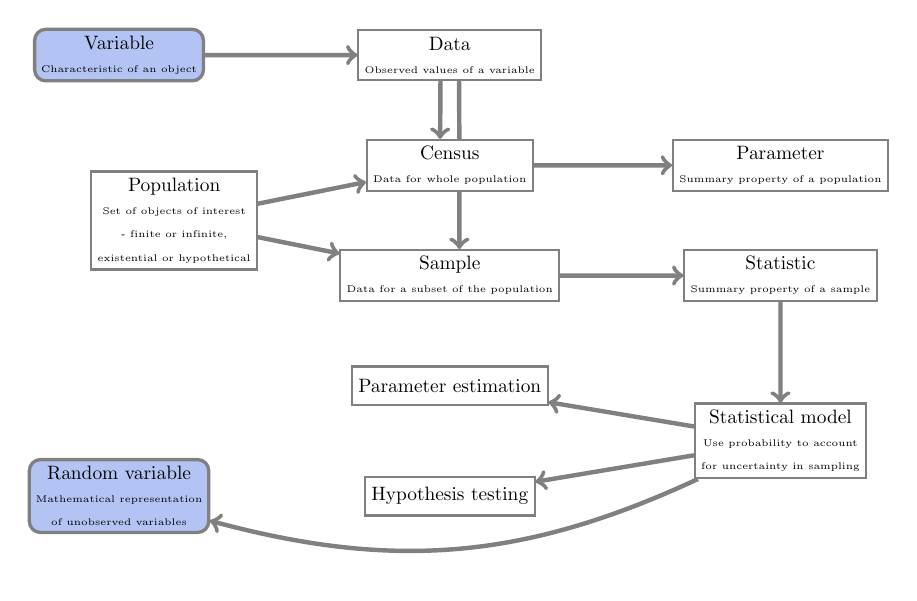
\begin{tikzpicture}[scale=.7,transform shape,thick,
			main node/.style={
				rectangle, draw=black!50, very thick,
				fill=RoyalBlue!40,align=center,
				text=black, rounded corners, minimum height=2em},
			second node/.style={
				rectangle, draw=black!50, thick,
				fill=white, text=black, align=center,
				minimum height=2em,minimum width=25pt}
			]
			\node[main node,minimum width=25pt] (1) at (0,10)
			{Variable\\{\tiny Characteristic of an object}};
			\node[second node] (2) at (6,10)
			{Data\\{\tiny Observed values of a variable}};
			\node[second node] (3) at (1,7)
			{Population\\{\tiny Set of objects of interest}\\{\tiny - finite or infinite,}\\{\tiny existential or hypothetical}};
			\node[second node] (4) at (6,8)
			{Census\\{\tiny Data for whole population}};
			\node[second node] (5) at (6,6)
			{Sample\\{\tiny Data for a subset of the population}};
			\node[second node] (6) at (12,8)
			{Parameter\\{\tiny Summary property of a population}};
			\node[second node] (7) at (12,6)
			{Statistic\\{\tiny Summary property of a sample}};
			\node[second node] (8) at (12,3)
			{Statistical model\\{\tiny Use probability to account}\\{\tiny for uncertainty in sampling}};
			\node[second node] (9) at (6,4)
			{Parameter estimation};
			\node[second node] (10) at (6,2)
			{Hypothesis testing};
			\node[main node] (11) at (0,2)
			{Random variable\\{\tiny Mathematical representation}\\{\tiny of unobserved variables}};
			
			\path[every node/.style={font=\sffamily\small}]
			(1) edge[->,ultra thick, black!50] (2)
			(2.250) edge[->,ultra thick, black!50] (4.110)
			(2.290) edge[ultra thick, black!50] (4.70)
			(4.290) edge[->,ultra thick, black!50] (5.70)
			(3) edge[->,ultra thick, black!50] (4)
			(3) edge[->,ultra thick, black!50] (5)
			(4) edge[->,ultra thick, black!50] (6)
			(5) edge[->,ultra thick, black!50] (7)
			(7) edge[->,ultra thick, black!50] (8)
			(8) edge[->,ultra thick, black!50] (9)
			(8) edge[->,ultra thick, black!50] (10)
			(8) edge[->,ultra thick, black!50,bend left=20] (11);
		\end{tikzpicture}
	\end{frame}
	
	% ------------------------------------------------------------
	\begin{frame}
		\frametitle{Data types}
		\begin{itemize}
			\item {\bf Qualitative:} categories/groups
			\begin{itemize}
				\item {\bf Categorical/nominal:} mutually exclusive, unordered. \par
				Examples: sex, subject of study, hometown.
				\item {\bf Ordinal:} mutually exclusive, order matters. \par
				Examples: education level (BSc, MSc, PhD), military rank.
			\end{itemize}
			\item {\bf Quantitative:} measured numerical values \par
			- naturally ordered.
			\begin{itemize}
				\item {\bf Interval:} differences between values are meaningful, but zero is arbitrary. \par
				Examples: temperature (Celsius/Fahrenheit), IQ score, calendar time.
				\item {\bf Ratio:} zero means ``none''. \par
				Examples: temperature (Kelvin), age, length.
			\end{itemize}
		\end{itemize}
	\end{frame}
	
	% ------------------------------------------------------------
	\begin{frame}
		\frametitle{Data types}
		\begin{itemize}
			\item {\bf Quantitative (continued):}
			\begin{itemize}
				\item {\bf Discrete:} distinct, countable values. \par
				Examples: number of children, shoe size, age (in years), outcome of rolling a die.
				\item {\bf Continuous:} can take any value in a given range (uncountably many). \par
				Examples: temperature, foot length, luminosity, electrical power.
			\end{itemize}
		\end{itemize}
	\end{frame}
	
	% ------------------------------------------------------------
	\begin{frame}
		\frametitle{Data types}
		{\bf\underline{Exercise}} \par
		Classify the following variables using the terms: \par
		qualitative (categorical/ordinal), quantitative (interval/ratio, discrete/continuous).
		\begin{itemize}
			\item T–shirt size (XS, S, M, L, XL)
			\item Moderated exam score in MATH163 (0–100 scale)
			\item Preferred study method (Group, Solo, Procrastination)
			\item Satisfaction with campus facilities \par
			(Very Dissatisfied, Dissatisfied, Neutral, Satisfied, Very Satisfied)
			\item Number of classes taken this semester (USA)
			\item Major/field of study
			\item Height of students (in centimetres)
			\item Number of days absent from lectures in a month
		\end{itemize}
	\end{frame}
	
	% ------------------------------------------------------------
	\begin{frame}
		\frametitle{Summary statistics: intuition}
		\begin{itemize}
			\item {\bf Mean:} the ``centre of mass'' of the data
			{\color{black!40}
				\item {\bf Mode:} the most common value
				\item {\bf Median:} the midpoint of the ordered data
				\item {\bf Percentiles} (typically $0,5,25,50,75,95,100$)
			}
			{\color{black!40}
				\item {\bf Range:} difference between largest and smallest value
				\item {\bf Interquartile range (IQR):} 75th–25th percentile
				\item {\bf Mean absolute deviation:} mean distance from the mean
			}
			\item {\bf Variance:} mean squared distance from the mean
			\item {\bf Standard deviation:} square root of variance
			{\color{black!40}
				\item {\bf Skewness:} measure of symmetry
				\item {\bf Kurtosis:} measure of ``spikiness''
			}
		\end{itemize}
	\end{frame}
	
	% ------------------------------------------------------------
	\begin{frame}
		\frametitle{Summary statistics: definitions}
		Let $x_i,\ i=1,2,\dots,n$ be $n$ measurements of a numeric variable. \par
		This is our {\bf data}. \par
		{\bf\underline{Mean}:}
		\[
		\mu := \frac{1}{n}\sum_{i=1}^n x_i
		\]
		{\bf\underline{Variance}:}
		\[
		\sigma^2 := \frac{1}{n}\sum_{i=1}^n (x_i-\mu)^2
		\]
		Questions:
		\begin{itemize}
			\item What is the difference between standard deviation $\sigma$ and mean absolute deviation $MAD$?
			\[
			\sigma := \sqrt{\frac{1}{n}\sum_{i=1}^n (x_i-\mu)^2},\qquad
			MAD := \frac{1}{n}\sum_{i=1}^n |x_i-\mu|
			\]
			\item What are the advantages/disadvantages of each?
		\end{itemize}
	\end{frame}
	
	% ------------------------------------------------------------
	\begin{frame}
		\frametitle{Box plots}
		Box plots are used to display percentiles:
		\begin{itemize}
			\item The ``box'' displays the 25th, 50th and 75th percentiles
			\item Outliers are typically $>1.5\times IQR$ outside the box
			\item ``Whiskers'' show the range of the data excluding outliers
			\item ``Left''/``negative'' skew: a tail to the left (mean $<$
			median)
			\item ``Right''/``positive'' skew: a tail to the right (mean $>$
			median)
		\end{itemize}
		\begin{center}
			\fbox{\includegraphics[width=.5\textwidth]{boxplots.png}}
		\end{center}
		{\small\color{NavyBlue} Box plots typically do not show the mean, so skewness is only clear if the box and whisker are larger on the same side of the median.}
	\end{frame}
	
	% ------------------------------------------------------------
	\begin{frame}
		\frametitle{Random variables}
		A random variable describes the outcome of a measurement \par
		{\bf before} the measurement has happened. \par
		{\bf Example:} rolling a die. \par
		10 die rolls gave the numbers $6,6,2,4,6,6,2,6,4,2$ — this is data. \par
		Before rolling, the random variable $X$ denotes the outcome:
		\[
		p_X(x) =
		\begin{cases}
			\frac{1}{6}, & x=1,2,3,4,5,6,\\[4pt]
			0, & \text{otherwise.}
		\end{cases}
		\]
		\begin{center}
			\fbox{\includegraphics[width=.2\textwidth]{dice.png}}
		\end{center}
	\end{frame}
	
	% ------------------------------------------------------------
	\begin{frame}
		\frametitle{Random variables}
		{\bf\underline{Definition}} \par
		A random variable is a mathematical formalisation of a quantity or object which depends on random events. \par
		Its value is unknown, but a probability mass function (PMF) or probability density function (PDF) is used to associate probabilities to different outcomes.
	\end{frame}
	
	% ------------------------------------------------------------
	\begin{frame}
		\frametitle{Random variables: discrete or continuous}
		\begin{columns}
			\column{0.5\textwidth}
			Discrete case:
			\begin{center}
				\vspace{5pt}
				\fbox{\includegraphics[width=\textwidth]{pmf.png}}
			\end{center}
			Probability mass function (PMF)
			\begin{itemize}
				\item PMF defines $P(X=x)$
				\item Values are probabilities
				\item ``Ready–integrated'' — sum over values for probabilities
			\end{itemize}
			\column{0.5\textwidth}
			Continuous case:
			\begin{center}
				\vspace{5pt}
				\fbox{\includegraphics[width=\textwidth]{pdf.png}}
			\end{center}
			Probability density function (PDF)
			\begin{itemize}
				\item $P(X=x)=0$ for all $x$
				\item $f_X(x)$ has dimension $1/(\text{unit of }x)$
				\item PDF describes how probability changes with $x$
				\item Integrate for probabilities
			\end{itemize}
		\end{columns}
	\end{frame}
	
	% ------------------------------------------------------------
	\begin{frame}
		\frametitle{Cumulative density: continuous case}
		\begin{columns}
			\column{0.5\textwidth}
			\begin{center}
				\vspace{5pt}
				\fbox{\includegraphics[width=\textwidth]{pdf.png}}
			\end{center}
			\column{0.5\textwidth}
			\begin{center}
				\vspace{5pt}
				\fbox{\includegraphics[width=\textwidth]{cdfcont.png}}
			\end{center}
		\end{columns}
		Cumulative distribution function (CDF): \par
		\[
		F_X(x) := P(X \le x).
		\]
		In the continuous case, this is the integral of the PDF:
		\[
		F_X(x) = \int_{-\infty}^{x} f_X(t)\,dt.
		\]
	\end{frame}
	
	% ------------------------------------------------------------
	\begin{frame}
		\frametitle{Cumulative density: discrete case}
		\begin{columns}
			\column{0.5\textwidth}
			\begin{center}
				\vspace{5pt}
				\fbox{\includegraphics[width=\textwidth]{pmf.png}}
			\end{center}
			\column{0.5\textwidth}
			\begin{center}
				\vspace{5pt}
				\fbox{\includegraphics[width=\textwidth]{cdfdisc.png}}
			\end{center}
		\end{columns}
		Cumulative distribution function (CDF): \par
		\[
		F_X(x) := P(X \le x).
		\]
		The discrete case is still defined as a function of a continuous variable $x$, \par
		but the function $F_X(x)$ has jumps — it is not continuous.
	\end{frame}
	
	% ------------------------------------------------------------
	\begin{frame}
		\frametitle{Notation}
		For a random variable $X$ and value $x$, we define:
		\begin{itemize}
			\item $p_X(x) = P(X=x)$ — PMF (discrete)
			\item $F_X(x) = P(X\le x)$ — CDF
			\item $f_X(x)$ — PDF: $\displaystyle\int_a^b f_X(x)\,dx = P(a\le X\le b)$
			\item $F_X(x) := P(X\le x)$ — CDF
			\item $E[X]$ — mean or expected value of $X$
			\item $\sigma^2(X)=\mathrm{Var}(X)$ — variance of $X$
		\end{itemize}
	\end{frame}
	
	\begin{frame}
		\frametitle{Warning}
		Sometimes continuous random variables are described by ``nice'' functions, but only on specific intervals. \par
		Example:
		\begin{eqnarray*}
			f_X(x) = \left\{\begin{array}{ll}
				\dfrac 1c(x^3-7x^2+15x-7), & x\in(1,4)\\[3pt]
				0, & \text{otherwise}
			\end{array}\right.
		\end{eqnarray*}
		\begin{columns}
			\column{0.5\textwidth}
			\centering
			\fbox{\includegraphics[width=\textwidth]{contEgW3a.png}}\\[3pt]
			PDF
			\column{0.5\textwidth}
			\centering
			\fbox{\includegraphics[width=\textwidth]{contEgW3b.png}}\\[3pt]
			CDF
		\end{columns}
	\end{frame}
	
	\begin{frame}
		\frametitle{Warning}
		\color{gray}
		Sometimes continuous random variables are described by ``nice'' functions, but only on specific intervals. \par
		Example:
		\begin{eqnarray*}
			f_X(x) = \left\{\begin{array}{ll}
				\dfrac 1c(x^3-7x^2+15x-7), & x\in(1,4)\\[3pt]
				0, & \text{otherwise}
			\end{array}\right.
		\end{eqnarray*}
		\color{black}
		Important observation:
		\begin{eqnarray*}
			\int_{-\infty}^{\infty} f_X(x)\,dx
			&=&\frac 1c\int_1^4 (x^3-7x^2+15x-7)\,dx = 1\\
			&\neq&\frac 1c\int_{-\infty}^{\infty} (x^3-7x^2+15x-7)\,dx
		\end{eqnarray*}
		- be careful with the limits on the integral! \par
		{\bf We will not always use $X$ for a discrete and $Y$ for a continuous random variable — beware of context!}
	\end{frame}
	
	\begin{frame}
		\frametitle{Histograms vs bar charts}
		{\bf\underline{Histograms}} \par
		Used for {\bf quantitative} (usually continuous) data
		\begin{itemize}
			\item Data are grouped into {\bf bins} (intervals on the $x$-axis)
			\item The {\bf area} of each bar is proportional to the frequency (or relative frequency) in that bin
			\item If all bins have equal width, then the {\bf height} is proportional to frequency
			\item Bars {\bf touch}: the order of bins and continuity on the $x$-axis matter
		\end{itemize}
		{\bf\underline{Bar charts}} \par
		Used for {\bf categorical} (or discrete) data
		\begin{itemize}
			\item One bar per category (e.g. ``red", ``blue", ``green")
			\item The height of each bar shows the frequency (or proportion) of that category
			\item Bar {\bf width} is arbitrary – only the height encodes information
			\item Bars are usually {\bf separated by gaps}; the order of categories is often arbitrary
		\end{itemize}
	\end{frame}
	
	\begin{frame}
		\frametitle{Histograms vs bar charts}
		\begin{columns}
			\column{0.5\textwidth}
			\centering
			\fbox{\includegraphics[width=\textwidth]{histogram.png}}\\[3pt]
			Histogram/PMF
			\column{0.5\textwidth}
			\centering
			\fbox{\includegraphics[width=\textwidth]{barChart.png}}\\[3pt]
			Bar chart/points
		\end{columns}
		\begin{itemize}
			\item Histograms typically approximate PDFs
			\item Bar charts typically depict PMFs
		\end{itemize}
	\end{frame}
	
	%\begin{frame}
	%  \frametitle{Random variables vs. functions}
	%  Functions give a single output for each input:
	%  \begin{eqnarray*}
		%    f:U&\rightarrow&V\\
		%    u\in U &\mapsto& v\in V
		%  \end{eqnarray*}
	%  Random variables have no input: they are specified by assigning probabilities to events. \par
	%  PMFs, PDFs and CDFs are functions of the \emph{outcome} of a random variable. \par
	%\end{frame}
	
	% ------------------------------------------------------------
	\begin{frame}
		\frametitle{Random variables: mean}
		For a data set $\{X_1,X_2,\dots,X_n\}$, the sample mean is
		\[
		\mu := \frac{1}{n}\sum_{i=1}^n X_i.
		\]
		{\small\color{NavyBlue} We are summing over all data points but some of them may be repeated.} \par
		If the number $x_j$ occurs $k_j$ times then
		\[
		\mu = \frac{1}{n}\sum_j k_j x_j = \sum_j \frac{k_j}{n}x_j.
		\]
		{\small\color{NavyBlue} Now we are summing over the possible values of $X$, not the data points themselves.} \par
		Note that $\frac{k_j}{n}$ is the proportion of data points that take the value $x_j$. \par
		{\bf\underline{Definition}} (discrete case). If $X$ has PMF $p_X(x)$:
		\[
		E[X] := \sum_j x_j\,p_X(x_j).
		\]
		%By analogy, 
		For a continuous random variable $Y$ with PDF $f_Y(y)$:
		\[
		E[Y] := \int_{-\infty}^{\infty} y\,f_Y(y)\,dy.
		\]
	\end{frame}
	
	% ------------------------------------------------------------
	\begin{frame}
		\frametitle{Random variables: variance}
		Question: Why do we not typically use
		\[
		MAD := \frac{1}{n}\sum_i |x_i-\mu|?
		\]
		Answer: Mean {\bf squared} distance arises naturally in many contexts. \par
		Motivation:
		\begin{align*}
			\frac{1}{n}\sum_i (x_i-\mu)^2
			&= \frac{1}{n}\sum_i (x_i^2 - 2\mu x_i + \mu^2) \\
			&= \left[\frac{1}{n}\sum_i x_i^2\right]
			- \left[\frac{2\mu}{n}\sum_i x_i\right]
			+ \left[\frac{\mu^2}{n}\sum_i 1\right] \\
			&= \left[\frac{1}{n}\sum_i x_i^2\right] - 2\mu^2 + \mu^2 \\
			&= \left[\frac{1}{n}\sum_i x_i^2\right] - \mu^2.
		\end{align*}
		{\small\color{NavyBlue} ``The mean of the square minus the square of the mean.''}
	\end{frame}
	
	% ------------------------------------------------------------
	\begin{frame}
		\frametitle{Random variables: variance}
		{\bf\underline{Definition}} \par
		The variance of a discrete random variable $X$ with PMF $p_X(x)$ is
		\begin{align*}
			\mathrm{Var}(X)
			&= \sum_j (x_j-\mu)^2\,p_X(x_j) \\
			&= E[X^2] - E[X]^2.
		\end{align*}
		By analogy, for a continuous random variable $Y$ with PDF $f_Y(y)$:
		\begin{align*}
			\mathrm{Var}(Y)
			&= \int_{-\infty}^{\infty} (y-\mu)^2 f_Y(y)\,dy \\
			&= E[Y^2] - E[Y]^2.
		\end{align*}
		Question: what about the mean of the cube, power 4, etc? (Higher moments.)
	\end{frame}
	
	% ------------------------------------------------------------
	\begin{frame}
		\frametitle{Random variables: mode and median}
		Let $X$ be a random variable with domain (sample space) $\Omega$. \par
		{\bf\underline{Median}}
		\[
		\mathrm{med}(X) := F_X^{-1}\!\left(\frac{1}{2}\right)
		\]
		{\small\color{NavyBlue}
			This is the inverse of the CDF at $1/2$. \par
			Note: this can be a set rather than a single value (cf.\ Bernoulli distribution).} \par
		{\bf\underline{Mode}}
		\begin{align*}
			\mathrm{mode}(X)
			&= \{\,x\in\Omega \mid p_X(x) = \max_{\Omega} p_X(x)\,\}
			&& \text{(discrete)}\\
			\mathrm{mode}(X)
			&= \{\,x\in\Omega \mid f_X(x) = \max_{\Omega} f_X(x)\,\}
			&& \text{(continuous)}
		\end{align*}
		{\small\color{NavyBlue} The set of values of $X$ at which the PMF/PDF takes its maximum value.}
	\end{frame}
	
	% ------------------------------------------------------------
	\begin{frame}
		\frametitle{Transition to R}
		The practical materials will provide all necessary information to set up an R session — {\bf follow them step by step}. \par
		Here are some key commands for working with data:
		{\footnotesize
			\begin{itemize}
				\item Frequency: \texttt{table(df\$variable)}
				\item Median: \texttt{median(x)}
				\item Order data values: \texttt{sort(x)}
				\item Mean: \texttt{mean(x)}
				\item IQR: \texttt{IQR(x)}
				\item Summary: \texttt{summary(x)}
				\item Boxplot: \texttt{boxplot(x)}
				\item Plots: \texttt{plot(x)}, \texttt{barplot(x)}, \texttt{hist(x)}
				\item Variance: \texttt{var(x)}
				\item Standard deviation: \texttt{sd(x)}
			\end{itemize}
		}
		{\small
			Note: \texttt{df} is a data frame, and \texttt{\$} indexes a column by its name. \par
			In lectures: compare the value of \texttt{var(x)} with the manually computed value. \par
			\color{NavyBlue} This motivates the concept of ``sample variance'' studied in week 7.}
	\end{frame}
	
	\begin{frame}
		\frametitle{Example 1A: the uniform distribution $U(a,b)$}
		Let $X$ be a continuous random variable with {\bf uniform} distribution on the interval $(a,b)$, where $a<b$. \par
		This means that all values in $(a,b)$ are equally likely. Suppose the PDF of $X$ is
		\[
		f_X(x) =
		\begin{cases}
			k, & a < x < b,\\
			0, & \text{otherwise},
		\end{cases}
		\]
		for some constant $k>0$.
		
		{\bf\underline{Questions}}
		\begin{itemize}
			\item[(a)] Find the constant $k$. 
			\item[(b)] Hence compute the mean $E[X]$ and the variance $\mathrm{Var}(X)$. 
			\item[(c)] Find the median $m$ of $X$. 
		\end{itemize}
		Hint: draw a picture. \par
		{\small\color{NavyBlue} Drawing a picture is an almost guaranteed way of getting your head around ANY question.}
	\end{frame}
	
	\begin{frame}
		\frametitle{Example 1A: the uniform distribution $U(a,b)$ (answer)}
		%For $X \sim U(a,b)$ with PDF
		\[
		X \sim U(a,b):\quad f_X(x) =
		\begin{cases}
			k, & a < x < b,\\
			0, & \text{otherwise},
		\end{cases}
		\]
		%we have:
		
		\vspace{4pt}
		{\bf (a) Normalising constant}
		\[
		\int_{-\infty}^{\infty} f_X(x)\,dx
		= \int_a^b k\,dx = k(b-a) = 1
		\;\Rightarrow\; k = \frac{1}{b-a}.
		\]
		
		{\bf (b) Mean and variance}
		\[
		E[X] = \int_a^b x \frac{1}{b-a}\,dx 
		= \frac{1}{b-a}\left[\frac{x^2}{2}\right]_a^b
		= \frac{a+b}{2},
		\]
		\[
		E[X^2] = \int_a^b x^2 \frac{1}{b-a}\,dx
		= \frac{1}{b-a}\left[\frac{x^3}{3}\right]_a^b
		= \frac{a^2+ab+b^2}{3},
		\]
		\[
		\mathrm{Var}(X) = E[X^2] - (E[X])^2 
		= \frac{(b-a)^2}{12}.
		\]
		
		{\bf (c) Median}
		The median $m$ satisfies
		\[
		P(X \le m) = \int_a^m \frac{1}{b-a}\,dx = \frac{m-a}{b-a} = \frac{1}{2}
		\;\Rightarrow\; m = \frac{a+b}{2}.
		\]
	\end{frame}
	
	
	\begin{frame}
		\frametitle{Example 1B: PDF on a finite interval}
		
		Let $X$ be a continuous random variable with PDF
		\[
		f_X(x) = \begin{cases}
			k\,x^2(2-x), & 0 < x < 2,\\[4pt]
			0, & \text{otherwise.}
		\end{cases}
		\]
		
		\begin{itemize}
			\item[(a)] Find the value of $k$ that makes $f_X$ a valid PDF.
			\item[(b)] Hence derive the CDF $F_X(x)$.
			\item[(c)] Compute the mean $E[X]$.
			\item[(d)] Find the median $m$, i.e.\ solve $F_X(m)=\tfrac12$. \par
			{\small\color{NavyBlue} (You may leave $m$ as the solution of an equation, or give a numerical approximation.)}
		\end{itemize}
		
		%\begin{center}
		%  \fbox{\includegraphics[width=.2\textwidth]{countdown.jpg}}
		%\end{center}
	\end{frame}
	
	\begin{frame}
		\frametitle{Example 1C: working from a CDF}
		
		A continuous random variable $X$ has CDF
		\[
		F_X(x) =
		\begin{cases}
			0, & x \le 0,\\[4pt]
			1 - \dfrac{k}{(x+1)^3}, & x > 0,
		\end{cases}
		\]
		for some constant $k>0$.
		
		\begin{itemize}
			\item[(a)] Find $k$ so that $F_X$ is a valid CDF  
			%{\small\color{NavyBlue} (i.e.\ $F_X$ is continuous at $0$ and $\lim_{x\to\infty}F_X(x)=1$).}
			\item[(b)] Differentiate $F_X$ to obtain the PDF $f_X(x)$.
			\item[(c)] Compute the mean $E[X]$.
			\item[(d)] Compute the variance $\mathrm{Var}(X)$.
		\end{itemize}
		
		\begin{center}
			\fbox{\includegraphics[width=.2\textwidth]{countdown.jpg}}
		\end{center}
	\end{frame}
	
	\begin{frame}
		\frametitle{Example 1D: discrete heavy-tailed distribution}
		
		Let $X$ take values $k=1,2,3,\dots$ with PMF
		\[
		p_X(k) = \frac{C}{k^2}, \qquad k = 1,2,\dots
		\]
		where $C$ is a normalising constant.
		
		\begin{itemize}
			\item[(a)] Find the approximate value of $C$. \par
			%Show that $\displaystyle \sum_{k=1}^{\infty}\frac{1}{k^2} < \infty$ and hence find $C$. \par
			%{\small\color{NavyBlue} (You may use the fact $\displaystyle \sum_{k=1}^{\infty}\frac{1}{k^2} = \frac{\pi^2}{6}$.)}
			{\small\color{NavyBlue} (You may need to look up a standard result: $\displaystyle \sum_{k=1}^{\infty}\frac{1}{k^2} = ?$)}
			\item[(b)] Find the mean and variance of $X$.
			\item[(c)] What can you say about discrete random variables of the form:
			\[
			p_X(k) = \frac{C}{k^{\alpha}}, \qquad k = 1,2,\dots .
			\]
			%Show that the variance $\mathrm{Var}(X)$ is also infinite.
			%{\small\color{NavyBlue} (Hint: consider $E[X^2]$.)}
		\end{itemize}
		
		\begin{center}
			\fbox{\includegraphics[width=.2\textwidth]{countdown.jpg}}
		\end{center}
	\end{frame}
	
	
	% ------------------------------------------------------------

% ============================================================
% Week 2
% ============================================================

\section{Week 2: probability for statistics}

\begin{frame}
	\frametitle{Probability: example 2A}
	\begin{columns}[T]
		\column{0.6\textwidth}
		{\footnotesize
			In the 1980s, the incidence of cervical cancer in the UK was estimated at about 15 per 100,000 women annually.  
			With approximately 15 million women eligible for screening, around 2,250 new cases of cervical cancer were diagnosed each year. \par
			\vspace{5pt}
			Roughly 70–80\% of eligible women participated in cervical screening programmes. This means about 10.5–12 million women underwent smear tests annually. Of these, a relatively small percentage had pre-cancerous changes (cervical intraepithelial neoplasia or CIN) or undiagnosed cancer. \par
			\vspace{5pt}
			With a false positive rate of about 20–30\%, 2.1–3.6 million women may have received abnormal results despite being healthy.
			These women would have undergone further testing (e.g.\ colposcopy) to confirm or rule out actual abnormalities. \par
			\vspace{5pt}
			The false negative rate was around 5–15\%, meaning that of the estimated 2,250 women with cervical cancer, approximately 113–338 women were missed annually during screening. These women would likely only be diagnosed when their cancer advanced, reducing treatment options and worsening prognosis. \par
		}
		\column{0.4\textwidth}
		\centering
		\includegraphics[width=\textwidth]{cervical.jpg}
	\end{columns}
\end{frame}

\begin{frame}
	\frametitle{Probability: example 2A}
	\begin{columns}[T]
		\column{0.6\textwidth}
		{\bf\underline{Summary}} \par
		\begin{itemize}
			\item $0.00015$ of the female population is estimated to develop cancer per year
			\item $10.5$–$12$ million women underwent annual screening (assume $12$ million)
			\item False positive rate $\approx 20$–$30\%$ (assume $20\%$)
			\item False negative rate $\approx 5$–$15\%$ (assume $5\%$)
		\end{itemize}
		\vspace{5pt}
		{\bf\underline{Question}} \par
		A woman tests positive. What is the probability she has cervical cancer/pre-cancerous cells?
		\column{0.4\textwidth}
		\centering
		\includegraphics[width=\textwidth]{cervical.jpg}
	\end{columns}
\end{frame}

\begin{frame}
	\frametitle{What is probability?}
	{\bf\underline{Intuition}} \par
	Probability is a measure of uncertainty about anything that has not yet been observed. \par
	{\small\color{NavyBlue} - random variables represent ``unobserved data", so they are described in terms of probability.} \par
	In A-level maths:
	\begin{itemize}
		\item $P(A)$ denotes the probability of an event occurring
		\item $A\cup B$ means ``$A$ or $B$"
		\item $A\cap B$ means ``$A$ and $B$"
		\item $\overline A,\ A^C$ or $A'$ means ``not $A$"
		\item $A\vert B$ means ``$A$ given $B$"
	\end{itemize}
	Is this notation familiar from other modules?
\end{frame}

\begin{frame}
	\frametitle{Outcomes and events}
	{\bf\underline{Definitions}} \par
	An {\bf outcome} is a single value that a random variable can take. \par
	An {\bf event} is a set of outcomes. \par
	The {\bf outcome space} or {\bf event space} is the set of all possible outcomes of a random variable (and therefore contains all possible events). \par
	{\bf The notation $P(A)$ is shorthand for $P(X\in A)$.} \par
	Examples:
	\begin{itemize}
		\item Coin toss: $\Omega=\{H,T\}$; possible events are $\{H\}$, $\{T\}$ and $\{H,T\}$
		\item Dice roll: $\Omega=\{1,2,3,4,5,6\}$; the event of rolling an even number is the set $\{2,4,6\}$
		\item Pick a card: $\Omega=\{\text{all $52$ cards}\}$; the event of drawing a Jack is $\{J\clubsuit,J\spadesuit,J\heartsuit,J\diamondsuit\}$
		\item Height of students (in metres): $\Omega=(0,\infty)$; the event that a student exceeds $6$ft is $(182.88,\infty)$
	\end{itemize}
	Convention: for finite random variables, we typically exclude from $\Omega$ outcomes with probability $0$.
\end{frame}

%\begin{frame}
%  \frametitle{Set theory: recap}
%  \includegraphics[width=\textwidth]{setVenn.png}
%\end{frame}

\begin{frame}
	\frametitle{Set theory: recap}
	\begin{center}
		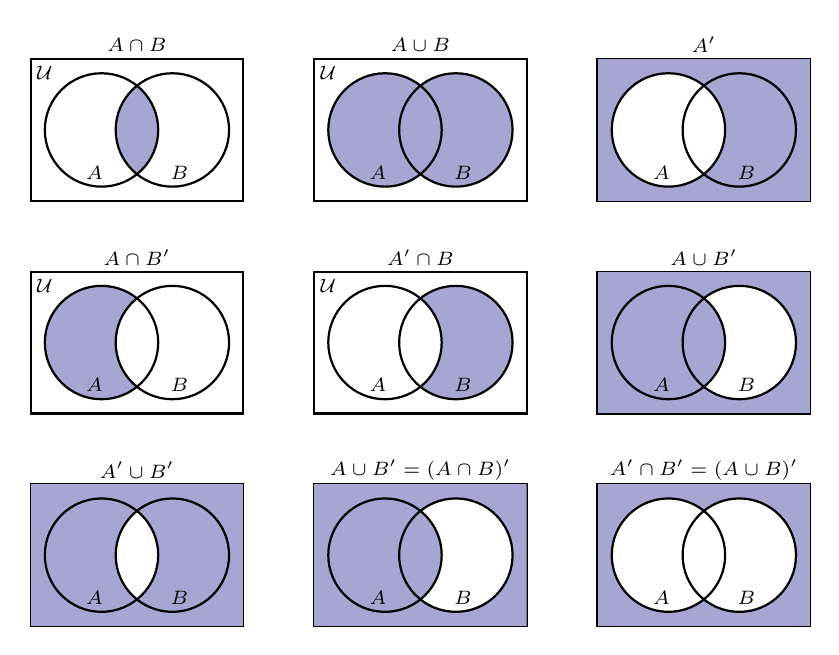
\begin{tikzpicture}[scale=0.9]
			\colorlet{vennfill}{NavyBlue!35}
			\colorlet{vennedge}{black}
			
			% ---------- Row 1: A∩B, A∪B, A' ----------
			% A ∩ B
			\begin{scope}[shift={(0,5)}]
				\draw[thick] (0,0) rectangle (3,2);
				\node[font=\scriptsize] at (0.2,1.8) {$\mathcal{U}$};
				
				% shaded: intersection
				\begin{scope}
					\clip (1,1) circle (0.8);
					\fill[vennfill] (2,1) circle (0.8);
				\end{scope}
				
				\draw[vennedge,thick] (1,1) circle (0.8);
				\draw[vennedge,thick] (2,1) circle (0.8);
				\node[font=\scriptsize] at (0.9,0.4) {$A$};
				\node[font=\scriptsize] at (2.1,0.4) {$B$};
				\node[font=\scriptsize] at (1.5,2.2) {$A\cap B$};
			\end{scope}
			
			% A ∪ B
			\begin{scope}[shift={(4,5)}]
				\draw[thick] (0,0) rectangle (3,2);
				\node[font=\scriptsize] at (0.2,1.8) {$\mathcal{U}$};
				
				% shaded: union
				\fill[vennfill] (1,1) circle (0.8);
				\fill[vennfill] (2,1) circle (0.8);
				
				\draw[vennedge,thick] (1,1) circle (0.8);
				\draw[vennedge,thick] (2,1) circle (0.8);
				\node[font=\scriptsize] at (0.9,0.4) {$A$};
				\node[font=\scriptsize] at (2.1,0.4) {$B$};
				\node[font=\scriptsize] at (1.5,2.2) {$A\cup B$};
			\end{scope}
			
			% A'
			\begin{scope}[shift={(8,5)}]
				\draw[thick] (0,0) rectangle (3,2);
				\node[font=\scriptsize] at (0.2,1.8) {$\mathcal{U}$};
				
				% shaded: complement of A
				\begin{scope}
					\clip (0,0) rectangle (3,2);
					\fill[vennfill] (0,0) rectangle (3,2);
					\fill[white] (1,1) circle (0.8);
				\end{scope}
				
				\draw[vennedge,thick] (1,1) circle (0.8);
				\draw[vennedge,thick] (2,1) circle (0.8);
				\node[font=\scriptsize] at (0.9,0.4) {$A$};
				\node[font=\scriptsize] at (2.1,0.4) {$B$};
				\node[font=\scriptsize] at (1.5,2.2) {$A'$};
			\end{scope}
			
			% ---------- Row 2: A∩B', A'∩B, A∪B' ----------
			% A ∩ B'
			\begin{scope}[shift={(0,2)}]
				\draw[thick] (0,0) rectangle (3,2);
				\node[font=\scriptsize] at (0.2,1.8) {$\mathcal{U}$};
				
				% shaded: A but not B
				\begin{scope}
					\clip (1,1) circle (0.8);
					\fill[vennfill] (0,0) rectangle (3,2);
					\fill[white] (2,1) circle (0.8);
				\end{scope}
				
				\draw[vennedge,thick] (1,1) circle (0.8);
				\draw[vennedge,thick] (2,1) circle (0.8);
				\node[font=\scriptsize] at (0.9,0.4) {$A$};
				\node[font=\scriptsize] at (2.1,0.4) {$B$};
				\node[font=\scriptsize] at (1.5,2.2) {$A\cap B'$};
			\end{scope}
			
			% A' ∩ B
			\begin{scope}[shift={(4,2)}]
				\draw[thick] (0,0) rectangle (3,2);
				\node[font=\scriptsize] at (0.2,1.8) {$\mathcal{U}$};
				
				% shaded: B but not A
				\begin{scope}
					\clip (2,1) circle (0.8);
					\fill[vennfill] (0,0) rectangle (3,2);
					\fill[white] (1,1) circle (0.8);
				\end{scope}
				
				\draw[vennedge,thick] (1,1) circle (0.8);
				\draw[vennedge,thick] (2,1) circle (0.8);
				\node[font=\scriptsize] at (0.9,0.4) {$A$};
				\node[font=\scriptsize] at (2.1,0.4) {$B$};
				\node[font=\scriptsize] at (1.5,2.2) {$A'\cap B$};
			\end{scope}
			
			% A ∪ B'
			\begin{scope}[shift={(8,2)}]
				\draw[thick] (0,0) rectangle (3,2);
				\node[font=\scriptsize] at (0.2,1.8) {$\mathcal{U}$};
				
				% shaded: A ∪ B' = (outside B) plus A
				\begin{scope}
					\clip (0,0) rectangle (3,2);
					\fill[vennfill] (0,0) rectangle (3,2); % everything
					\fill[white] (2,1) circle (0.8);       % remove B
					\fill[vennfill] (1,1) circle (0.8);    % add A back
				\end{scope}
				
				\draw[vennedge,thick] (1,1) circle (0.8);
				\draw[vennedge,thick] (2,1) circle (0.8);
				\node[font=\scriptsize] at (0.9,0.4) {$A$};
				\node[font=\scriptsize] at (2.1,0.4) {$B$};
				\node[font=\scriptsize] at (1.5,2.2) {$A\cup B'$};
			\end{scope}
			
			% ---------- Row 3: A'∪B', A∪B'=(A∩B)', A'∩B'=(A∪B)' ----------
			% A' ∪ B'
			\begin{scope}[shift={(0,-1)}]
				\draw[thick] (0,0) rectangle (3,2);
				\node[font=\scriptsize] at (0.2,1.8) {$\mathcal{U}$};
				
				% shaded: complement of A∩B
				\begin{scope}
					\clip (0,0) rectangle (3,2);
					\fill[vennfill] (0,0) rectangle (3,2); % everything
					\begin{scope}
						\clip (1,1) circle (0.8);
						\fill[white] (2,1) circle (0.8);    % remove intersection
					\end{scope}
				\end{scope}
				
				\draw[vennedge,thick] (1,1) circle (0.8);
				\draw[vennedge,thick] (2,1) circle (0.8);
				\node[font=\scriptsize] at (0.9,0.4) {$A$};
				\node[font=\scriptsize] at (2.1,0.4) {$B$};
				\node[font=\scriptsize] at (1.5,2.2) {$A'\cup B'$};
			\end{scope}
			
			% A ∪ B' = (A ∩ B)'
			\begin{scope}[shift={(4,-1)}]
				\draw[thick] (0,0) rectangle (3,2);
				\node[font=\scriptsize] at (0.2,1.8) {$\mathcal{U}$};
				
				% same shading as A∪B'
				\begin{scope}
					\clip (0,0) rectangle (3,2);
					\fill[vennfill] (0,0) rectangle (3,2);
					\fill[white] (2,1) circle (0.8);
					\fill[vennfill] (1,1) circle (0.8);
				\end{scope}
				
				\draw[vennedge,thick] (1,1) circle (0.8);
				\draw[vennedge,thick] (2,1) circle (0.8);
				\node[font=\scriptsize] at (0.9,0.4) {$A$};
				\node[font=\scriptsize] at (2.1,0.4) {$B$};
				\node[font=\scriptsize] at (1.5,2.2) {$A\cup B' = (A\cap B)'$};
			\end{scope}
			
			% A' ∩ B' = (A ∪ B)'
			\begin{scope}[shift={(8,-1)}]
				\draw[thick] (0,0) rectangle (3,2);
				\node[font=\scriptsize] at (0.2,1.8) {$\mathcal{U}$};
				
				% shaded: complement of A ∪ B
				\begin{scope}
					\clip (0,0) rectangle (3,2);
					\fill[vennfill] (0,0) rectangle (3,2); % everything
					\fill[white] (1,1) circle (0.8);       % remove A
					\fill[white] (2,1) circle (0.8);       % remove B
				\end{scope}
				
				\draw[vennedge,thick] (1,1) circle (0.8);
				\draw[vennedge,thick] (2,1) circle (0.8);
				\node[font=\scriptsize] at (0.9,0.4) {$A$};
				\node[font=\scriptsize] at (2.1,0.4) {$B$};
				\node[font=\scriptsize] at (1.5,2.2) {$A'\cap B' = (A\cup B)'$};
			\end{scope}
			
		\end{tikzpicture}
	\end{center}
\end{frame}


\begin{frame}
	\frametitle{The discrete uniform distribution}
	Recall the PMF of a random variable $X$ that represents the outcome of rolling a fair die:
	$$
	p_X(x) = \left\{\begin{array}{lr}
		\frac 16, & x=1,2,3,4,5,6\\
		0, & \text{otherwise}
	\end{array}\right.
	$$
	{\bf\underline{Definition}} \par
	A discrete random variable $Y$ is uniformly distributed if, for a finite set of possible outcomes, each outcome is equally likely, i.e.:
	$$
	p_Y(k) = \left\{\begin{array}{lr}
		\frac 1n, & k\in\Omega\\
		0, & \text{otherwise}
	\end{array}\right.
	$$
	where $|\Omega|=n<\infty$. Often, $\Omega=\{a,a+1,\dots,b\}$ with $a,b\in\mathbb Z$ and $n=b-a+1$. \par
	{\small\color{NavyBlue} - technically the set $\Omega$ could be any finite set, but a sensible thing to do is map this set to the integers.} \par
	For any event $A\subseteq\Omega$, we have:
	$$P(A)=P(X\in A)=\frac{|A|}{|\Omega|}.$$
	{\bf This does not apply to other PMFs or to continuous random variables – why?} \par
	{\small\color{NavyBlue} - the continuous uniform distribution is addressed in week 1, problem 10.}
\end{frame}

\begin{frame}
	\frametitle{Fundamental counting principle}
	Many distributions are built out of successive {\bf Bernoulli trials}. \par
	We often need to count the number of ways different sets of outcomes can happen. \par
	{\bf Fundamental counting principle:} \par
	If there are $m$ ways to do one thing and $n$ ways to do another, then there are $m\times n$ ways to do both. \par
	{\bf\underline{Examples}}
	\begin{itemize}
		\item I have $6$ shirts, $3$ pairs of trousers and $2$ pairs of shoes.  
		$\Rightarrow 6\times 3\times 2=36$ possible outfits.
		\item Phone numbers contain $11$ digits, from $0$ to $9$.  
		$\Rightarrow 10^{11}$ possible phone numbers.  
		There are still $10^9$ that start $07\dots$
		\item I toss a coin $10$ times.  
		$\Rightarrow 2^{10}$ possible outcomes.  
		{\small\color{NavyBlue} - here, {\it order matters}.}
	\end{itemize}
\end{frame}

\begin{frame}
	\frametitle{Permutations}
	If we have $n$ distinct objects, then the number of ways of ordering them is
	$$n\times (n-1)\times\dots\times 2\times 1=n!$$
	More generally, the number of ways of ordering $m$ of them ($m\leq n$) is:
	$$P_n^m:=n\times (n-1)\times\dots\times (n-m+1)=\frac{n!}{(n-m)!}.$$
	{\small\color{NavyBlue} - this is an iterative application of the fundamental counting principle.} \par
	{\bf\underline{Examples}}
	\begin{itemize}
		\item $26$ students must each give a presentation.  
		There are $26!=4.0329\times 10^{26}$ possible running orders.
		\item In a competition with $8$ contestants, medals are awarded for 1st, 2nd, and 3rd place.  
		There are $8!/5!=336$ possible winner configurations.
	\end{itemize}
\end{frame}

\begin{frame}
	\frametitle{Permutations with repetition}
	More generally, if there are $n_i$ copies of symbol $a_i$ for $i=1,2,\dots,k$ and
	$$n=n_1+n_2+\dots+n_k,$$
	then the number of ordered configurations of symbols is
	$$
	P_n^{(n_1,n_2,\dots,n_k)}
	\ \text{or}\ 
	{n\choose {n_1,n_2,\dots,n_k}}
	:=\frac{n!}{n_1!n_2!\dots n_k!}.
	$$
	An example of this from genetics is given in one of the problems this week.
\end{frame}

\begin{frame}
	\frametitle{Counting}
	You toss a coin $10$ times. How many ways are there of getting exactly $4$ heads?
	\begin{itemize}
		\item There are $10!$ ways of ordering $10$ distinct things.
		\item $4$ of the things are the same (heads), reducing the number of combinations by $4!$.
		\item The other $6$ are the same (tails), reducing the number of combinations by $6!$.
		\item Order still matters: HHHHHTTTTT is different to HTHTHTHTHT.
	\end{itemize}
	The number of ways of ``choosing" $k$ things from $n$ ($k$ heads from $n$ tosses) is:
	$$C_n^k\ \text{or}\ {n\choose k}:=\frac{n!}{k!(n-k)!}=\frac{P_n^k}{k!}.$$
	This is known as ``$n$ choose $k$". \par
	{\small\color{NavyBlue} - each of $n$ outcomes is ``yes" or ``no", and we count the ``yesses".}
\end{frame}

\begin{frame}
	\frametitle{Example 2B: counting and probability}
	We can use these counting principles to calculate probabilities for discrete uniform random variables. \par
	{\bf\underline{Exercise}} \par
	A website requires users to create a 10-character password, where:
	\begin{itemize}
		\item Each character can be a lowercase letter (a–z) or a digit (0–9)
		\item Characters can repeat
	\end{itemize}
	\vspace{3pt}
	\begin{itemize}
		\item[(a)] How many possible passwords exist?
		\item[(b)] What is the probability of randomly selecting a password that starts with ``abc"?
		\item[(c)] What is the probability of randomly selecting a password that contains only digits?
	\end{itemize}
	
	\begin{center}
		\fbox{\includegraphics[width=.2\textwidth]{countdown.jpg}}
	\end{center}
\end{frame}

\begin{frame}
	\frametitle{Probability spaces (idea)}
	
	A probability model always has three ingredients:
	\begin{itemize}
		\item a set of possible outcomes $\Omega$ (the \emph{sample space});
		\item a collection of \emph{events} $\mathcal F$ (questions of the form ``did this happen?'');
		\item a rule $P$ that assigns a probability to each event.
	\end{itemize}
	
	Formally, we write
	\[
	P:\mathcal F \to [0,1],\qquad
	A \mapsto P(A),
	\]
	where $A\in\mathcal F$ is an event and $P(A)$ is its probability.
	
	\vspace{4pt}
	\begin{itemize}
		\item For a discrete model, we can take
		\[
		\mathcal F = 2^{\Omega}
		\]
		(all subsets of $\Omega$ are allowed events), though in more advanced settings
		we sometimes work with a smaller subsets %$\sigma$-algebra
		$\mathcal F \subseteq 2^{\Omega}$ to encode limited information.
	\end{itemize}
	
	
	{\small\color{NavyBlue}
		In the continuous case, we \emph{cannot} take all subsets of $\Omega$ as events:
		we only allow ``nice'' sets (intervals, unions of intervals, etc.).
		The technical details of $\mathcal F$ (``sigma-algebras'') are left to later
		stats modules — here we just use the usual intervals and regions.
	}
\end{frame}

\begin{frame}
	\frametitle{From PMFs / PDFs to probabilities}
	
	Let $X$ be a discrete random variable with sample space $\Omega_X$ and PMF $p_X(x)$,
	and let $Y$ be a continuous random variable with sample space $\Omega_Y$ and PDF $f_Y(y)$.
	
	\medskip
	For an event $A\subseteq\Omega_X$ and an event $B\subseteq\Omega_Y$:
	\[
	P(A)=P(X\in A)=\sum_{x\in A} p_X(x), \qquad
	P(B)=P(Y\in B)=\int_{y\in B} f_Y(y)\,\mathrm{d}y.
	\]
	
	\medskip
	In particular, since $P(\Omega)=1$:
	\[
	\sum_{x\in\Omega_X} p_X(x)=1, \qquad
	\int_{\Omega_Y} f_Y(y)\,\mathrm{d}y = 1.
	\]
	
	For the corresponding CDFs $F_X$ and $F_Y$:
	\[
	\lim_{x\to\infty} F_X(x)=1, \qquad
	\lim_{y\to\infty} F_Y(y)=1.
	\]
	
	{\bf Use:} these normalisation conditions are how we find unknown constants
	multiplying PMFs, PDFs or CDFs (``choose $c$ so that the total probability is 1'').
\end{frame}

\begin{frame}
	\frametitle{What is probability?}
	{\bf\underline{Axiomatic definition}} \par
	\vspace{5pt}
	\begin{enumerate}
		\item $P(A)\geq 0\ \forall A\in\mathcal F$
		\item $P(\Omega)=1$
		\item If $A_1,A_2,\dots$ are a countable sequence of disjoint sets, then 
		$P\big(\cup_{i=1}^{\infty}A_i\big)=\sum_{i=1}^{\infty}P(A_i)$
	\end{enumerate}
	{\small\color{NavyBlue} - this really isn't much! Axioms define the minimum structure required in order to work with probability.} \par
	{\bf\underline{Consequences}} \par
	\vspace{5pt}
	$\forall A,B\subseteq\Omega$ we can show:
	\begin{enumerate}
		\item $P(\overline A)=1-P(A)$
		\item $P(\emptyset)=0$
		\item $A\subseteq B\Rightarrow P(A)\leq P(B)$
		\item $P(A\cup B)=P(A)+P(B)-P(A\cap B)$ (additive law)
	\end{enumerate}
\end{frame}

\begin{frame}
	\frametitle{Conditional probability}
	% small helper defs for circles
	\def\firstcircle{(0,0) circle (1cm)}
	\def\secondcircle{(0:1.25cm) circle (1cm)}
	\colorlet{circle edge}{NavyBlue!50}
	\colorlet{circle area}{NavyBlue!20}
	\tikzset{filled/.style={fill=circle area, draw=circle edge, thick},
		outline/.style={draw=circle edge, thick}}
	\begin{columns}
		\column{0.5\textwidth}
		\centering
		\fbox{
			\begin{tikzpicture}
				\begin{scope}
					\fill[filled] \firstcircle;
					\secondcircle;
				\end{scope}
				\draw[outline] \firstcircle node {$A$};
				\draw[outline] \secondcircle node {$B$};
				\node[anchor=south] at (current bounding box.north) {$\Omega$};
			\end{tikzpicture}
		}
		
		Event space \par
		{\small\color{NavyBlue} - we can think of area in a Venn diagram as being proportional to probability.}
		
		\column{0.5\textwidth}
		\centering
		\begin{tikzpicture}
			\begin{scope}
				\clip \firstcircle;
				\fill[filled] \secondcircle;
			\end{scope}
			\draw[outline] \firstcircle node {$A$};
			\draw[outline, color=black] \secondcircle node {$B$};
		\end{tikzpicture}
	\end{columns}
	\vspace{3pt}
	\begin{columns}
		\column{0.5\textwidth}
		\begin{eqnarray*}
			P(A)&=&\frac{P(A)}{P(\Omega)}\\
			P(\Omega)&=&1
		\end{eqnarray*}
		\column{0.5\textwidth}
		\begin{eqnarray*}
			P(A\vert B)&:=&\frac{P(A\cap B)}{P(B)}\\
			\Rightarrow P(A\cap B)&=&P(A\vert B)P(B)\\
			\Rightarrow P(B\cap A)&=&P(B\vert A)P(A)
		\end{eqnarray*}
		$$\Rightarrow \tcboxmath{P(A\vert B)=\frac{P(B\vert A)P(A)}{P(B)}}$$
		Bayes' rule
	\end{columns}
\end{frame}

\begin{frame}
	\frametitle{The law of total probability}
	\begin{columns}[T]
		\centering
		\column{0.6\textwidth}
		{\bf\underline{Definition}} \par
		A partition of a set $\Omega$ is a set of subsets that are disjoint and whose union is the whole of $\Omega$. \par
		\vspace{5pt}
		Formally, a partition is a set of sets $\lbrace C_i\rbrace_{i=1}^n$ such that:
		\begin{enumerate}
			\item $C_i\cap C_j=\emptyset\ \forall i\neq j,\ i,j=1,2,\dots, n$
			\item $\cup_{i=1}^nC_i=\Omega$
		\end{enumerate}
		\column{0.35\textwidth}
		\centering
		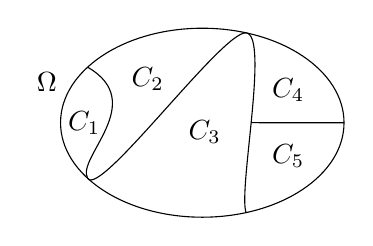
\begin{tikzpicture}[scale=.6]
			\draw (0,0) ellipse[x radius=3cm, y radius=2cm];
			\foreach \i in {1,...,5} \path ({360/5*\i}:3cm and 2cm) coordinate (A\i);
			\path (-2.5,0) node {$C_1$};
			\path (130:0.6*3cm and 0.6*2cm) node {$C_2$};
			\path (280:0.1*3cm and 0.1*2cm) node {$C_3$};
			\path (30:0.7*3cm and 0.7*2cm) node {$C_4$};
			\path (-30:0.7*3cm and 0.7*2cm) node {$C_5$};
			\draw[name path=curve]
			(A4)
			.. controls +(110:0.5) and +(-5:0.5) ..
			(A1)
			.. controls +(175:0.5) and +(-60:0.5) ..
			(A3)
			.. controls +(120:0.5) and +(-30:1.5) ..
			(A2);
			\path[name path=line] (0,0) -- (3,0);
			\path[name intersections={of=curve and line, by=Z}];
			\draw (Z) -- (3,0);
			\path (160:3cm and 2cm) coordinate (A);
			\path (A) ++(160:.5cm) node (omega) {$\Omega$};
		\end{tikzpicture}
	\end{columns}
	\vspace{5pt}
	{\bf\underline{The law of total probability}} \par
	If $\lbrace C_i\rbrace_{i=1}^n$ is a partition of $\Omega$, then:
	\begin{eqnarray*}
		P(A)&=&\sum_{i=1}^nP(A\cap C_i)\\
		&=&\sum_{i=1}^nP(A\vert C_i)P(C_i)
	\end{eqnarray*}
	{\small\color{NavyBlue} - we can derive this from the axioms of probability.  
		- this rule is very useful, especially when stated in terms of conditional probability.}
\end{frame}

\begin{frame}
	\frametitle{Independence}
	{\bf\underline{Definition}} \par
	Events $A$ and $B$ are independent if information about $A$ does not affect uncertainty about $B$. \par
	Formally, $A$ and $B$ are independent if:
	$$P(A\vert B)=P(A).$$
	Note: $P(A\cap B)=P(A\vert B)P(B)$, so independence is equivalent to
	$$P(A\cap B)=P(A)P(B).$$
	A set of events $X_1,X_2,\dots,X_n$ are mutually independent if: \par 
	for all subsets $\{X_{i_1},X_{i_2},\dots,X_{i_k}\}$ of $\{X_1,X_2,\dots,X_n\}$, we have
	$$P(X_{i_1}\cap X_{i_2}\cap\dots\cap X_{i_k})=P(X_{i_1})P(X_{i_2})\dots P(X_{i_k}).$$
	{\bf Question:} what does independence look like on a Venn diagram?
\end{frame}

\begin{frame}{Example 2C: pairwise independence but not mutual independence}
	\textbf{Experiment:} Toss two fair coins. Sample space
	\[
	\Omega = \{HH, HT, TH, TT\}, \quad P(\omega)=\tfrac14\ \forall \omega\in\Omega.
	\]
	
	Define events
	\begin{eqnarray}
		A &=& \{HH, HT\} \quad (\text{first toss is H}),\nonumber\\
		B &=& \{HH, TH\} \quad (\text{second toss is H}),\nonumber\\
		C &=& \{HH, TT\} \quad (\text{both tosses the same}).\nonumber
	\end{eqnarray}
	
	\begin{itemize}
		\item Each event has probability $\mathbb{P}(A)=\mathbb{P}(B)=\mathbb{P}(C)=\tfrac12$.
		\item We will show $A,B,C$ are pairwise independent but not mutually independent.
	\end{itemize}
\end{frame}

\begin{frame}{Example 2C: pairwise independence but not mutual independence}
	\textbf{Pairwise independence:}
	\[
	A \cap B = \{HH\}, \quad \mathbb{P}(A \cap B) = \tfrac14 = \tfrac12 \cdot \tfrac12 = \mathbb{P}(A)\mathbb{P}(B),
	\]
	\[
	A \cap C = \{HH\}, \quad \mathbb{P}(A \cap C) = \tfrac14 = \mathbb{P}(A)\mathbb{P}(C),
	\]
	\[
	B \cap C = \{HH\}, \quad \mathbb{P}(B \cap C) = \tfrac14 = \mathbb{P}(B)\mathbb{P}(C).
	\]
	So $A,B,C$ are pairwise independent.
	
	\bigskip
	\textbf{Not mutually independent:}
	\[
	A \cap B \cap C = \{HH\} \quad \Rightarrow \quad \mathbb{P}(A \cap B \cap C) = \tfrac14.
	\]
	But
	\[
	\mathbb{P}(A)\mathbb{P}(B)\mathbb{P}(C) = \tfrac12 \cdot \tfrac12 \cdot \tfrac12 = \tfrac18 \neq \tfrac14.
	\]
	\alert{Conclusion:} pairwise independence does \emph{not} imply mutual independence.
\end{frame}



\begin{frame}
	\frametitle{What is probability?}
	{\bf\underline{Frequentist definition}} \par
	Probability is the long-run relative frequency of an event occurring when an experiment is repeated under identical conditions:
	$$P(A)=\lim_{n\rightarrow\infty}\frac{k_n(A)}n,$$
	where $k_n(A)$ denotes the observed number of occurrences of $A$ in $n$ trials. \par
	{\small\color{NavyBlue} - here it is objective and based on observed data: each event has a true, fixed parameter defining its probability.  
		- the remainder of MATH163 will assume the frequentist interpretation of probability.} \par
	{\bf\underline{Bayesian definition}} \par
	Probability represents a degree of belief or certainty about an event, updated as new evidence is observed. Recall:
	$$P(\theta\vert D)=\frac{P(D\vert\theta)P(\theta)}{P(D)},$$
	where $P(\theta\vert D)$ is the updated probability of a parameter $\theta$ given data $D$. \par
	{\small\color{NavyBlue} - you will still need to understand and use Bayes' rule in MATH163!}
\end{frame}

\begin{frame}
	\frametitle{$\bigstar$ Recap: rules of probability}
	Let $\Omega$ be an event space and $A,B\subseteq \Omega$, and let $\lbrace C_i\rbrace_{i=1}^n$ be a partition of $\Omega$. Then:
	\begin{eqnarray}
		&&P(\overline A)=1-P(A)\\
		&&P(\emptyset)=0\\
		&&A\subseteq B\Rightarrow P(A)\leq P(B)\\
		&&P(A\cup B)=P(A)+P(B)-P(A\cap B)\\
		&&P(A)=\sum_{i=1}^nP(A\cap C_i)=\sum_{i=1}^nP(A\vert C_i)P(C_i)\\
		&&P(A\vert B)=\frac{P(B\vert A)P(A)}{P(B)}
		=\frac{P(B\vert A)P(A)}{P(B\vert A)P(A)+P(B\vert\overline A)P(\overline A)}
	\end{eqnarray}
	Note:
	\begin{itemize}
		\item $A$ and $B$ are mutually exclusive if $P(A\cap B)=0$.  
		$\Rightarrow P(A\cup B)=P(A)+P(B)$.
		\item $A$ and $B$ are independent if $P(A\vert B)=P(A)$.  
		$\Rightarrow P(A\cap B)=P(A)\times P(B)$.
	\end{itemize}
\end{frame}

\begin{frame}
	\frametitle{$\bigstar$ How to answer questions}
	It's easy to get in a tangle when answering exam questions about probability \par
	– just like it's easy to misinterpret probabilities in the real world. \par
	Here is a step-by-step guide to approach a probability problem:
	\begin{enumerate}
		\item Label all events of interest, \par
		e.g.\ ``true +", ``true -", ``test +", ``test -". \par
		{\small\color{NavyBlue} - they need not be mutually exclusive or independent.}
		\item Write down what you know in the language of probability, \par
		e.g.\ $P(\text{test +}\vert \text{true -})=0.2$. \par
		{\small\color{NavyBlue} - be careful to get the conditional the right way round!}
		\item Write down what you want to know, e.g.\ $P(\text{true +}\vert \text{test +})$.
		\item Use only the rules of probability provided to calculate what you want to know using what you have been given (e.g.\ apply Bayes' rule).
	\end{enumerate}
	{\small\color{NavyBlue} - this seems obvious, but it's REALLY easy to jump ahead and get in a tangle.}
\end{frame}

\begin{frame}
	\frametitle{Example 2A (answer)}
	{\small
		\begin{enumerate}
			\item Labels: ``true +", ``true -", ``test +", ``test -".
			\item $0.00015$ of the female population is estimated to develop cancer per year: $P(\text{true } +)=0.00015$. \par
			$12$ million women underwent annual screening: $n=1.2\times 10^7$. \par
			False positive rate $20\%$: $P(\text{test } +\vert \text{true } -)=0.2$. \par
			False negative rate $5\%$: $P(\text{test } -\vert \text{true } +)=0.05$.
			\item We want to know: $P(\text{true } +\vert \text{test } +)$.
			\item Apply the rules:
			\begin{eqnarray*}
				P(\text{true } +\vert \text{test } +)
				&=&\frac{P(\text{test } +\vert \text{true } +)\,P(\text{true } +)}
				{P(\text{test } +)}\quad\text{(Bayes' rule)}\\
				P(\text{test } +)
				&=&P(\text{test } +\vert \text{true } -)P(\text{true } -)
				+P(\text{test } +\vert \text{true } +)P(\text{true } +)\\
				\text{so}\quad
				P(\text{true } +\vert \text{test } +)
				&=&\frac{0.95\times 0.00015}{0.2\times 0.99985+0.95\times 0.00015}\\
				&\approx&0.00071.
			\end{eqnarray*}
			This is $0.071\%$.
		\end{enumerate}
	}
	{\small\color{NavyBlue} - by the law of total probability, the denominator in Bayes' rule is a sum, and the numerator is one of the terms in the sum.  
		- we didn't need to use all of the information that was given in order to answer the question!} \par
	{\bf Question:} what percentage of women who tested negative were true positives?
\end{frame}

\begin{frame}
	\frametitle{Example 2A (answer)}
	Why is this so confusing? \par
	{\bf Mistake:} \par
	``A $20\%$ false positive rate means if I test positive I'm $80\%$ likely to have the disease." \par
	{\bf Truth:} \par
	``A $20\%$ false positive rate means that $20\%$ of the true negatives will test positive." \par
	{\small\color{NavyBlue} - the proportion of true negatives testing positive depends on the proportion of true positives in the population!} \par
	
	\tikzstyle{box}=[draw, minimum width=5em, 
	text centered, minimum height=2.5em, line width=1.5pt]
	\begin{center}
		\begin{tikzpicture}[node distance=0cm,outer sep = 0pt]
			\node (A) [box,text width=15em,text height=6em] {};
			\node (B) [box,below= of A.east,anchor=west,text width=6em,text height=6em,fill=red!30] {};
			\node (C) [box,below= of A.south,anchor=north,text width=15em,fill=NavyBlue!30] {};
			\node (D) [box,below= of B.south,anchor=north,text width=6em,fill=black!60] {};
			\node (1) [below= of A.north,anchor=south] {true -};
			\node (2) [below= of B.north,anchor=south] {true +};
			\node (3) [left= of A.west,anchor=east] {test -};
			\node (4) [left= of C.west,anchor=east] {test +};
		\end{tikzpicture}
	\end{center}
	
	{\bf Question:} what percentage of women who tested negative were true positives?
\end{frame}

\begin{frame}
	\frametitle{Example 2C}
	You are dealt a poker hand ($5$ cards from one deck). What is the probability of drawing at least one king? \par
	\vspace{5pt}
	\includegraphics[width=\textwidth]{cards.png} \par
	\vspace{5pt}
	{\small\color{NavyBlue} Hint: a simpler route is often to compute  
		$P(\text{at least one king}) = 1 - P(\text{no kings})$.  
		This can be done without considering successive draws as separate random variables.}
\end{frame}

\begin{frame}
	\frametitle{Example 2D}
	Traffic accidents are known to be influenced by weather conditions. Suppose the probability of a traffic accident on a given day depends on whether the day is sunny or rainy. Assume that:
	\begin{itemize}
		\item $70\%$ of days are sunny (so $30\%$ are rainy),
		\item on sunny days, $5\%$ have traffic accidents,
		\item on rainy days, $15\%$ have traffic accidents.
	\end{itemize}
	You work for the emergency services in a room with no windows. You get a call reporting a traffic accident. \par
	\vspace{3pt}
	\begin{enumerate}[(a)]
		\item What is the probability that today is rainy?
		\item You have not seen a weather forecast. What is the probability of an accident occurring tomorrow?
		\item What assumptions have been made in your calculations?
	\end{enumerate}
	
	\begin{center}
		\fbox{\includegraphics[width=.2\textwidth]{countdown.jpg}}
	\end{center}
\end{frame}


% ============================================================
% Week 3
% ============================================================

\section{Week 3: transforming random variables}

\begin{frame}
	\frametitle{Recap: random variables}
	A random variable describes the outcome of an experiment \emph{before} it has been observed. \par
	The {\bf event space} $\Omega_X$ of a random variable $X$ is the set of possible outcomes. \par
	Random variables can be:
	\begin{itemize}
		\item {\bf Discrete:} the outcome space is finite or countably infinite \par
		(typically $\Omega_X\subseteq\mathbb Z$)
		\item {\bf Continuous:} the outcome space is uncountably infinite \par
		(typically $\Omega_X=(a,b),\ (0,\infty)$ or $\mathbb R$)
	\end{itemize}
	A random variable is fully characterised by its outcome space and the corresponding probabilities. \par
	More formally, a random variable is characterised by a probability space.
\end{frame}

\begin{frame}
	\frametitle{Recap: discrete vs continuous}
	Discrete random variables are characterised by {\bf probability mass functions (PMFs)}. \par
	If $X$ is a discrete random variable with PMF $p_X(x)$ and event space $\Omega_X$, then:
	\begin{eqnarray*}
		P(X=k)&=&p_X(k)\\
		\sum_{k\in\Omega_X}p_X(k)&=&1\\
		p_X(x)&\geq&0 \quad \forall x\in\Omega_X
	\end{eqnarray*}
	Continuous random variables are characterised by {\bf probability density functions (PDFs)}. \par
	If $Y$ is a continuous random variable with PDF $f_Y(y)$ and event space $\Omega_Y$, then:
	\begin{eqnarray*}
		P(Y\in(a,b))&=&\int_a^b f_Y(y)\,dy\\
		\int_{-\infty}^{\infty} f_Y(y)\,dy&=&1\\
		f_Y(y)&\geq&0 \quad \forall y\in\Omega_Y
	\end{eqnarray*}
	- A single value of a PDF is not a probability (hence ``density'' rather than ``mass'').
\end{frame}

\begin{frame}
	\frametitle{Recap: cumulative distribution}
	{\bf Cumulative distribution functions (CDFs)} can be defined for all random variables:
	\begin{eqnarray*}
		F_X(x)&:=&P(X\leq x)=\sum_{k\leq x}p_X(k)\\
		F_Y(y)&:=&P(Y\leq y)=\int_{-\infty}^y f_Y(t)\,dt
	\end{eqnarray*}
	Useful results:
	\begin{eqnarray*}
		P(X=x)&=&\lim_{z\rightarrow x^+}F_X(z)-\lim_{z\rightarrow x^-}F_X(z)\\
		P(Y\in(a,b))&=&F_Y(b)-F_Y(a)\\
		f_Y(y)&=&\frac{d}{dy}F_Y(y)\\
		f_Y(y)\geq 0\ \forall y\in\mathbb R &\Leftrightarrow& F_Y(y)\ \text{is monotone increasing}
	\end{eqnarray*}
	Random variables can also be fully characterised by their CDF.
\end{frame}

\begin{frame}
	\frametitle{Recap: mean and variance}
	{\bf\underline{Mean / expectation}}
	\begin{eqnarray*}
		E[X]&:=&\sum_{x\in\Omega_X} x\,p_X(x)\\
		E[Y]&:=&\int_{-\infty}^{\infty} y\,f_Y(y)\,dy
	\end{eqnarray*}
	{\bf\underline{Variance}}
	\begin{eqnarray*}
		\mathrm{Var}(X)&:=&\sum_{x\in\Omega_X} (x-E[X])^2 p_X(x)\\
		&=&\sum_{x\in\Omega_X} x^2 p_X(x)-E[X]^2\\
		&=&E[X^2]-E[X]^2\\[3pt]
		\mathrm{Var}(Y)&:=&\int_{-\infty}^{\infty} (y-E[Y])^2 f_Y(y)\,dy\\
		&=&\int_{-\infty}^{\infty} y^2 f_Y(y)\,dy - E[Y]^2\\
		&=&E[Y^2]-E[Y]^2
	\end{eqnarray*}
	{\small\color{NavyBlue} There is a sneaky transformed random variable in here: $X^2$ or $Y^2$.}
\end{frame}

\begin{frame}
	\frametitle{Equality between random variables}
	Let $X$ and $X'$ be two random variables. \par
	Equality between random variables can be established in two different ways:
	\begin{itemize}
		\item {\bf Equality in distribution:} $X\stackrel{d}{=}X'$ \par
		$X$ and $X'$ follow the same distribution, i.e.\ are defined by the same PMF/PDF/CDF. \par
		Example: rolling a die, and picking a card from $\{A\clubsuit,2\clubsuit,3\clubsuit,4\clubsuit,5\clubsuit,6\clubsuit\}$.
		\item {\bf Equality of variables:} $X=X'$ \par
		The realised outcome of $X$ is equal to the realised outcome of $X'$. \par
		Example: you roll a die, and whichever number you roll is the number of pounds you win. ``Die outcome'' and ``prize money'' are equal.
	\end{itemize}
\end{frame}

\begin{frame}
	\frametitle{Functions of random variables}
	Let $X$ be a random variable with sample space (outcome space) $\Omega_X$ and let $G:\Omega_X\rightarrow\Omega_Y$ be a function. \par
	We can define a new random variable $Y=G(X)$ such that outcome $x$ of $X$ is mapped to $y=G(x)$. \par
	Given a PMF or PDF for $X$, we often want to know the corresponding PMF or PDF of $Y=G(X)$. \par
	{\bf This is NOT the same as} $p_Y(y)=G(p_X(x))$. \par
	In the discrete case, deriving the PMF of $Y$ is a matter of ``bookkeeping'':
	$$P(Y=k)=\sum_{\{x:\,G(x)=k\}} p_X(x).$$
	{\small\color{NavyBlue} Count the different outcomes of $X$ that map to $k$, and add up their probabilities.} \par
	Note: we use capital letters for random variables ($V,W,X,Y,Z$), and capital letters ($F,G,H$) for functions of random variables, since a function of a random variable is itself a random variable. We will avoid $F$ for functions, as $F$ is used for CDFs.
\end{frame}

\begin{frame}
	\frametitle{Example 3A}
	Simple game: you pay \pounds$A$ to enter — this is called the ante. \par
	A die is rolled once. If you roll $1,2$ or $3$, you lose your money. \par
	Roll a $4$ or $5$ and win \pounds$5$; roll a $6$ and win \pounds$50$. \par
	{\bf\underline{Question}} \par
	You run the casino — what should the value of $A$ be in order for the game to make a profit?
\end{frame}

\begin{frame}
	\frametitle{Example 3A}
	{\bf\underline{Answer}} \par
	Let $X$ be a random variable describing the outcome of rolling a die: $\Omega_X=\{1,2,3,4,5,6\}$. \par
	Let $Y$ be the amount of money won (not including the ante): $\Omega_Y=\{0,5,50\}$. \par
	We have $Y=G(X)$ where:
	$$
	p_X(x) = \left\{\begin{array}{ll}
		\dfrac 16, & x=1,2,3,4,5,6\\[3pt]
		0, & \text{otherwise}
	\end{array}\right.,
	\qquad
	G(x)=\left\{\begin{array}{ll}
		5, & x\in\{4,5\}\\
		50, & x=6\\
		0, & \text{otherwise}
	\end{array}\right.
	$$
	From this we can calculate:
	$$
	p_Y(y) = \left\{\begin{array}{ll}
		\dfrac 16, & y=50\\[3pt]
		\dfrac 13, & y=5\\[3pt]
		\dfrac 12, & y=0\\[3pt]
		0, & \text{otherwise}
	\end{array}\right.
	$$
	{\small\color{gray}Recall: $P(Y=k)=\sum_{\{x:\,G(x)=k\}} p_X(x)$.} \par
	{\bf Warning:} do not confuse an outcome $0$ with an outcome occurring with probability $0$.
\end{frame}

\begin{frame}
	\frametitle{Example 3A}
	{\bf\underline{Answer (continued)}} \par
	In order for the casino to turn a profit, we need $A>E[Y]$:
	\begin{eqnarray*}
		E[Y]&=&\sum_y y\,p_Y(y)\\
		&=&\frac 16\times 50+\frac 13\times 5\\
		&=&10.
	\end{eqnarray*}
	So pick $A>10$ — what can we get away with?
\end{frame}

\begin{frame}
	\frametitle{Transforming discrete random variables: mean}
	If $Y=G(X)$ then:
	\begin{eqnarray*}
		E[Y]&:=&\sum_y y\,P(Y=y)\\
		&=&\sum_y y\sum_{\{x:\,G(x)=y\}} P(X=x)\\
		&=&\sum_x G(x)P(X=x)\\
		&=&\sum_x G(x)\,p_X(x).
	\end{eqnarray*}
	{\small\color{NavyBlue} For each $y$, sum over the $x$'s that map to $y$, or simply sum over all $x$.} \par
	{\bf\underline{Question}} \par
	If $Y=G(X)$, can we say $E[Y]=G(E[X])$?
\end{frame}

\begin{frame}
	\frametitle{Transforming discrete random variables: mean}
	{\bf\underline{Answer}} \par
	If $Y=mX+c$ then:
	\begin{eqnarray*}
		E[Y]&=&\sum_x (mx+c)p_X(x)\\
		&=&m\sum_x x p_X(x)+c\sum_x p_X(x)\\
		&=&mE[X]+c.
	\end{eqnarray*}
	- this is the {\bf linearity} property of expectation. \par
	Likewise, if $Y=mG(X)+c$ then:
	$$E[Y]=mE[G(X)]+c.$$
	BUT consider $Y=X^2$. Then
	$$E[Y]=E[X^2]=\mathrm{Var}(X)+E[X]^2,$$
	so in general $E[Y]\neq G(E[X])=E[X]^2$ unless $\mathrm{Var}(X)=0$.
\end{frame}

\begin{frame}
	\frametitle{Transforming discrete random variables: variance}
	If $Y=G(X)$ then:
	\begin{eqnarray*}
		\mathrm{Var}(Y)&:=&E[Y^2]-E[Y]^2\\
		&=&\sum_x G(x)^2 p_X(x) - \left(\sum_x G(x)p_X(x)\right)^2.
	\end{eqnarray*}
	{\bf\underline{Question}} \par
	If $Y=G(X)$, can we say $\mathrm{Var}(Y)=G(\mathrm{Var}(X))$? \par
	What if $G(X)=mX+c$?
\end{frame}

\begin{frame}
	\frametitle{Transforming discrete random variables: variance}
	If $Y=mX+c$ then:
	\begin{eqnarray*}
		\mathrm{Var}(Y)
		&=&\sum_x (mx+c)^2 p_X(x)-E[mX+c]^2\\
		&=&\sum_x (m^2x^2+2mcx+c^2)p_X(x)-(mE[X]+c)^2\\
		&=&m^2E[X^2]+2mcE[X]+c^2 - m^2E[X]^2-2mcE[X]-c^2\\
		&=&m^2\mathrm{Var}(X).
	\end{eqnarray*}
	Likewise, if $Y=mG(X)+c$ then:
	$$\mathrm{Var}(Y)=m^2\,\mathrm{Var}\big(G(X)\big).$$
	{\bf Corollary:} adding a constant to a random variable does not change its variance.
\end{frame}

\begin{frame}
	\frametitle{Example 3B}
	Let $X$ be a random variable representing the magnitude of an earthquake on the Richter scale in a specific region. We know:
	$$P(X=3)=0.2,\quad P(X=4)=0.3,\quad P(X=5)=0.3,\quad P(X=6)=0.2.$$
	Let $Y$ denote the economic cost of an earthquake based on its magnitude:
	$$Y=G(X)=\frac {L}{1+e^{-k(X-X_0)}},$$
	where:
	\begin{itemize}
		\item $L=10{,}000$ is the maximum possible damage in \pounds millions,
		\item $X_0=5$ is the magnitude at which damage reaches half of the maximum,
		\item $k=1.5$ controls the steepness of the curve.
	\end{itemize}
	Note: all of this is conditional on the event that an earthquake occurs.
\end{frame}

\begin{frame}
	\frametitle{Example 3B}
	{\bf\underline{Questions}} \par
	\begin{itemize}
		\item Compute $E[X]$ and $\mathrm{Var}(X)$.
		\item Write down the PMF of $Y$.
		\item Compute $E[Y]$ and $\mathrm{Var}(Y)$.
		\item The energy released in an earthquake is modelled as $E=E_0\times 10^{1.5X}$, where $E_0$ is the reference energy (magnitude $0$). Explain why we do not use this exponential transformation to model economic cost.
	\end{itemize}
	\begin{center}
		\fbox{\includegraphics[width=.2\textwidth]{countdown.jpg}}
	\end{center}
	Hint: sketch the function $y=G(x)$ as a continuous curve first, even though $X$ is discrete.
\end{frame}

\begin{frame}
	\frametitle{Example 3C: Lotto}
	Disclaimer: this example brings together combinatorics, probability and transformed random variables. It is more involved than any single assessment question. \par
	The rules of Lotto:
	\begin{itemize}
		\item A single ticket costs \pounds$2$.
		\item You pick $6$ distinct numbers between $1$ and $59$.
		\item $6$ main balls are drawn from a set numbered $1$–$59$, plus one bonus ball (BB).
		\item You win money if your numbers match the balls, with prizes as follows:
	\end{itemize}
	\begin{table}
		\centering
		\begin{tabular}{|l|l|}
			\hline 
			Match & Prize \\ \hline
			Exactly $3$ main balls & \pounds$30$ \\
			Exactly $4$ main balls & \pounds$140$ \\
			Exactly $5$ main balls and NOT the BB & \pounds$1{,}750$ \\
			Exactly $5$ main balls + BB & \pounds$1{,}000{,}000$ \\
			All $6$ main balls & Jackpot \pounds$J$ \\ \hline
		\end{tabular}
	\end{table}
\end{frame}

\begin{frame}
	\frametitle{Example 3C: Lotto}
	{\bf\underline{Questions}} \par
	\begin{itemize}
		\item What is the expected win on a single lottery ticket (in terms of $J$)?
		\item How large would the jackpot have to be for the lottery to be lucrative for players in the long run?
		\item $N$ tickets are sold. Write an equation describing the expected gross profit made from the lottery in terms of $N$ and $J$.
	\end{itemize}
\end{frame}

\begin{frame}
	\frametitle{Example 3C: Lotto}
	We \emph{could} fix our ticket numbers and view the lottery draw as the random variable. \par
	Equivalently, we could fix the draw numbers and view our ticket selection as a random variable.
	\begin{itemize}
		\item If $X$ represents your number selection, then $\Omega_X$ is the set of all $6$-element subsets of $\{1,2,\dots,59\}$.
		\item $X$ follows a discrete uniform distribution.
		\item Let $Y=G(X)$ denote the prize for line $X$.
		\item A lottery line is a set of numbers. Order does not matter — it is therefore common practice to list numbers in numerical order.
	\end{itemize}
\end{frame}

\begin{frame}
	\frametitle{Example 3C: Lotto}
	Start by asking: how many ways are there for my ticket to match the lottery draw in each winning category?
	\begin{table}
		\centering
		\begin{tabular}{|l|c|c|}
			\hline 
			Match & Calculation & Value \\ \hline
			$3$ main & $\binom{6}{3}\binom{53}{3}$ & $468{,}520$ \\
			$4$ main & $\binom{6}{4}\binom{53}{2}$ & $20{,}670$ \\
			$5$ main, not BB & $\binom{6}{5}\binom{53}{1}\frac{52}{53}$ & $312$ \\
			$5$ main + BB & $\binom{6}{5}\binom{53}{1}\frac{1}{53}$ & $6$ \\
			All $6$ main balls & $\binom{6}{6}$ & $1$ \\ \hline
		\end{tabular}
	\end{table}
	(Note that $\binom{53}{52}=\binom{53}{1}$ and $\frac{1}{53}$ is the chance of hitting the BB.) \par
	Now ask: how many distinct ticket possibilities are there?
	$${59\choose 6}=45{,}057{,}474.$$
\end{frame}

\begin{frame}
	\frametitle{Example 3C: Lotto}
	Putting it all together:
	\begin{table}
		\centering
		\begin{tabular}{|l|c|c|}
			\hline 
			Event ($A\subseteq\Omega_X$) & Combinations ($|A|$) & Prize ($y$) \\ \hline
			$3$ main & $468{,}520$ & $30$\\
			$4$ main & $20{,}670$ & $140$\\
			$5$ main, not BB & $312$ & $1{,}750$\\
			$5$ main + BB & $6$ & $1{,}000{,}000$\\
			All $6$ main balls & $1$ & $J$ \\ \hline
		\end{tabular}
	\end{table}
	and $|\Omega_X|=45{,}057{,}474$. \par
	Let $A_y:=\{x\in\Omega_X: G(x)=y\}$. Then:
	\begin{eqnarray*}
		P(Y=y)&=&\frac{|A_y|}{|\Omega_X|},\\[3pt]
		E[Y]&=&\sum_y y\,P(Y=y)
		=\frac 1{|\Omega_X|}\sum_y y\,|A_y|\\
		&=&\frac J{45{,}057{,}474}+\dots
	\end{eqnarray*}
\end{frame}

\begin{frame}
	\frametitle{Example 3C: Lotto}
	{\bf\underline{Answers}} \par
	\begin{itemize}
		\item Expected win on a single lottery ticket (in terms of $J$):
		\[
		\boxed{E[Y]=\pounds\left(\frac{J}{45{,}057{,}474}+0.521454\right)}
		\]
		\item For the lottery to be lucrative for players we require $E[Y]>2$:
		\[
		\frac{J}{45{,}057{,}474}+0.521454>2
		\quad\Rightarrow\quad
		J>(2-0.521454)\times 45{,}057{,}474
		\approx \boxed{\pounds 66{,}619{,}548}.
		\]
		\item If $N$ tickets are sold, the expected gross profit of the lottery is
		\[
		\text{profit}=2N - N E[Y]
		=\pounds N\left(1.478546-\frac{J}{45{,}057{,}474}\right).
		\]
		(This uses linearity of expectation from Week 4.)
	\end{itemize}
\end{frame}

\begin{frame}
	\frametitle{Example 3D: transforming continuous random variables}
	But what if $X$ is a continuous random variable? \par
	%{\bf\underline{Example 3D} 
	(solved later) \par 
	We observe that the time taken to drive $1$ km on a motorway is (approximately) uniformly distributed between $40$ and $60$ seconds. \par
	We have $T\sim \mathrm{Unif}(40,60)$ and define $X=\dfrac 1T$ (average speed in km/s). \par 
	What is the distribution of $X$?
\end{frame}

\begin{frame}[t]
	\frametitle{$\bigstar$ Example 3E: transforming continuous random variables}
	{\small
		\begin{minipage}{\textwidth}
			\begin{columns}[T]
				\column{0.17\textwidth}
				\column{0.35\textwidth}
				\underline{General case} \par
				$Z=G(X)$, $f_X(x)$ known
				\column{0.4\textwidth}
				\underline{Example 3E} \par
				$Z=X^2+1,\ f_X(x)=e^{-x},\ x\geq 0$
			\end{columns}
		\end{minipage}\par
		\begin{minipage}{\textwidth}
			\begin{columns}[T]
				\column{0.17\textwidth}
				\underline{Step 1} \par
				Compute CDF of $X$
				\column{0.35\textwidth}
				\hfill\break\hfill\break
				$F_X(x)=P(X\leq x)$
				\column{0.4\textwidth}
				\hfill\break\hfill\break
				$F_X(x)=\int_0^x e^{-t}\,dt
				=1-e^{-x},\ x\ge 0$
			\end{columns}
		\end{minipage}\par
		\begin{minipage}{\textwidth}
			\begin{columns}[T]
				\column{0.17\textwidth}
				\underline{Step 2} \par
				Write $F_Z(z)$ in terms of $X$
				\column{0.35\textwidth}
				\hfill\break\hfill\break
				$P(Z\leq z)=P(G(X)\leq z)$
				\column{0.4\textwidth}
				\hfill\break\hfill\break
				$P(Z\leq z)=P(X^2+1\leq z)$
			\end{columns}
		\end{minipage}\par
		\begin{minipage}{\textwidth}
			\begin{columns}[T]
				\column{0.17\textwidth}
				\underline{Step 3} \par
				Rearrange the inequality in terms of $X$
				\column{0.35\textwidth}
				\hfill\break\hfill\break
				$P(Z\leq z)=P(X\leq G^{-1}(z))$
				\column{0.4\textwidth}
				\hfill\break\hfill\break
				$P(Z\leq z)=P(X\leq \sqrt{z-1})$
			\end{columns}
		\end{minipage}\par
		\begin{minipage}{\textwidth}
			\begin{columns}[T]
				\column{0.17\textwidth}
				\underline{Step 4} \par
				Substitute CDF of $X$
				\column{0.35\textwidth}
				\hfill\break\hfill\break
				$F_Z(z)=F_X(G^{-1}(z))$
				\column{0.4\textwidth}
				\hfill\break\hfill\break
				$F_Z(z)= 1-e^{-\sqrt{z-1}},\quad z>1$
			\end{columns}
		\end{minipage}\par
		\begin{minipage}{\textwidth}
			\begin{columns}[T]
				\column{0.17\textwidth}
				\underline{Step 5} \par
				Differentiate w.r.t.\ $z$
				\column{0.35\textwidth}
				\hfill\break\hfill\break
				$f_Z(z)=\dfrac{d}{dz}F_Z(z)$
				\column{0.4\textwidth}
				\hfill\break\hfill\break
				$f_Z(z)=\dfrac{d}{dz}\big(1-e^{-\sqrt{z-1}}\big)$ \par
				$\qquad\ \ =\dfrac{1}{2\sqrt{z-1}}e^{-\sqrt{z-1}},\quad z>1.$ \par
				\color{NavyBlue}{\tiny - please do check this!}
			\end{columns}
		\end{minipage}\par
	}
	Warning: upper case letters denote random variables and lower case letters specific values.
\end{frame}

\begin{frame}
	\frametitle{Example 3D (revisited)}
	$T\sim \mathrm{Unif}(40,60)$ and $X=\dfrac 1T$. \par
	{\bf\underline{Questions}}
	\begin{itemize}
		\item What is the PDF of $X$?
		\item What are the limitations of this method?
	\end{itemize}
\end{frame}

\begin{frame}
	\frametitle{Example 3D (revisited)}
	{\bf\underline{Answers}} \par
	\begin{enumerate}
		\item $F_T(t)=\dfrac{t-40}{20},\quad t\in[40,60]$.
		\item $F_X(x)=P\!\left(\frac 1T\leq x\right)$.
		\item $F_X(x)=P\!\left(T\geq \frac 1x\right)=1-P\!\left(T\leq\frac 1x\right),\quad x\in\left[\frac 1{60},\frac 1{40}\right].$
		\item $F_X(x) =1-\dfrac 1{20}\left(\frac 1x-40\right)=3-\frac{1}{20x}$.
		\item $f_X(x)=\dfrac{d}{dx}\!\left[3-\frac{1}{20x}\right]=\dfrac{1}{20x^2},\quad x\in\left[\frac 1{60},\frac 1{40}\right].$
	\end{enumerate}
	Limitation: we need $G$ to be one-to-one on the support of $X$ so that $G^{-1}$ is well defined.
\end{frame}

\begin{frame}
	\frametitle{Example 3F}
	{\bf\underline{Exercise}} \par
	A continuous random variable $X$ is uniformly distributed on the interval $\big(0,\frac{\pi}2\big)$. \par
	Let $Y=\sin(X)$.
	\begin{itemize}
		\item Find the PDF of $Y$.
		\item Sketch the PDFs of $X$ and $Y$.
	\end{itemize}
	\begin{center}
		\fbox{\includegraphics[width=.2\textwidth]{countdown.jpg}}
	\end{center}
	Hint: you may need to look up a bit of calculus. \par
	This question is here to show you that the answer may not be what you expect.
	
	\begin{center}
		\fbox{\includegraphics[width=.2\textwidth]{countdown.jpg}}
	\end{center}
\end{frame}

\begin{frame}
	\frametitle{Transforming continuous random variables: mean}
	If $Y=mX+c$ then:
	\begin{eqnarray*}
		E[Y]&=&\int_{-\infty}^{\infty} (mx+c)\,f_X(x)\,dx\\
		&=&m\int x f_X(x)\,dx + c\int f_X(x)\,dx\\
		&=&mE[X]+c.
	\end{eqnarray*}
	- this is the {\bf linearity} property of expectation. \par
	Likewise, if $Y=mG(X)+c$ then:
	$$E[Y]=mE[G(X)]+c.$$
	{\bf This is exactly the same result as for the discrete case.}
\end{frame}

\begin{frame}
	\frametitle{Transforming continuous random variables: variance}
	If $Y=G(X)$, then:
	\begin{eqnarray*}
		\mathrm{Var}(Y)
		&=&E[Y^2]-E[Y]^2\\
		&=&\int_{-\infty}^{\infty} G(x)^2 f_X(x)\,dx
		-\left(\int_{-\infty}^{\infty} G(x) f_X(x)\,dx\right)^2.
	\end{eqnarray*}
	If $Y=mX+c$ then:
	\begin{eqnarray*}
		\mathrm{Var}(Y)
		&=&\int (mx+c)^2 f_X(x)\,dx - E[mX+c]^2\\
		&=&m^2E[X^2]+2mcE[X]+c^2 - m^2E[X]^2-2mcE[X]-c^2\\
		&=&m^2\mathrm{Var}(X).
	\end{eqnarray*}
	Likewise, if $Y=mG(X)+c$ then:
	$$\mathrm{Var}(Y)=m^2\,\mathrm{Var}\big(G(X)\big).$$
	{\bf Again, this matches the discrete case.}
\end{frame}


% ============================================================
% Week 4
% ============================================================

\section{Week 4: combining random variables}
% Limit laws (later in the module)

\begin{frame}
	\frametitle{Recap}
	One random variable can be a function of another, i.e.\ $Y=G(X)$. \par
	Here we apply the function $G$ to the \emph{outcome} of the random variable $X$. \par
	Classic example: outcomes from a randomised process (lottery machine) are mapped to payouts (lottery winnings). \par
	This is {\bf different} from combining distinct random variables, e.g.\ $Z=X+Y$. \par
	In reality, we often apply functions to sums of variables, or sum functions of variables. \par
	MATH163 will introduce this idea in simple terms.
\end{frame}

\begin{frame}
	\frametitle{Combining random variables}
	In the casino game ``craps'', players roll two dice. \par
	If $X_1$ and $X_2$ are the outcomes from rolling each die, then $Y=X_1+X_2$ is a new random variable. \par
	What is the PMF of $Y$? \par
	\begin{center}
		\renewcommand{\arraystretch}{1.5}
		\setlength{\tabcolsep}{10pt}
		\begin{tabular}{c c|c|c|c|c|c|c|}
			~ & \multicolumn{7}{c}{Outcome of $X_1$} \\
			&        & \textbf{1} & \textbf{2} & \textbf{3} & \textbf{4} & \textbf{5} & \textbf{6} \\
			\cline{2-8}
			\multirow{6}{*}{\rotatebox[origin=c]{90}{\parbox[c]{2cm}{\centering Outcome of $X_2$}}}
			& \textbf{1} & \cellcolor[HTML]{FFC7C7}2  & \cellcolor[HTML]{FFDDC7}3 & \cellcolor[HTML]{FFEFC7}4 & \cellcolor[HTML]{F7FFC7}5 & \cellcolor[HTML]{D2FFC7}6 & \cellcolor[HTML]{C7FFF2}7 \\
			\cline{2-8}
			& \textbf{2} & \cellcolor[HTML]{FFDDC7}3  & \cellcolor[HTML]{FFEFC7}4 & \cellcolor[HTML]{F7FFC7}5 & \cellcolor[HTML]{D2FFC7}6 & \cellcolor[HTML]{C7FFF2}7 & \cellcolor[HTML]{C7E7FF}8 \\
			\cline{2-8}
			& \textbf{3} & \cellcolor[HTML]{FFEFC7}4  & \cellcolor[HTML]{F7FFC7}5 & \cellcolor[HTML]{D2FFC7}6 & \cellcolor[HTML]{C7FFF2}7 & \cellcolor[HTML]{C7E7FF}8 & \cellcolor[HTML]{C7C7FF}9 \\
			\cline{2-8}
			& \textbf{4} & \cellcolor[HTML]{F7FFC7}5  & \cellcolor[HTML]{D2FFC7}6 & \cellcolor[HTML]{C7FFF2}7 & \cellcolor[HTML]{C7E7FF}8 & \cellcolor[HTML]{C7C7FF}9 & \cellcolor[HTML]{E7C7FF}10 \\
			\cline{2-8}
			& \textbf{5} & \cellcolor[HTML]{D2FFC7}6  & \cellcolor[HTML]{C7FFF2}7 & \cellcolor[HTML]{C7E7FF}8 & \cellcolor[HTML]{C7C7FF}9 & \cellcolor[HTML]{E7C7FF}10 & \cellcolor[HTML]{FFC7FF}11 \\
			\cline{2-8}
			& \textbf{6} & \cellcolor[HTML]{C7FFF2}7  & \cellcolor[HTML]{C7E7FF}8 & \cellcolor[HTML]{C7C7FF}9 & \cellcolor[HTML]{E7C7FF}10 & \cellcolor[HTML]{FFC7FF}11 & \cellcolor[HTML]{FFC7C7}12 \\
			\cline{2-8}
		\end{tabular}
	\end{center}
\end{frame}

\begin{frame}
	\frametitle{Combining random variables: PMF and mean}
	For the sum of two dice, the PMF of $Y=X_1+X_2$ is:
	\begin{columns}[b]
		\column{0.6\textwidth}
		\begin{table}
			\centering
			\begin{tabular}{|c|l c|}
				$y$ & \multicolumn{2}{c|}{$P(Y=y)$} \\ \hline
				2  & $1/36$           & $\approx 0.0278$ \\ \hline
				3  & $2/36=1/18$      & $\approx 0.0556$ \\ \hline
				4  & $3/36=1/12$      & $\approx 0.0833$ \\ \hline
				5  & $4/36=1/9$       & $\approx 0.1111$ \\ \hline
				6  & $5/36$           & $\approx 0.1389$ \\ \hline
				7  & $6/36=1/6$       & $\approx 0.1667$ \\ \hline
				8  & $5/36$           & $\approx 0.1389$ \\ \hline
				9  & $4/36=1/9$       & $\approx 0.1111$ \\ \hline
				10 & $3/36=1/12$      & $\approx 0.0833$ \\ \hline
				11 & $2/36=1/18$      & $\approx 0.0556$ \\ \hline
				12 & $1/36$           & $\approx 0.0278$ \\ \hline
			\end{tabular}
		\end{table}
		\column{0.4\textwidth}
		\vspace{5pt}
		\centering
		\fbox{\includegraphics[width=\textwidth]{Catan.jpg}}\\[3pt]
		{\small What is a fair placement of scores on a Catan board?}
	\end{columns}
\end{frame}

\begin{frame}
	\frametitle{Combining random variables: mean}
	{\bf\underline{Theorem}} (not proved in MATH163) \par
	If $X_1,X_2,\dots,X_n$ are random variables with $E[X_i]<\infty$ for all $i$ and $c,m_1,\dots,m_n\in\mathbb R$, then
	\begin{eqnarray*}
		E\left[c+\sum_{i=1}^n m_i X_i\right]
		&=& c+\sum_{i=1}^n m_i E[X_i].
	\end{eqnarray*}
	More generally, if $G_1,G_2,\dots,G_n$ are functions, then
	\begin{eqnarray*}
		E\left[c+\sum_{i=1}^n m_i G_i(X_i)\right]
		&=& c+\sum_{i=1}^n m_i E\big[G_i(X_i)\big].
	\end{eqnarray*}
	{\small\color{NavyBlue} Linearity of expectation does \emph{not} require independence.} \par
	Question: what about variance?
	\[
	\mathrm{Var}\left(c+\sum_{i=1}^n m_i X_i\right)=?
	\]
\end{frame}

\begin{frame}
	\frametitle{Recap: independence of events}
	{\bf\underline{Definition}} \par
	Events $A$ and $B$ are independent if learning about one does not affect our uncertainty in the other. \par
	Formally, $A$ and $B$ are independent if
	$$P(A\mid B)=P(A).$$
	We know:
	\begin{eqnarray*}
		P(A\mid B)=P(A)
		&\Leftrightarrow& P(B\mid A)=P(B)\\
		&\Leftrightarrow& P(A\cap B)=P(A)P(B).
	\end{eqnarray*}
\end{frame}

\begin{frame}
	\frametitle{Independence of random variables}
	Important distinction: independence of events is not the same as independence of random variables. \par
	Example:
	\begin{itemize}
		\item $X$: pick a card; $Y$: pick another (without replacement).
		\item $A$: the first card is red; $B$: the second card is a queen.
	\end{itemize}
	Are $X$ and $Y$ independent? \par
	Are $A$ and $B$ independent? \par
	{\bf\underline{Definition}} \par
	Random variables $X$ and $Y$ are independent if the outcome of one does not affect the PMF/PDF of the other, i.e.
	$$P(X\in A,\ Y\in B)=P(X\in A)\,P(Y\in B)$$
	for all $A\subseteq\Omega_X$, $B\subseteq\Omega_Y$.
\end{frame}

\begin{frame}
	\frametitle{Independence: examples}
	In which of the following cases are the random variables $X$ and $Y$ (approximately) independent?
	\begin{enumerate}
		\item $X$: roll a die; $Y$: roll another die.
		\item $X$: draw a card from a deck; $Y$: draw another (without replacement).
		\item $X$: LFC score on Saturday; $Y$: LFC score the following week.
		\item $X$: delay on the 14:52 to Newcastle; $Y$: delay on the 15:52.
		\item $X$: my flu test result; $Y$: Beyoncé's flu test result.
		\item $X$: my flu test result; $Y$: Daniel Colquitt's flu test result.
	\end{enumerate}
\end{frame}

\begin{frame}
	\frametitle{Independence: key result}
	{\bf\underline{Theorem} (not proved in MATH163)} \par
	If $X_1,\dots,X_n$ are {\bf independent} random variables, then
	\[
	E[X_1\cdot X_2\cdots X_n]
	=E[X_1]\cdot E[X_2]\cdots E[X_n].
	\]
	More generally, for any functions $G_1,\dots,G_n$,
	\[
	E\big[G_1(X_1)\cdots G_n(X_n)\big]
	=E[G_1(X_1)]\cdots E[G_n(X_n)].
	\]
	{\small\color{NavyBlue} Independence is extremely useful: it allows us to factor expectations of products.}
\end{frame}

\begin{frame}
	\frametitle{Combining random variables: variance}
	{\bf\underline{Theorem}} \par
	If $X_1,\dots,X_n$ are {\bf independent} random variables with $\mathrm{Var}(X_i)<\infty$ for all $i$, and $c,m_1,\dots,m_n\in\mathbb R$, then
	\[
	\mathrm{Var}\!\left(c+\sum_{i=1}^n m_i X_i\right)
	=\sum_{i=1}^n m_i^2\,\mathrm{Var}(X_i).
	\]
	We can only sum variances in this way when the random variables are {\bf independent} — why?
\end{frame}

\begin{frame}
	\frametitle{Combining random variables: variance}
	{\bf\underline{Proof idea}} \par
	For simplicity we prove the case $X+Y$. Extending to the general case is routine. \par
	For any random variables $X$ and $Y$ with finite variances:
	\begin{eqnarray*}
		\mathrm{Var}(X+Y)
		&=&E[(X+Y)^2]-E[X+Y]^2\\
		&=&E[X^2+2XY+Y^2]-\big(E[X]+E[Y]\big)^2\\
		&=&E[X^2]+2E[XY]+E[Y^2]
		-E[X]^2-2E[X]E[Y]-E[Y]^2\\
		&=&\mathrm{Var}(X)+\mathrm{Var}(Y)
		+2\big(E[XY]-E[X]E[Y]\big).
	\end{eqnarray*}
	If $X$ and $Y$ are independent, then $E[XY]=E[X]E[Y]$ and
	\[
	\mathrm{Var}(X+Y)=\mathrm{Var}(X)+\mathrm{Var}(Y).
	\]
	Note: it is possible to have $E[XY]=E[X]E[Y]$ for {\bf dependent} variables (e.g.\ $Y=X^2$ and $X$ symmetric about $0$).
\end{frame}

\begin{frame}
	\frametitle{Covariance}
	{\bf\underline{Definition}} \par
	The {\bf covariance} of two random variables $X$ and $Y$ is
	\begin{eqnarray*}
		\mathrm{Cov}(X,Y)
		&:=&E\big[(X-E[X])(Y-E[Y])\big]\\
		&=&E[XY]-E[X]E[Y].
	\end{eqnarray*}
	{\small\color{NavyBlue} Note: if $X=Y$ then $\mathrm{Cov}(X,X)=\mathrm{Var}(X)$.} \par
	\begin{center}
		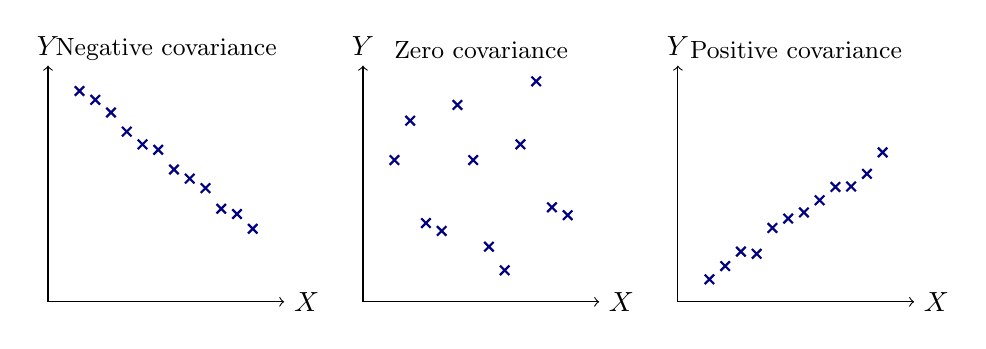
\begin{tikzpicture}
			
			% Negative Covariance Plot
			\begin{scope}[shift={(0,0)}]
				\node at (1.5, 3.2) {\small Negative covariance};
				\draw[->] (0,0) -- (3,0) node[right] {$X$};
				\draw[->] (0,0) -- (0,3) node[above] {$Y$};
				\foreach \x in {0.4, 0.8, 1.2, 1.6, 2, 2.4, 0.6, 1, 1.4, 1.8, 2.2, 2.6}
				\draw[NavyBlue, thick] (\x, {3-0.8*\x-rand/15}) +(-0.06,-0.06) -- +(0.06,0.06) +(-0.06,0.06) -- +(0.06,-0.06);
			\end{scope}
			
			% Zero Covariance Plot
			\begin{scope}[shift={(4,0)}]
				\node at (1.5, 3.2) {\small Zero covariance};
				\draw[->] (0,0) -- (3,0) node[right] {$X$};
				\draw[->] (0,0) -- (0,3) node[above] {$Y$};
				\foreach \x/\y in {0.4/1.8, 0.8/1, 1.2/2.5, 1.6/0.7, 2/2, 2.4/1.2, 0.6/2.3, 1/0.9, 1.4/1.8, 1.8/0.4, 2.2/2.8, 2.6/1.1}
				\draw[NavyBlue, thick] (\x, \y) +(-0.06,-0.06) -- +(0.06,0.06) +(-0.06,0.06) -- +(0.06,-0.06);
			\end{scope}
			
			% Positive Covariance Plot
			\begin{scope}[shift={(8,0)}]
				\node at (1.5, 3.2) {\small Positive covariance};
				\draw[->] (0,0) -- (3,0) node[right] {$X$};
				\draw[->] (0,0) -- (0,3) node[above] {$Y$};
				\foreach \x in {0.4, 0.8, 1.2, 1.6, 2, 2.4, 0.6, 1, 1.4, 1.8, 2.2, 2.6}
				\draw[NavyBlue, thick] (\x, {0.7*\x + rand/10}) +(-0.06,-0.06) -- +(0.06,0.06) +(-0.06,0.06) -- +(0.06,-0.06);
			\end{scope}
			
		\end{tikzpicture}
	\end{center}
\end{frame}

\begin{frame}
	\frametitle{Covariance and correlation}
	Covariance captures the idea of linear dependence, but $\mathrm{Cov}(X,X)=\mathrm{Var}(X)$, which is constrained only to being non-negative. \par
	{\bf\underline{Definition}} \par
	The (Pearson) {\bf correlation coefficient} of $X$ and $Y$ is
	\[
	\rho_{X,Y}:=\frac{\mathrm{Cov}(X,Y)}
	{\sqrt{\mathrm{Var}(X)}\sqrt{\mathrm{Var}(Y)}}.
	\]
	This value is constrained to the interval $[-1,1]$, with
	\[
	\rho_{X,X}=1,\qquad \rho_{X,-X}=-1.
	\]
\end{frame}

\begin{frame}
	\frametitle{Correlation and causation}
	$X$ and $Y$ are (linearly) {\bf correlated} if $\mathrm{Cov}(X,Y)\neq 0$. \par
	{\bf This does NOT mean that they are causally related.}
	\begin{center}
		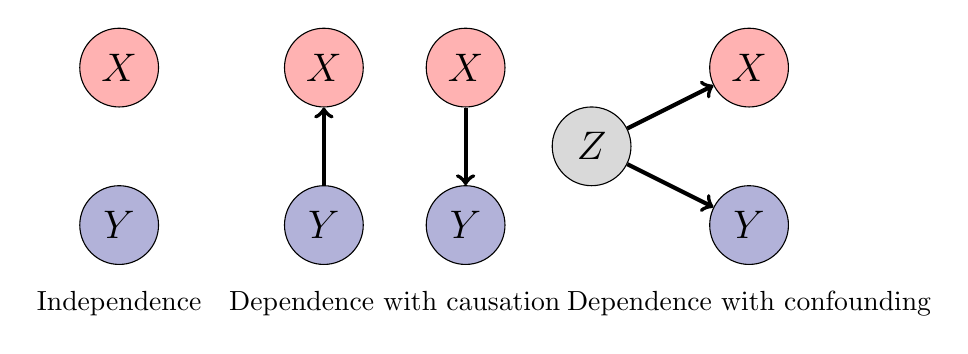
\begin{tikzpicture}[node distance=1.5cm]
			% Independence
			\node[draw,circle,fill=red!30,minimum size=1cm,align=center] (A1) at (0,0) {\Large $X$};
			\node[draw,circle,fill=NavyBlue!30,minimum size=1cm,align=center] (B1) at (0,-2) {\Large $Y$};
			
			% Direct causation Y -> X
			\node[draw,circle,fill=red!30,minimum size=1cm,align=center] (A2) at (2.6,0) {\Large $X$};
			\node[draw,circle,fill=NavyBlue!30,minimum size=1cm,align=center] (B2) at (2.6,-2) {\Large $Y$};
			\draw[->,line width=1.5pt] (B2) -- (A2);
			
			% Direct causation X -> Y
			\node[draw,circle,fill=red!30,minimum size=1cm,align=center] (A2b) at (4.4,0) {\Large $X$};
			\node[draw,circle,fill=NavyBlue!30,minimum size=1cm,align=center] (B2b) at (4.4,-2) {\Large $Y$};
			\draw[->,line width=1.5pt] (A2b) -- (B2b);
			
			% Confounding
			\node[draw,circle,fill=red!30,minimum size=1cm,align=center] (A3) at (8,0) {\Large $X$};
			\node[draw,circle,fill=NavyBlue!30,minimum size=1cm,align=center] (B3) at (8,-2) {\Large $Y$};
			\node[draw,circle,fill=gray!30,minimum size=1cm,align=center] (C3) at (6,-1) {\Large $Z$};
			\draw[->,line width=1.5pt] (C3) -- (A3);
			\draw[->,line width=1.5pt] (C3) -- (B3);
			
			% Labels
			\node[align=center] at (0,-3) {Independence};
			\node[align=center] at (3.5,-3) {Dependence with causation};
			\node[align=center] at (8,-3) {Dependence with confounding};
		\end{tikzpicture}
	\end{center}
	Consider the random variables:
	\begin{itemize}
		\item Ice cream sales
		\item Daily high temperature
		\item Daily coast guard emergencies
	\end{itemize}
	They are all correlated — but which relationships are causal?
\end{frame}

\begin{frame}
	\frametitle{Summary of combination rules}
	So far we have:
	\begin{itemize}
		\item If $Y=X+X'$ then {\bf always} $E[Y]=E[X]+E[X']$.
		\item If $Y=mX+c$ then {\bf always} $E[Y]=mE[X]+c$.
		\item If $X$ and $X'$ are independent then $E[XX']=E[X]E[X']$.
		\item If $Y=X+X'$ and $X,X'$ are independent then $\mathrm{Var}(Y)=\mathrm{Var}(X)+\mathrm{Var}(X')$.
		\item If $Y=mX+c$ then $\mathrm{Var}(Y)=m^2\mathrm{Var}(X)$.
	\end{itemize}
	%{\bf\underline{Useful example}} \par
	%Let $Y=X+X'$ and $Z=2X$ where $X\stackrel{d}{=}X'$ and $X,X'$ are independent. \par
	%Then $E[Y]=E[Z]=2E[X]$, but
	%\[
	%  \mathrm{Var}(Y)=2\,\mathrm{Var}(X),\qquad
	%  \mathrm{Var}(Z)=4\,\mathrm{Var}(X).
	%\]
\end{frame}

\begin{frame}
	\frametitle{Example 4A}
	Let $Y=X+X'$ and $Z=2X$ where $X\stackrel{d}{=}X'$ and $X,X'$ are independent. 
	\begin{itemize}
		\item Write $E[Y]$ and $E[Z]$ in terms of $E[X]$
		\item Write $Var[Y]$ and $Var[Z]$ in terms of $Var[X]$
		\item Now let $W=1-X$. We have $\mathrm{Var}(W)=\mathrm{Var}(X)$, but what is $\mathrm{Var}(X+W)$? \par
		Why is this different from $Var(X)+Var(W)$?
	\end{itemize}
	
	\begin{center}
		\fbox{\includegraphics[width=.2\textwidth]{countdown.jpg}}
	\end{center}
\end{frame}

\begin{frame}
	\frametitle{Example 4B}
	Recall the definitions:
	\begin{itemize}
		\item $X=X'$ means the realised outcomes are identical.
		\item $X\stackrel{d}{=}X'$ means $X$ and $X'$ follow the same distribution.
	\end{itemize}
	%If $Z=2X$, then we can write $Z=X+X$ where clearly $X=X$. \par
	Let $X$ and $X'$ be the outcomes of rolling two different dice. Let $Y=X+X'$ and $Z=2X$. \par
	\begin{itemize}
		\item Give the PMFs of $Y$ and $Z$. 
		\item Without performing calculations, identify which of $Y$ and $Z$ has larger variance. 
	\end{itemize}
	
\end{frame}

\begin{frame}
	\frametitle{Example 4B (answer)}
	For $Y=X+X'$ we have:
	\[
	p_Y(y) = \left\{\begin{array}{ll}
		{1}/{36}, & y=2,12\\[3pt]
		{1}/{18}, & y=3,11\\[3pt]
		{1}/{12}, & y=4,10\\[3pt]
		{1}/{9},  & y=5,9\\[3pt]
		{5}/{36}, & y=6,8\\[3pt]
		{1}/{6},  & y=7\\[3pt]
		0,             & \text{otherwise}
	\end{array}\right.
	\]
	For for $Z=2X$ we have:
	\[
	p_Z(z) = \left\{\begin{array}{ll}
		\dfrac 16, & z=2,4,6,8,10,12\\[3pt]
		0, & \text{otherwise.}
	\end{array}\right.
	\]
	$Z$ has larger variance because its mass is spread further into the tails. \par
	%If $W=1-X$ then $\mathrm{Var}(X+W)=\mathrm{Var}(1)=0$: these variables are {\bf not} independent.
\end{frame}

\begin{frame}
	\frametitle{Further topics}
	In MATH163 we will mostly work with random variables of the form
	\[
	Y=a_1G_1(X_1)+a_2G_2(X_2)+\dots+a_n G_n(X_n)+c,
	\]
	or with special cases such as products:
	\[
	Y=G_1(X_1)\cdot G_2(X_2)\cdots G_n(X_n).
	\]
	The more general case $Y=f(X_1,\dots,X_n)$ (for an arbitrary function $f$) will be covered in future statistics modules. \par
	If interested, feel free to look up:
	\begin{itemize}
		\item Joint distributions
		\item Convolutions
		\item Moment generating functions
	\end{itemize}
	{\small\color{NavyBlue} These ideas are useful background but will NOT be assessed in MATH163.}
\end{frame}

\begin{frame}
	\frametitle{Example 4C}
	Let $X$ and $Y$ be two independent $\mathrm{Unif}(0,1)$ random variables and let
	\[
	Z=(1-X)^2\,Y.
	\]
	Find $E[Z]$.
	
	\begin{center}
		\fbox{\includegraphics[width=.2\textwidth]{countdown.jpg}}
	\end{center}
\end{frame}

\begin{comment}
	\begin{frame}
		\frametitle{Example}
		A factory produces metal rods; each rod’s diameter and length must meet quality standards. \par
		Let $X_1 \sim U(1, 3)$ be the diameter (cm) of a randomly selected rod, and $X_2 \sim U(9, 1)$ be its length (cm). \par
		The quality score $Y$ is defined as
		\[
		Y = 2 \big(X_1 - 5\big)^2 + \big(X_2 - 10\big)^2,
		\]
		where deviations from the ideal values (2 cm diameter, 10 cm length) increase the score.
		{\bf\underline{Questions}}
		\begin{itemize}
			\item[(a)] Compute $E[Y]$ and $\mathrm{Var}(Y)$.
			\item[(b)] If the factory improves precision so that diameter is now $U(1.5,2.5)$, how does this affect $E[Y]$ and $Var(Y)$?
			\item[(c)] Interpret why squared deviations are used in quality control and why reducing variability improves quality.
		\end{itemize}
	\end{frame}
\end{comment}

\begin{frame}
	\frametitle{Example 4D: quadratic quality score}
	A manufacturer produces large components whose performance depends on two key measurements:
	\begin{itemize}
		\item $X_1$: deviation (cm) from the ideal width
		\item $X_2$: deviation (cm) from the ideal height
	\end{itemize}
	Assume $X_1 \sim U(-1,1)$ and $X_2 \sim U(-2,2)$ are independent. \par 
	A quadratic \emph{quality loss score} is defined by
	\[
	Y = 2X_1^2 + X_2^2,
	\]
	where larger squared deviations correspond to worse quality. \par 
	{\bf\underline{Questions}}
	\begin{itemize}
		\item[(a)] Compute $E[Y]$. 
		\item[(b)] Show that, if $Z\sim U(-a,a)$, we have $E[Z^2] = \frac{a^2}{3},\ E[Z^4] = \frac{a^4}{5}$. \par 
		Using this or otherwise, compute $Var(Y)$. 
		\item[(c)] Suppose process control is improved so that the width deviation is reduced to $X_1 \sim U(-0.5,0.5)$, while $X_2 \sim U(-2,2)$ is unchanged. Compute the new value of $E[Y]$ and comment on the effect of improved precision.
	\end{itemize}
\end{frame}

\begin{frame}
	\frametitle{Example 4D: quadratic quality score (answer)}
	{\bf\underline{Part (a)}} \par
	Since $X_1,X_2$ are centred and independent:
	\[
	Y = 2X_1^2 + X_2^2, \qquad
	E[Y] = 2E[X_1^2] + E[X_2^2].
	\]
	For $X_1 \sim U(-1,1)$ and $X_2 \sim U(-2,2)$:
	\[
	E[X_1^2] = \frac{1^2}{3} = \frac{1}{3}, \qquad
	E[X_2^2] = \frac{2^2}{3} = \frac{4}{3}.
	\]
	Hence
	\[
	E[Y] = 2 \cdot \frac{1}{3} + \frac{4}{3} = 2.
	\]
\end{frame}

\begin{frame}
	\frametitle{Example 4D: quadratic quality score (answer)}
	{\bf\underline{Part (b)}} \par
	\begin{eqnarray}
		E[Z^2]&=&\frac 1{2a}\int_{-a}^az^2dz=\frac 1{2a}\big[\frac 13z^3]_{-a}^a=\frac 1{2a}\frac 13[2a^3]=\frac {a^2}3, \nonumber\\
		E[Z^4]&=&\frac 1{2a}\int_{-a}^az^4dz=\frac 1{2a}\big[\frac 15z^5]_{-a}^a=\frac 1{2a}\frac 15[2a^5]=\frac {a^4}5. \nonumber
	\end{eqnarray}
	Using independence:
	\[
	\mathrm{Var}(Y) = \mathrm{Var}(2X_1^2 + X_2^2)
	= 4\,\mathrm{Var}(X_1^2) + \mathrm{Var}(X_2^2).
	\]
	For $Z \sim U(-a,a)$,
	\[
	\mathrm{Var}(Z^2) = E[Z^4] - (E[Z^2])^2
	= \frac{a^4}{5} - \left(\frac{a^2}{3}\right)^2.
	\]
	Thus
	\[
	\mathrm{Var}(X_1^2)
	= \frac{1^4}{5} - \left(\frac{1^2}{3}\right)^2
	= \frac{4}{45}, \qquad
	\mathrm{Var}(X_2^2)
	= \frac{2^4}{5} - \left(\frac{2^2}{3}\right)^2
	= \frac{64}{45}.
	\]
	So
	\[
	\mathrm{Var}(Y)
	= 4 \cdot \frac{4}{45} + \frac{64}{45}
	= \frac{16}{45} + \frac{64}{45}
	= \frac{80}{45}
	= \frac{16}{9}.
	\]
\end{frame}

\begin{frame}
	\frametitle{Example 4D: quadratic quality score (answer)}
	{\bf\underline{Part (c)}} \par
	Now $X_1 \sim U(-0.5,0.5)$ so $a = 0.5$:
	\[
	E[X_1^2] = \frac{(0.5)^2}{3} = \frac{1}{12}.
	\]
	Hence
	\[
	E[Y]_{\text{new}} = 2 \cdot \frac{1}{12} + \frac{4}{3}
	= \frac{1}{6} + \frac{4}{3}
	= \frac{3}{2}.
	\]
	The expected quality loss drops from $2$ to $1.5$, reflecting that tightening the width deviation reduces expected quadratic loss.
\end{frame}

%-------------------------------
\begin{frame}{Example 4E: two dice and a coin: fair case}
	\small
	\textbf{Experiment.}
	\begin{itemize}
		\item Roll two independent fair dice: $X_1, X_2 \in \{1,\dots,6\}$.
		\item Toss a fair coin $Y$ (H/T).
		\item Define
		\[
		Z =
		\begin{cases}
			X_1, & \text{if } Y = H,\\
			X_2, & \text{if } Y = T.
		\end{cases}
		\]
	\end{itemize}
	
	\medskip
	\textbf{Questions.}
	\begin{enumerate}
		\item What is the pmf of $Z$?
		\item Does $Z$ “care” about the coin?  
		In other words, are $Z$ and $Y$ independent?
	\end{enumerate}
\end{frame}

%-------------------------------
\begin{frame}{Example 4E: fair case (answer)}
	\small
	\textbf{Distribution of $Z$.}
	
	If $Y=H$, then $Z=X_1$ (a fair die).  
	If $Y=T$, then $Z=X_2$ (also a fair die).
	
	\medskip
	By symmetry,
	\[
	\mathbb P(Z=k) = \tfrac16,\qquad k=1,\dots,6.
	\]
	
	\medskip
	\textbf{Independence idea.}
	
	Take the event $A=\{Z=6\}$ and $B=\{Y=H\}$.  
	Let $I_A, I_B$ be their indicator variables.
	
	\[
	E[I_A] = P(Z=6) = \tfrac16,\qquad
	E[I_B] = \mathbb P(Y=H) = \tfrac12.
	\]
	
	\medskip
	To get $E[AI_A I_B]$, notice $I_A I_B = 1$ exactly when $Y=H$ and $X_1=6$:
	\[
	E[AI_A I_B]
	= \mathbb P(Y=H)\,\mathbb P(X_1=6)
	= \tfrac12 \cdot \tfrac16
	= \tfrac{1}{12}.
	\]
	
	\[
	E[I_A]\,E[I_B]
	= \tfrac16 \cdot \tfrac12
	= \tfrac{1}{12}.
	\]
	
	So $E[AI_A I_B] = E[I_A]E[I_B]$:  
	this is consistent with $Z$ and $Y$ being independent in the fair case.
\end{frame}

%-------------------------------
\begin{frame}{Example 4E: context}
	\small
	\textbf{“Switching” between random sources.}
	
	The rule
	\[
	Z =
	\begin{cases}
		X_1 & \text{if } Y=H,\\
		X_2 & \text{if } Y=T
	\end{cases}
	\]
	is a simple example of randomly choosing which mechanism to use.
	
	\medskip
	\textbf{Examples.}
	\begin{itemize}
		\item \emph{Randomised testing / A--B tests:}
		use $Y$ to decide which version of a website, app, or algorithm
		a user sees (treatment vs control).
		\item \emph{Load balancing / routing:}
		send a task to server 1 or server 2 according to a random rule.
		\item \emph{Randomised algorithms:}
		flip coins to decide which subroutine to run.
	\end{itemize}
	
	\medskip
	Same switching rule, but changing the distribution of $X_1$ or $X_2$
	can dramatically change the behaviour of $Z$ and its relationship with $Y$.
\end{frame}

%-------------------------------
\begin{frame}{Example 4E: one unfair die}
	\small
	Now keep the same experiment and the same definition of $Z$, but change only $X_2$.
	
	\medskip
	\textbf{Setup.}
	\begin{itemize}
		\item $X_1$ is still a fair die:
		\[
		\mathbb P(X_1=k) = \tfrac16,\quad k=1,\dots,6.
		\]
		\item $X_2$ is now \emph{loaded}:
		\[
		\mathbb P(X_2=6) = \tfrac12,\qquad
		\mathbb P(X_2=k) = \tfrac1{10},\; k=1,\dots,5.
		\]
		\item $Y$ is still a fair coin, independent of $X_1$ and $X_2$.
		\item $Z = X_1$ if $Y=H$, and $Z = X_2$ if $Y=T$.
	\end{itemize}
	
	\medskip
	\textbf{Questions.}
	\begin{enumerate}
		\item What is the pmf of $Z$ now?
		\item Are $Z$ and $Y$ still independent?
	\end{enumerate}
\end{frame}

%-------------------------------
\begin{frame}{Example 4E: one unfair die (answer)}
	\small
	\textbf{pmf of $Z$.}
	
	For $k=1,\dots,6$:
	\[
	\mathbb P(Z = k)
	= \tfrac12\,\mathbb P(X_1=k) + \tfrac12\,\mathbb P(X_2=k).
	\]
	
	So:
	\[
	\mathbb P(Z = k)
	=
	\begin{cases}
		\tfrac12 \cdot \tfrac16 + \tfrac12 \cdot \tfrac1{10}
		= \tfrac{2}{15}, & k=1,\dots,5,\\[4pt]
		\tfrac12 \cdot \tfrac16 + \tfrac12 \cdot \tfrac12
		= \tfrac{1}{3}, & k=6.
	\end{cases}
	\]
	
	\medskip
	\textbf{Independence check.}
	
	Again let $A=\{Z=6\}$, $B=\{Y=H\}$.
	
	\[
	E[I_A] = \mathbb P(Z=6) = \tfrac{1}{3},\qquad
	E[I_B] = \mathbb P(Y=H) = \tfrac12.
	\]
	
	So
	\[
	E[I_A]\,E[I_B] = \tfrac{1}{3}\cdot\tfrac12 = \tfrac{1}{6}.
	\]
	
	But $I_A I_B = 1$ only when $Y=H$ and $X_1=6$, so
	\[
	E[AI_A I_B]
	= \mathbb P(Y=H)\,\mathbb P(X_1=6)
	= \tfrac12 \cdot \tfrac16
	= \tfrac{1}{12}.
	\]
	
	\[
	E[AI_A I_B] = \tfrac{1}{12}
	\neq
	E[I_A]\,E[I_B] = \tfrac{1}{6}.
	\]
	
	So in the loaded case, $Z$ and $Y$ are \textbf{not} independent:  
	the outcome of $Z$ now carries information about whether the coin was heads or tails.
\end{frame}

\begin{frame}{Recovering a hidden distribution from a mixed signal}
	
	Say we know the PMFs of $X_1$ and $Y$, but not $X_2$. Can we recover the PMF of $X_2$?
	
	\medskip
	\textbf{What we observe.}
	\begin{itemize}
		\item Let $r(k)$ be the empirical relative frequency of $Z=k$.
		\item In the limit of many observations, $r(k) \approx \mathbb{P}(Z=k)$.
	\end{itemize}
	
	\medskip
	\textbf{Recovering $p_2(k)$ when $p$ and $p_1(k)$ are known.}
	\[
	P(Z=k) = p\,p_1(k) + (1-p)\,p_2(k)
	\]
	\[
	\Rightarrow\quad p_2(k) \approx \frac{r(k) - p\,p_1(k)}{1-p}, \qquad (p \neq 1).
	\]
	
	\medskip
	\textbf{Key point.}
	\begin{itemize}
		\item If $p_1(k)$ is unknown, we cannot disentangle $p_1$ and $p_2$ from $r(k)$ alone.
		\item In cryptography/steganography language: $p$ and $p_1$ act like a \emph{secret key} that lets the intended receiver recover the hidden distribution $p_2$ from the scrambled signal $Z$, while an eavesdropper cannot.
	\end{itemize}
	
\end{frame}


%------------------------------------------------
% Bernoulli and Binomial (recap, used heavily in combining RVs)
%------------------------------------------------

\begin{frame}
	\frametitle{Bernoulli distribution}
	A single event happens with probability $p$. \par
	{\bf\underline{Definition}} \par
	\[
	p_X(k) = \left\{\begin{array}{ll}
		p,   & k=1,\\[3pt]
		1-p, & k=0.
	\end{array}\right.
	\]
	{\bf\underline{Examples}}
	\begin{itemize}
		\item Coin toss ($p=0.5$).
		\item Rolling a double in Monopoly ($p=\frac 16$).
		\item Defective product detection (defect / no defect).
		\item Medical test outcome (positive / negative).
		\item Individual customer purchase (buy / not buy).
		\item Single vote in an election (for / against).
	\end{itemize}
	Note: any binary outcome space can be mapped to $\{0,1\}$ (e.g.\ $\{A,\bar A\}$ for any event $A$).
\end{frame}

\begin{frame}
	\frametitle{Bernoulli distribution}
	\begin{columns}
		\column{0.5\textwidth}
		\centering
		\fbox{\includegraphics[width=\textwidth]{bernoulli.png}}\\[3pt]
		Bernoulli PMF ($p=0.22$)
		\column{0.5\textwidth}
		\centering
		\fbox{\includegraphics[width=\textwidth]{bernoullicdf.png}}\\[3pt]
		Bernoulli CDF ($p=0.22$)
	\end{columns}
	Question: what are the mean, mode, median and variance of a Bernoulli random variable, in terms of $p$?
\end{frame}

\begin{frame}
	\frametitle{Bernoulli distribution}
	{\bf\underline{Mean}}
	\[
	E[X]=0\cdot(1-p)+1\cdot p=p.
	\]
	{\bf\underline{Variance}}
	\begin{eqnarray*}
		\mathrm{Var}(X)
		&=&(-p)^2(1-p)+(1-p)^2p\\
		&=&p^2(1-p)+(1-p)^2p\\
		&=&p(1-p)(p+1-p)
		=p(1-p).
	\end{eqnarray*}
	{\bf\underline{Median}}
	\[
	%\operatorname
	{med}(X)=
	\left\{\begin{array}{ll}
		0, & p<0.5,\\
		\left[0,1\right], & p=0.5,\\
		1, & p>0.5,
	\end{array}\right.
	\]
	{\bf\underline{Mode}}
	\[
	%\operatorname
	{mode}(X)=
	\left\{\begin{array}{ll}
		0, & p<0.5,\\
		\{0,1\}, & p=0.5,\\
		1, & p>0.5.
	\end{array}\right.
	\]
	{\small\color{NavyBlue} In this module we mostly care about mean and variance.}
\end{frame}

\begin{frame}
	\frametitle{Binomial distribution}
	There are $n$ items. Each is chosen independently with probability $p$. \par
	How many do you choose in total? \par
	We count the number of successes in $n$ independent Bernoulli trials. \par
	{\bf\underline{Definition}} \par
	\begin{eqnarray*}
		p_X(k)
		&=&\frac{n!}{k!(n-k)!}p^k(1-p)^{n-k}\\
		&=&{n\choose k}p^k(1-p)^{n-k},\qquad k=0,1,\dots,n.
	\end{eqnarray*}
	The binomial model requires:
	\begin{itemize}
		\item A fixed number of trials ($n$).
		\item Two possible outcomes per trial (success / failure).
		\item Constant success probability $p$ across trials.
		\item Independence of trials.
	\end{itemize}
\end{frame}

\begin{frame}
	\frametitle{Binomial distribution}
	{\bf\underline{Examples}}
	\begin{itemize}
		\item Number of defective products in a sample of 20 items from a production line.
		\item Number of patients who test positive for a disease out of 50 tested, for a known test sensitivity.
		\item Number of customers (out of 100) who purchase a product after a sales pitch.
		\item Number of voters who vote for Candidate A in a sample of 500 voters.
	\end{itemize}
	{\small\color{NavyBlue} A good way to spot a binomial candidate: ``$k$ successes out of $n$''.} \par
	{\bf\underline{Discussion}} \par
	When might you need to be careful using a binomial distribution to model these phenomena?
\end{frame}

\begin{frame}
	\frametitle{Binomial distribution}
	\begin{columns}
		\column{0.5\textwidth}
		\centering
		\fbox{\includegraphics[width=\textwidth]{binomial.png}}\\[3pt]
		Binomial PMF ($n=20$)
		\column{0.5\textwidth}
		\centering
		\fbox{\includegraphics[width=\textwidth]{binomialcdf.png}}\\[3pt]
		Binomial CDF ($n=20$)
	\end{columns}
	{\small\color{NavyBlue} This is a discrete random variable: PMF values are dots; the lines are for visualisation.} \par
	Dashed lines show the distribution for $1-p$. \par
	Note: the PMF is symmetric under the transformation $k\mapsto n-k,\ p\mapsto 1-p$ — why?
\end{frame}

\begin{frame}
	\frametitle{Binomial distribution: mean and variance}
	{\bf\underline{Mean}}
	\[
	E[X]=\sum_{k=0}^n k \binom{n}{k}p^k(1-p)^{n-k}=\dots
	\]
	{\bf\underline{Variance}}
	\[
	\mathrm{Var}(X)=\sum_{k=0}^n (k-\mu)^2 \binom{n}{k}p^k(1-p)^{n-k}=\dots
	\]
	{\bf There is a quick way!} \par
	A binomial random variable is a sum of $n$ {\bf independent and identically distributed (i.i.d.)} Bernoulli($p$) variables. \par
	{\small\color{NavyBlue} ``Identically'' here means they all have the same $p$.} \par
	Using linearity and the variance result:
	\[
	%\tcboxmath
	{E[X]=np},\qquad
	%\tcboxmath
	{\mathrm{Var}(X)=np(1-p)}.
	\]
\end{frame}

\begin{frame}
	\frametitle{Example 4F: combining binomials}
	In a committee, two independent groups of voters decide on a proposal. Each voter independently votes \textbf{yes} with some probability. Let:
	\begin{itemize}
		\item $X$ be the number of yes votes from {\bf Group A}, where 4 voters each vote yes with probability $0.5$.
		\item $Y$ be the number of yes votes from {\bf Group B}, where 3 voters each vote yes with probability $0.6$.
	\end{itemize}
	Let $Z=X+Y$ be the total number of yes votes.
	\textbf{Questions:}
	\begin{enumerate}[(a)]
		\item Compute $P(Z=3)$.
		\item Compute $E[Z]$ and $\mathrm{Var}(Z)$.
		\item If the proposal passes when at least 4 votes are yes, determine $P(Z\ge4)$.
		\item Discuss the assumptions behind modelling voting behaviour as independent Bernoulli trials, and potential limitations of this in real-world scenarios.
	\end{enumerate}
	
	\begin{center}
		\fbox{\includegraphics[width=.2\textwidth]{countdown.jpg}}
	\end{center}
\end{frame}


% ============================================================
% Week 5
% ============================================================

\section{Week 5: random variable models I}

\begin{frame}
	\frametitle{Common distributions}
	\begin{itemize}
		\item {\bf Uniform:} everything equally likely $\checkmark$
		\item {\bf Bernoulli:} success or failure $\checkmark$
		\item {\bf Binomial:} number of successes in $n$ independent trials $\checkmark$
		\item {\bf Geometric:} failures before first success
		\item {\bf Negative binomial:} failures before first $r$ successes
		\item {\bf Hypergeometric:} number of successes in $n$ draws without replacement
		\item {\bf Poisson:} constant average rate
		\item {\bf Exponential:} ``memoryless''
		\item {\bf Power laws:} heavy tails / growth property
		\item {\bf Normal:} strangely appears everywhere
		\item {\bf $\chi^2$ distribution:} sums of squares of normals
		\item {\bf t-distribution:} extension of normal (c.f.\ sampling)
	\end{itemize}
\end{frame}

\begin{frame}
	\frametitle{Notation}
	The symbol ``$\sim$'' means ``is distributed as''. Standard notations include:
	\begin{itemize}
		\item {\bf Uniform:} $X\sim U(a,b)$ or $X\sim \mathrm{Unif}(a,b)$
		\item {\bf Bernoulli:} $X\sim \mathrm{Bern}(p)$
		\item {\bf Binomial:} $X\sim B(n,p)$ or $X\sim \mathrm{Bin}(n,p)$
		\item {\bf Geometric:} $X\sim G(p)$
		\item {\bf Negative binomial:} $X\sim \mathrm{NB}(r,p)$
		\item {\bf Hypergeometric:} $X\sim H(K,N-K,n)$
		\item {\bf Poisson:} $X\sim P(\lambda)$, $X\sim \mathrm{Po}(\lambda)$ or $X\sim \mathrm{Pois}(\lambda)$
		\item {\bf Exponential:} $X\sim \mathrm{Exp}(\lambda)$
		\item {\bf Power laws:} $p_X(k)\propto k^{-\lambda}$, $f_Y(y)\propto y^{-\lambda}$
		\item {\bf Normal:} $X\sim N(\mu,\sigma^2)$
		\item {\bf $\chi^2$ distribution:} $X\sim\chi^2(\nu)$ (sums of squares of normals)
		\item {\bf t-distribution:} $X\sim t_{\nu}$ (``$\nu$'' is a parameter)
	\end{itemize}
\end{frame}

%----------------------------------------
% St Petersburg paradox
%----------------------------------------

\begin{frame}
	\frametitle{Example 5A: St Petersburg lottery}
	The St Petersburg lottery is played as follows:
	\begin{itemize}
		\item A player pays an ante of $\$A$ to enter.
		\item Round 1: a $\$2$ prize is placed down and a coin is tossed.\\
		HEADS: you take the prize money; TAILS: you continue to round 2.
		\item Round 2: the prize is doubled and a coin is tossed.\\
		HEADS: you take the prize money; TAILS: you continue to round 3.
		\item Round $i$: the prize is doubled and a coin is tossed.\\
		HEADS: you take the prize money; TAILS: you continue to round $i+1$.
	\end{itemize}
	{\bf\underline{Questions}}
	\begin{enumerate}
		\item What is the expected amount of money won?
		\item If you ran the casino, what would you charge as the ante?
	\end{enumerate}
\end{frame}

\begin{frame}
	\frametitle{Example 5A: St Petersburg lottery (answer)}
	%{\bf\underline{Answers}} \par
	The key is to define random variables: \par
	Let $X$ be the number of rounds played and $Y$ be the total won. Then $Y=2^X$. \par
	The game stops at round $k$ if $k-1$ tails are tossed in a row, followed by 1 head. \par
	These tosses are independent, so
	\[
	P(X=k)=\left(\frac 12\right)^k,\qquad k=1,2,\dots
	\]
	We can calculate
	\[
	E[Y]=\sum_{k=1}^{\infty}2^k\left(\frac 12\right)^k=\sum_{k=1}^{\infty}1,
	\]
	which diverges! So the expected winnings are infinite. \par
	However, the expected number of rounds is
	\[
	E[X]=\sum_{k=1}^{\infty}k\left(\frac 12\right)^k,
	\]
	which converges to 2 (familiar from calculus / geometric series). \par
	{\small\color{NavyBlue} The paradox: infinite expected value, but we would not pay an infinite ante.}
\end{frame}

%----------------------------------------
% Geometric
%----------------------------------------

\begin{frame}
	\frametitle{Geometric distribution $G(p)$}
	Consider repeated Bernoulli trials (e.g.\ roll a die; success = ``6''). \par
	The binomial distribution counts the number of successes in $n$ trials. \par
	The geometric distribution measures:
	\begin{itemize}
		\item Number of trials to the first success, or
		\item Number of failures before the first success \qquad $\leftarrow$ we will use this one.
	\end{itemize}
	{\small\color{NavyBlue}
		These two definitions are ``1 out'' from each other.\par
		The geometric distribution only has one parameter, $p$.
	} \par
	{\bf\underline{Exercise}} \par
	Write down an expression for $p_X(k)$. \par
	\begin{center}
		\fbox{\includegraphics[width=.2\textwidth]{countdown.jpg}}
	\end{center}
\end{frame}

\begin{frame}
	\frametitle{Geometric distribution $G(p)$}
	Using the ``failures before first success'' convention:
	\[
	p_X(k)=P(X=k)=p(1-p)^k,\quad k=0,1,2,\dots
	\]
	CDF:
	\begin{eqnarray*}
		P(X\leq k)
		&=&\sum_{i=0}^k p(1-p)^i\\
		&=&p\frac{1-(1-p)^{k+1}}{1-(1-p)}\\
		&=&1-(1-p)^{k+1},\qquad k=0,1,\dots\\[3pt]
		\Rightarrow P(X\leq x)
		&=&1-(1-p)^{\lfloor x\rfloor+1},\quad x\ge0.
	\end{eqnarray*}
	{\small\color{NavyBlue}
		This uses the {\it geometric series}:
		\[
		\sum_{i=0}^k a r^i = a\frac{1-r^{k+1}}{1-r},
		\qquad
		\sum_{i=0}^{\infty} a r^i = \frac a{1-r}\ (|r|<1).
		\]
		There are no binomial coefficients here because order matters.
	}
\end{frame}

\begin{frame}
	\frametitle{Geometric distribution $G(p)$: mean}
	{\bf\underline{Mean}} \par
	We can calculate the mean from first principles:
	\begin{eqnarray*}
		E[X]
		&=&\sum_{k=0}^{\infty}k\,p(1-p)^k\\
		&=&p(1-p)\sum_{k=1}^{\infty}k(1-p)^{k-1}.
	\end{eqnarray*}
	Note that
	\[
	\frac{d}{dp}(1-p)^k=-k(1-p)^{k-1}
	\quad\Rightarrow\quad
	k(1-p)^{k-1}=-\frac{d}{dp}(1-p)^k.
	\]
	Hence
	\begin{eqnarray*}
		E[X]
		&=&-p(1-p)\frac{d}{dp}\sum_{k=0}^{\infty}(1-p)^k\\
		&=&-p(1-p)\frac{d}{dp}\left(\frac{1}{p}\right)
		\quad(\text{using } \sum_{k=0}^{\infty}(1-p)^k=\tfrac1p)\\
		&=&-p(1-p)\left(-\frac{1}{p^2}\right)
		=\tcboxmath{\frac{1-p}{p}}.
	\end{eqnarray*}
	{\small\color{NavyBlue} For the ``number of trials to first success'' version, the mean is $1/p$.}
\end{frame}

\begin{frame}
	\frametitle{Geometric distribution $G(p)$: variance}
	{\bf\underline{Variance}} \par
	With a bit more calculus, one can show
	\[
	\frac{d^2}{dp^2}(1-p)^k = (k^2-k)(1-p)^{k-2}.
	\]
	Following similar steps to the mean (details omitted here), we obtain
	\[
	\mathrm{Var}(X)=\tcboxmath{\frac{1-p}{p^2}}.
	\]
	{\small\color{NavyBlue}
		Again, for the ``number of trials'' version, the variance is $\dfrac{1-p}{p^2}$ as well, but the mean is shifted.
	}
\end{frame}

\begin{frame}
	\frametitle{Geometric distribution $G(p)$}
	\begin{columns}
		\column{0.5\textwidth}
		\centering
		\fbox{\includegraphics[width=\textwidth]{geometric.png}}\\[3pt]
		Geometric distribution PMF
		\column{0.5\textwidth}
		\centering
		\fbox{\includegraphics[width=\textwidth]{geometriccdf.png}}\\[3pt]
		Geometric distribution CDF
	\end{columns}
	\vspace{5pt}
	Note: the geometric PMF is always monotonically decreasing in $k$ — why?
\end{frame}

\begin{frame}
	\frametitle{Geometric distribution $G(p)$ and memorylessness}
	The geometric distribution describes ``time to the first something'' in independent Bernoulli trials, e.g.\ time to first head in repeated coin tosses. \par
	If we have tossed $n$ tails in a row, the distribution of additional tosses required before the next head is unchanged. This is due to {\it independence}. \par
	This property is called {\bf memorylessness}. Formally:
	\[
	P(X\geq n+m\mid X\geq n)=P(X\geq m).
	\]
	{\bf\underline{Theorem}} \par
	The geometric distribution is memoryless, and is the only such discrete random variable.
\end{frame}

\begin{frame}
	\frametitle{Geometric distribution $G(p)$: memoryless $\Rightarrow$ form}
	{\bf\underline{Theorem}} \par
	The geometric distribution is memoryless, and is the only such discrete random variable. \par
	We want to show:
	\[
	P(X\geq n+m\mid X\geq n)=P(X\geq m)
	\ \Leftrightarrow\
	p_X(k)=p(1-p)^k,\ k=0,1,2,\dots
	\]
	{\bf Part 1: geometric $\Rightarrow$ memoryless} \par
	If $X\sim G(p)$ (failures before first success), then
	\[
	P(X\geq k)=(1-p)^k.
	\]
	Thus
	\begin{eqnarray*}
		P(X\geq n+m\mid X\geq n)
		&=&\frac{P(X\geq n+m\cap X\geq n)}{P(X\geq n)}\\
		&=&\frac{P(X\geq n+m)}{P(X\geq n)}\\
		&=&\frac{(1-p)^{n+m}}{(1-p)^n}\\
		&=&(1-p)^m
		=P(X\geq m).
	\end{eqnarray*}
\end{frame}

\begin{frame}
	\frametitle{Geometric distribution $G(p)$: memoryless $\Rightarrow$ geometric}
	{\bf Part 2: memoryless $\Rightarrow$ geometric} \par
	Suppose $X$ is a non-negative integer-valued random variable satisfying
	\[
	P(X\geq n+m\mid X\geq n)=P(X\geq m)\quad\forall m,n\ge0.
	\]
	Then
	\begin{eqnarray*}
		\frac{P(X\geq n+m)}{P(X\geq n)}
		&=&P(X\geq m)\\
		\Rightarrow\quad P(X\geq n+m)
		&=&P(X\geq n)\,P(X\geq m).
	\end{eqnarray*}
	Let $g(k):=P(X\geq k)$. Then $g(m+n)=g(m)g(n)$, so the (non-negative) solutions are
	\[
	g(k)=c^k,\quad c>0.
	\]
	Hence
	\begin{eqnarray*}
		p_X(k)
		&=&P(X\geq k)-P(X\geq k+1) \quad\text{(discrete property)}\\
		&=&c^{k}-c^{k+1}\\
		&=&c^{k}(1-c).
	\end{eqnarray*}
	Setting $c=1-p\in(0,1)$ gives
	\[
	p_X(k)=p(1-p)^{k},\quad k=0,1,2,\dots\quad\blacksquare
	\]
\end{frame}

%----------------------------------------
% Generalised St Petersburg
%----------------------------------------

\begin{frame}
	\frametitle{Example 5A (generalised)}
	We generalise the St Petersburg lottery as follows: \par
	Each round the prize money increases by a factor $\alpha>1$ (previously $\alpha=2$). \par
	We replace the fair coin with a Bernoulli trial with success probability $p$. \par
	{\small\color{NavyBlue}
		``Success'' = the game stops; we can think of this as tossing a biased coin.
	}
	\begin{itemize}
		\item A player pays an ante of $\$A$ to enter.
		\item Round 1: a $\$\alpha$ prize is placed down and a biased coin is tossed.\\
		HEADS: take the prize; TAILS: continue to round 2.
		\item Round $i$: the prize is multiplied by $\alpha$ and a coin is tossed.\\
		HEADS: take the prize; TAILS: continue to round $i+1$.
	\end{itemize}
	{\bf\underline{Questions}}
	\begin{enumerate}
		\item What is the expected amount of money won?
		\item If you ran the casino, what would you charge as the ante?
	\end{enumerate}
\end{frame}

\begin{frame}
	\frametitle{Example 5A (generalised) – answer}
	{\bf\underline{Answers}} \par
	Let $X$ be the number of rounds played and $Y$ be the total won. Then $Y=\alpha^X$. \par
	The game stops at round $k$ if $k-1$ failures occur in a row, followed by 1 success. Thus
	\[
	P(X=k)=(1-p)^{k-1}p,\quad k=1,2,\dots
	\]
	Recall: if $Y=G(X)$ then $E[Y]=\sum_x G(x)p_X(x)$. \par
	The expected payback is
	\begin{eqnarray*}
		E[Y]
		&=&\sum_{k=1}^{\infty}\alpha^k(1-p)^{k-1}p\\
		&=&p\alpha\sum_{k=0}^{\infty}\big(\alpha(1-p)\big)^k\\
		&=&\frac{p\alpha}{1-\alpha(1-p)},
	\end{eqnarray*}
	provided $\alpha(1-p)<1$ (so the geometric series converges). \par
	{\small\color{NavyBlue}
		For the original game, $\alpha=2$ and $p=\frac12$, so $\alpha(1-p)=1$ and $E[Y]=\infty$.
	}
\end{frame}

%----------------------------------------
% Negative binomial
%----------------------------------------

\begin{frame}
	\frametitle{Negative binomial distribution $NB(r,p)$}
	We can generalise the geometric distribution:
	\begin{itemize}
		\item Number of trials to get $r$ successes, or
		\item Number of failures before $r$ successes \qquad $\leftarrow$ we will use this one.
	\end{itemize}
	This is like $r$ consecutive, independent geometric random variables added together. \par
	PMF (failures before $r$th success):
	\[
	p_X(k)={k+r-1 \choose k}(1-p)^k p^r,\quad k=0,1,2,\dots
	\]
	{\bf\underline{Mean}}
	\[
	E[X]=\frac{r(1-p)}{p}
	\]
	{\bf\underline{Variance}}
	\[
	\mathrm{Var}(X)=\frac{r(1-p)}{p^2}
	\]
\end{frame}

\begin{frame}
	\frametitle{Negative binomial distribution $NB(r,p)$}
	\begin{columns}
		\column{0.5\textwidth}
		\centering
		\fbox{\includegraphics[width=\textwidth]{negbinom.png}}\\[3pt]
		Negative binomial PMF ($r=5$)
		\column{0.5\textwidth}
		\centering
		\fbox{\includegraphics[width=\textwidth]{negbinomcdf.png}}\\[3pt]
		Negative binomial CDF ($r=5$)
	\end{columns}
\end{frame}

\begin{frame}
	\frametitle{Example 5B}
	%{\bf\underline{Example}} \par
	A sales employee must meet a quota of 3 successful sales before the end of the day. Each time they call a customer, the probability of a successful sale is $0.2$. \par
	Let $X$ be the number of failed calls before reaching the 3rd successful sale. \par
	To analyse time spent on unsuccessful calls, suppose each failed call takes 5 minutes, each successful sale takes 10 minutes, and let $Y$ be the total time (in minutes) until the employee meets their quota.
	\begin{enumerate}
		\item[(a)] Write down the PMF of $X$.
		\item[(b)] What is the probability that the employee makes at least one unsuccessful call?
		\item[(c)] Find the expectation and variance of $X$.
		\item[(d)] Write down the expectation and variance of $Y$.
		\item[(e)] Explain why $Y$ does not follow a Negative Binomial distribution and interpret the variance of $Y$.
		\item[(f)] Suggest a way of improving this model.
	\end{enumerate}
	
	\begin{center}
		\fbox{\includegraphics[width=.2\textwidth]{countdown.jpg}}
	\end{center}
\end{frame}

%----------------------------------------
% Hypergeometric
%----------------------------------------

\begin{frame}
	\frametitle{Hypergeometric distribution $H(K,N-K,n)$}
	A bag of snooker balls contains 15 red balls and 6 other colours. You select 5 balls at random. What is the probability that exactly 3 of them are red? \\[6pt]
	Binomial: probability of $k$ successes in $n$ {\it independent} trials. \par
	This only applies if we select {\it with replacement}. \\[6pt]
	When sampling without replacement, we get the {\bf hypergeometric distribution}. \\[6pt]
	\begin{center}
		\fbox{\includegraphics[width=.3\textwidth]{snooker.jpg}} \par
		{\small The white ball doesn't count!}
	\end{center}
\end{frame}

\begin{frame}
	\frametitle{Hypergeometric distribution $H(K,N-K,n)$}
	{\color{gray}
		A bag of snooker balls contains 15 red balls and 6 other colours. You select 5 balls at random. What is the probability that exactly 3 of them are red?\\[6pt]
	}
	\begin{itemize}
		\item $N$ is the population size ($21$ balls).
		\item $n$ is the sample size (5 balls).
		\item $K$ is the number of ``success states'' (15 red balls).
		\item $k$ is the number of observed successes (3 red balls).
	\end{itemize}
	PMF:
	\[
	p_X(k)=\frac{{K\choose k}{N-K\choose n-k}}{{N\choose n}}.
	\]
	In this example:
	\begin{itemize}
		\item ${K\choose k}$ ways of choosing 3 red balls from 15.
		\item ${N-K\choose n-k}$ ways of choosing 2 non-red balls from 6.
		\item ${N\choose n}$ ways of choosing 5 balls from 21.
	\end{itemize}
	Notation: $X\sim H(K,N-K,n)$.
\end{frame}

\begin{frame}
	\frametitle{Hypergeometric distribution $H(K,N-K,n)$}
	{\bf\underline{Mean}}
	\[
	E[X]=n\frac{K}{N}
	\]
	{\bf\underline{Variance}}
	\[
	\mathrm{Var}(X)
	=n\frac{K}{N}\frac{N-K}{N}\frac{N-n}{N-1}.
	\]
	(Proofs omitted.) \par
\end{frame}

\begin{frame}
	\frametitle{Example 5C (classic)}
	How many fish are there in a lake?
	\begin{itemize}
		\item Can you count them without draining the lake and counting dead fish?
		\item Which distribution describes uncertainty in this measurement?
	\end{itemize}
\end{frame}

\begin{frame}
	\frametitle{Example 5C (answer)}
	YES — capture–mark–recapture (CMR):
	\begin{itemize}
		\item There are $N$ fish in the lake.
		\item We sample $K$ of them and mark them.
		\item Release those $K$ fish — now about $K/N$ of the fish are marked.
		\item Capture another sample of size $n$ and let $k$ be the number that are marked.
		\item If $X$ is the number of marked fish recaptured, then $X$ is hypergeometric (with $N,K,n$ as before).
		\item We can now estimate $N$ via
		\[
		\frac{K}{N}\approx\frac{k}{n}
		\quad\Rightarrow\quad
		N\approx\frac{Kn}{k}.
		\]
	\end{itemize}
\end{frame}

\begin{frame}
	\frametitle{Example 5C (answer)}
	Formally, $\hat N:=\dfrac{Kn}{k}$ is an {\it estimator} of $N$. \par
	$k$ follows a hypergeometric distribution with mean $n\dfrac{K}{N}$. \par
	We will revisit this example later in the course. \par
	Assumptions:
	\begin{itemize}
		\item No marked fish are lost between samples.
		\item All fish have an equal chance of being captured (homogeneous mixing).
		\item The population is closed (no immigration, emigration, births or deaths).
	\end{itemize}
\end{frame}

%----------------------------------------
% Poisson
%----------------------------------------

\begin{frame}
	\frametitle{Poisson distribution $Pois(\lambda)$}
	Poisson {\it process:} independent events happen at a fixed average rate $\lambda$ (per unit time). \par
	{\small\color{NavyBlue}
		For example, ambulances arriving at a hospital. Can we assume independent arrivals?
	} \par
	More generally, points are placed independently in space with mean density $\lambda$. \par
	Poisson {\it distribution:} the number of events occurring in a given interval. \par
	PMF: $p_X(k)$ denotes the probability that exactly $k$ events occur within a time interval. \par
	{\small\color{NavyBlue}
		Use a fixed time interval of one hour in the ambulance example.
	} \par
	We can derive a formula for $p_X(k)$ from the binomial distribution.
\end{frame}

\begin{frame}
	\frametitle{Poisson distribution $Pois(\lambda)$}
	Deriving Poisson from binomial:
	\begin{itemize}
		\item Divide the hour into $n$ small intervals, assuming at most 1 ambulance can arrive per interval.
		\item Each interval is one Bernoulli trial (arrival: yes or no).
		\item Choose $p=\lambda/n$ so the expected number of arrivals is $np=\lambda$.
		\item This approximates $Pois(\lambda)$ with $Bin\big(n,\frac{\lambda}{n}\big)$.
		\item Take the limit $n\rightarrow\infty$ keeping $\lambda=np$ constant.
	\end{itemize}
\end{frame}

\begin{frame}
	\frametitle{Poisson distribution $Pois(\lambda)$}
	\begin{eqnarray*}
		p_X(k)
		&=&\lim_{n\rightarrow\infty}
		{n\choose k}\left(\frac{\lambda}{n}\right)^k
		\left(1-\frac{\lambda}{n}\right)^{n-k}\\
		&=&\lim_{n\rightarrow\infty}
		\frac{n!}{k!(n-k)!}\left(\frac{\lambda}{n}\right)^k
		\left(1-\frac{\lambda}{n}\right)^{n-k}\\
		&=&\frac{\lambda^k}{k!}
		\lim_{n\rightarrow\infty}
		\underbrace{\frac{n!}{(n-k)!}\frac{1}{n^k}}_{A}
		\underbrace{\left(1-\frac{\lambda}{n}\right)^n}_{B}
		\underbrace{\left(1-\frac{\lambda}{n}\right)^{-k}}_{C}.
	\end{eqnarray*}
\end{frame}

\begin{frame}
	\frametitle{Poisson distribution $Pois(\lambda)$}
	\begin{eqnarray*}
		A:\ \lim_{n\rightarrow\infty}\frac{n!}{(n-k)!}\frac{1}{n^k}
		&=&\lim_{n\rightarrow\infty}
		\frac{n(n-1)\cdots(n-k+1)}{n^k}\\
		&=&\lim_{n\rightarrow\infty}
		\frac{n}{n}\frac{n-1}{n}\cdots\frac{n-k+1}{n}\\
		&=&1,\\[6pt]
		C:\ \lim_{n\rightarrow\infty}\left(1-\frac{\lambda}{n}\right)^{-k}
		&=&1.
	\end{eqnarray*}
\end{frame}

\begin{frame}
	\frametitle{Poisson distribution $Pois(\lambda)$}
	\begin{eqnarray*}
		\text{We now have}\quad
		p_X(k)
		&=&\frac{\lambda^k}{k!}
		\lim_{n\rightarrow\infty}
		\left(1-\frac{\lambda}{n}\right)^n.
	\end{eqnarray*}
	Recall:
	\[
	e=\lim_{m\rightarrow\infty}\left(1+\frac{1}{m}\right)^m.
	\]
	Let $m=-\dfrac{n}{\lambda}$, then
	\begin{eqnarray*}
		\lim_{n\rightarrow\infty}\left(1-\frac{\lambda}{n}\right)^n
		&=&\lim_{m\rightarrow\infty}\left(1+\frac1m\right)^{m(-\lambda)}
		=e^{-\lambda}.
	\end{eqnarray*}
	So
	\[
	\tcboxmath{
		p_X(k)=\frac{\lambda^k}{k!}e^{-\lambda},\quad
		k=0,1,2,\dots
	}
	\]
	{\small\color{NavyBlue}
		The Poisson distribution is the limiting case of the binomial distribution as $n\rightarrow\infty$ with $np=\lambda$ fixed.
	}
\end{frame}

\begin{frame}
	\frametitle{Poisson distribution $Pois(\lambda)$}
	\begin{columns}
		\column{0.5\textwidth}
		\centering
		\fbox{\includegraphics[width=\textwidth]{poisson.png}}\\[3pt]
		Poisson distribution PMF
		\column{0.5\textwidth}
		\centering
		\fbox{\includegraphics[width=\textwidth]{poissoncdf.png}}\\[3pt]
		Poisson distribution CDF
	\end{columns}
\end{frame}

\begin{frame}
	\frametitle{Poisson distribution $Pois(\lambda)$}
	{\bf\underline{Mean}} \par
	From the binomial limit, with $np=\lambda$,
	\[
	E[X]=\lambda.
	\]
	{\bf\underline{Variance}} \par
	For $Bin(n,p)$, $\mathrm{Var}(X)=np(1-p)$. As $n\rightarrow\infty$ with $p=\lambda/n$, we have $1-p\rightarrow 1$, so
	\[
	\mathrm{Var}(X)\rightarrow \lambda\times1=\lambda.
	\]
	Thus
	\[
	\mathrm{Var}(X)=\lambda.
	\]
	Observe:
	\begin{itemize}
		\item In the Poisson distribution, {\bf $E[X]=\mathrm{Var}(X)=\lambda$}\\
		{\small (only one parameter).}
		\item In the binomial distribution, $E[X]=np>np(1-p)=\mathrm{Var}(X)$ if $0<p<1$.
		\item {\bf $Pois(np)$ approximates $Bin(n,p)$ for large $n$ and small $p$.}
	\end{itemize}
\end{frame}

\begin{frame}{Example 5D: Poisson or not?}
	
	\textbf{When is a Poisson model reasonable?}
	
	%A random variable $N$ is often modelled as $\text{Poisson}(\lambda)$ when it counts
	%``small, random events'' in a fixed interval of time or space.
	
	%\vspace{0.3cm}
	For each of the following, say whether a Poisson model is \emph{plausible} and give a (very) short reason.
	
	\begin{enumerate}
		\item Number of customers entering a small shop in a 10-minute interval.
		\item Number of goals in a football match.
		\item Number of misprints on a page of a novel.
		\item Number of seats occupied on a 20-seat minibus when it leaves the station.
		\item Number of exam scripts (out of 200) that contain at least one arithmetic mistake.
	\end{enumerate}
	
	\begin{center}
		\fbox{\includegraphics[width=.2\textwidth]{countdown.jpg}}
	\end{center}
	
	%\vspace{0.3cm}
	%\textbf{Think:} independence, constant rate, and events being ``rare'' compared to the number of opportunities.
	
\end{frame}

%\begin{frame}{Example 5D: Poisson or not?}

%\textbf{Rough answers}

%\begin{itemize}
%  \item Customers in 10 minutes: often \emph{reasonable}.
%    Arrivals in time, approximately independent, rate roughly constant over a short interval.
%  \item Goals in a football match: \emph{borderline}. Count data and relatively few goals, 
%    but rate changes (tactics, red cards, time left), and goals can cluster.
%  \item Misprints per page: \emph{reasonable}. Many potential positions, each with small chance of a misprint.
%  \item Occupied seats on a 20-seat minibus: \emph{not Poisson}. Strong upper bound (20) and often near capacity.
%  \item Scripts with a mistake (out of 200): underlying model is \emph{Binomial}; 
%    Poisson can be an approximation if $n$ large and individual probability is small.
%\end{itemize}

%\vspace{0.3cm}
%\textbf{Why is ``rare'' important?}

%\begin{itemize}
%  \item Imagine $n$ possible ``slots'' for an event to happen (customer arrivals, letter positions, etc.).
%  \item Each slot has small probability $p$ of an event, independently of others.
%  \item Then $N \sim \mathrm{Binomial}(n,p)$ with
%    $\mathbb{E}[N] = np$, $\mathrm{Var}(N) = np(1-p)$.
%  \item If events are \emph{rare} ($p$ small, $n$ large, $np = \lambda$ fixed), 
%    then the Binomial distribution is well-approximated by $\mathrm{Poisson}(\lambda)$:
%    \[
%      \mathbb{P}(N=k) \approx \frac{\lambda^k e^{-\lambda}}{k!}.
%    \]
%  \item When events are not rare (large $p$, or counts often near a fixed maximum), 
%    the Poisson shape and the mean $\approx$ variance property usually fail.
%\end{itemize}

%\end{frame}

\begin{frame}{Example 5E: Misprints in a novel}
	
	Suppose the number of misprints on a page of a cheaply printed novel is
	modelled by a Poisson random variable with mean $2$ misprints per page.
	
	\begin{enumerate}
		\item[(a)] Write down the pmf of $N$.
		\item[(b)] Find $\mathbb{P}(N=0)$ and $\mathbb{P}(N \le 2)$.
		\item[(c)] Let $T$ be the total number of misprints on $5$ independent pages.
		\begin{itemize}
			\item What is the distribution of $T$? (Name and parameter.)
			\item Compute $\mathbb{P}(T \le 3)$.
		\end{itemize}
		\item[(d)] You inspect $100$ pages and find:
		\[
		\text{sample mean } \bar{N} = 2.1, \qquad
		\text{sample variance } s^2 = 5.6.
		\]
		What relationship should hold between mean and variance for a Poisson model,
		and what do these numbers suggest about the data?
	\end{enumerate}
	
\end{frame}

\begin{frame}{Misprints: solutions and interpretation}
	
	\textbf{(a) pmf}
	
	\[
	\mathbb{P}(N = k) = \frac{2^k e^{-2}}{k!}, \quad k = 0,1,2,\dots
	\]
	
	\medskip
	\textbf{(b) Basic probabilities}
	
	\[
	\mathbb{P}(N=0) = e^{-2}.
	\]
	
	\[
	\mathbb{P}(N \le 2)
	= \sum_{k=0}^2 \frac{2^k e^{-2}}{k!}
	= e^{-2}(1 + 2 + 2)
	= 5 e^{-2}.
	\]
	
	\medskip
	\textbf{(c) Total over 5 pages}
	
	\begin{itemize}
		\item Sum of independent Poisson variables is Poisson with parameter equal to the sum:
		\[
		T \sim \mathrm{Poisson}(5 \times 2) = \mathrm{Poisson}(10).
		\]
		\item
		\[
		\mathbb{P}(T \le 3) = \sum_{k=0}^{3} \frac{10^k e^{-10}}{k!}
		= e^{-10}\left(1 + 10 + \frac{10^2}{2} + \frac{10^3}{6}\right).
		\]
	\end{itemize}
	
	\medskip
	\textbf{(d) Mean vs variance: model check}
	
	\begin{itemize}
		\item For $N \sim \mathrm{Poisson}(\lambda)$:
		\[
		\mathbb{E}[N] = \lambda, \quad \mathrm{Var}(N) = \lambda
		\quad \Rightarrow \quad \text{mean} \approx \text{variance}.
		\]
		\item Observed: $\bar{N} = 2.1$, $s^2 = 5.6$ (variance much larger than mean).
		\item This suggests \emph{over-dispersion}: misprints may be clustering on some pages,
		or the rate is not constant from page to page. A simple Poisson model may be too
		simplistic here.
	\end{itemize}
	
\end{frame}



% ============================================================
% Week 6
% ============================================================

\section{Week 6: random variable models II}

\begin{frame}
	\frametitle{Exponential distribution}
	
	What is the distribution of the time between events in a Poisson process? \par
	{\small\color{NavyBlue}
		- in our example, if I record the times between ambulances arriving, how are they distributed? \par
		- we can talk about ``time between events'' or ``time until next event'' interchangeably — why?
	}\par
	Let $T$ be a random variable denoting the time to the next event. \par
	Then
	\[
	P(T>t)=P(Y=0), \quad \text{where } Y\sim \text{Pois}(\lambda t).
	\]
	So
	\[
	P(Y=0)=\frac{(\lambda t)^0}{0!}\,e^{-\lambda t}=e^{-\lambda t}.
	\]
	{\small\color{NavyBlue}
		- $\lambda$ is a mean per hour, and $t$ denotes a specified number of hours, so we are effectively converting to a new time period of length $t$, with mean occurrences $\lambda t$.
	}\par
	This gives
	\[
	P(T\leq t)=1-e^{-\lambda t},
	\]
	which is the CDF of the distribution we are looking for.
\end{frame}

\begin{frame}
	\frametitle{Exponential distribution $Exp(\lambda)$}
	
	{\bf\underline{Definition}} \par
	\[
	f_T(t)=\lambda e^{-\lambda t},\quad t\ge 0,\ \lambda>0.
	\]
	
	{\bf\underline{Mean}} \par
	\[
	E[T]=\frac{1}{\lambda}.
	\]
	
	{\bf\underline{Variance}} \par
	\[
	Var(T)=\frac{1}{\lambda^2}.
	\]
	
	Exercise: derive these expressions. \par
	{\small\color{NavyBlue} Hint: use integration by parts.}
\end{frame}

\begin{frame}
	\frametitle{Exponential distribution $Exp(\lambda)$}
	
	Note: since events in a Poisson process are independent, the time to the next event does not depend on past events. \par
	Is this property familiar?
	\[
	P(T>t+a\mid T>a)=P(T>t)\quad\forall a,t\geq 0.
	\]
	
	{\bf\underline{Theorem}} \par
	The exponential distribution is memoryless and is the only non-degenerate continuous distribution with this property.
\end{frame}

\begin{frame}
	\frametitle{Exponential distribution $Exp(\lambda)$}
	
	{\bf\underline{Theorem}} \par
	The exponential distribution is memoryless and is the only such continuous distribution. \par
	
	{\bf\underline{Proof idea}} \par
	We want to prove that
	\[
	P(T>t+a\mid T>a)=P(T>t)
	\quad\Longleftrightarrow\quad
	f_T(t)=\lambda e^{-\lambda t}.
	\]
	
	{\bf Part 1: exponential $\Rightarrow$ memoryless} \par
	Exercise:
	\begin{itemize}
		\item Assume $T\sim Exp(\lambda)$ and show directly that
		\[
		P(T>t+a\mid T>a)=P(T>t).
		\]
	\end{itemize}
	
	\begin{center}
		\fbox{\includegraphics[width=.2\textwidth]{countdown.jpg}}
	\end{center}
\end{frame}

\begin{frame}
	\frametitle{Exponential distribution $Exp(\lambda)$}
	
	{\bf\underline{Proof}} \par
	{\bf Part 2: memoryless $\Rightarrow$ exponential} \par
	
	Let $g(t):=P(T>t)$. The memoryless property gives
	\begin{eqnarray*}
		P(T>t+a\mid T>a)&=&P(T>t) \quad \text{(memoryless property)}\\[4pt]
		\Rightarrow\frac{P(T>t+a\cap T>a)}{P(T>a)}&=&P(T>t) \quad\text{(Bayes' rule)}\\[4pt]
		\Rightarrow P(T>t+a)&=&P(T>t)\,P(T>a).
	\end{eqnarray*}
	So
	\[
	g(t+a)=g(t)g(a).
	\]
	{\color{NavyBlue}
		Observe: $g(t+a)=g(t)g(a)\Rightarrow g(2t)=g(t)^2,\ g(bt)=g(t)^b,\ g(t)=g(1)^t$ (with a mild continuity assumption), so:
	}\par
	\[
	P(T>t)=P(T>1)^t.
	\]
	Write $P(T>1)=e^{-\lambda}$ for some $\lambda>0$. Then
	\[
	P(T>t)=e^{-\lambda t}
	\quad\Rightarrow\quad
	F_T(t)=1-e^{-\lambda t}.
	\]
	Differentiating,
	\[
	f_T(t):=\frac{\mathrm{d}}{\mathrm{d}t}\big(1-P(T>t)\big)
	=\lambda e^{-\lambda t}\quad\blacksquare
	\]
\end{frame}

\begin{frame}
	\frametitle{Exponential distribution $Exp(\lambda)$}
	
	\begin{columns}
		\column{0.5\textwidth}
		\centering
		\fbox{\includegraphics[width=\textwidth]{exponential.png}}\\[3pt]
		Exponential distribution PDF
		
		\column{0.5\textwidth}
		\centering
		\fbox{\includegraphics[width=\textwidth]{exponentialcdf.png}}\\[3pt]
		Exponential distribution CDF
	\end{columns}
\end{frame}

\begin{frame}
	\frametitle{Exponential distribution $Exp(\lambda)$}
	
	Note the similarity between the exponential distribution and the geometric distribution. \par
	They are continuous / discrete versions of the same idea:
	\begin{itemize}
		\item ``steps to first success'', ``time to next event'';
		\item successes are independent;
		\item adding $1$ to $x$ multiplies $p_X(x)$ or $f_X(x)$ by a constant:
		\begin{itemize}
			\item $(1-p)$ for the geometric distribution;
			\item $e^{-\lambda}$ for the exponential distribution.
		\end{itemize}
	\end{itemize}
\end{frame}


%\begin{frame}
%  \frametitle{Example: exponential vs transformation}

%  The lifetime $X$ (in hours) of a radioactive particle follows an exponential distribution:
%  \[
%    f_X(x) = \lambda e^{-\lambda x}, \quad x \geq 0,
%  \]
%  where $\lambda = 0.5$ (i.e.\ a mean lifetime of 2 hours).

%  \begin{enumerate}[(a)]
	%    \item Compute $E[X]$ and $Var(X)$.
	%    \item Define a new variable $Y = X^2$, representing the square of the decay time.
	%          Compute $E[Y]$ and $Var(Y)$.
	%    \item Why does squaring increase the mean and variance?
	%          How does this transformation affect the shape of the distribution?
	%    \item In radioactive decay, if energy released is proportional to $X^2$, what
	%          does this transformation tell us about energy distributions in decay processes?
	%    \item Would it ever be reasonable to assume a power-law tail instead of an
	%          exponential tail? Give one reason for or against this modelling choice.
	%  \end{enumerate}
%\end{frame}

\begin{frame}
	\frametitle{Example 6A}
	
	Let $X \sim Exp(\lambda)$ and define a shifted random variable
	\[
	Y = X + 1.
	\]
	
	Recall: a random variable $T$ is \emph{memoryless} if
	\[
	P(T > t + u \mid T > u) = P(T > t)
	\quad \text{for all } t,u \ge 0.
	\]
	
	\vspace{4pt}
	\textbf{Exercise.}
	\begin{enumerate}[(a)]
		\item For $t \ge 1$, show that
		\[
		P(Y > t) = P(X > t - 1).
		\]
		Hence find an explicit expression for $P(Y > t)$.
		\item Compute
		\[
		P(Y > t+1 \mid Y > 1)
		\]
		in terms of $\lambda$ and $t$.
		\item Compare your expressions for $P(Y > t+1 \mid Y > 1)$ and $P(Y > t)$.
		Is $Y$ memoryless? Is $Y$ exponentially distributed?
		\item (Bonus) Let $Z = aX$ with $a>0$. Find $P(Z>t)$ and show that $Z$
		is still exponentially distributed. What happens to the parameter?
	\end{enumerate}
	
\end{frame}

\begin{frame}
	\frametitle{Example 6A (answer)}
	
	\textbf{(a) Tail of $Y$ for $t \ge 1$}
	\[
	P(Y > t)
	= P(X + 1 > t)
	= P(X > t - 1).
	\]
	Since $X \sim Exp(\lambda)$, we have
	\[
	P(X > s) = e^{-\lambda s}, \quad s \ge 0,
	\]
	so for $t \ge 1$ (so $t-1 \ge 0$),
	\[
	P(Y > t) = e^{-\lambda (t-1)}.
	\]
	
	\vspace{6pt}
	\textbf{(b) Conditional tail}
	\[
	P(Y > t+1 \mid Y > 1)
	= \frac{P(Y > t+1)}{P(Y > 1)}
	= \frac{P(X > t)}{P(X > 0)}.
	\]
	Now
	\[
	P(X > t) = e^{-\lambda t}, \qquad P(X > 0) = 1,
	\]
	so
	\[
	P(Y > t+1 \mid Y > 1) = e^{-\lambda t}.
	\]
	
	%\vspace{6pt}
\end{frame}

\begin{frame}
	\frametitle{Exampl 6A (answer)}
	
	\textbf{(c) Compare with $P(Y > t)$}
	\[
	P(Y > t) = e^{-\lambda (t-1)}, \qquad
	P(Y > t+1 \mid Y > 1) = e^{-\lambda t}.
	\]
	For $\lambda > 0$ and $t>0$,
	\[
	e^{-\lambda t} \neq e^{-\lambda (t-1)},
	\]
	so
	\[
	P(Y > t+1 \mid Y > 1) \neq P(Y > t).
	\]
	Therefore $Y$ is \alert{not} memoryless and hence \alert{not} exponentially distributed.
	
	%\begin{marginannotation}
	\textbf{Bonus: scaling preserves exponential form.}\\[2pt]
	If $Z = aX$ with $a>0$,
	\[
	P(Z > t) = P(X > t/a) = e^{-\lambda (t/a)} = e^{-(\lambda/a)t}.
	\]
	So $Z \sim Exp(\lambda/a)$: scaling keeps the exponential family and
	the memoryless property, but \emph{shifting} ($Y=X+1$) destroys it.
	%\end{marginannotation}
	
\end{frame}

\begin{frame}
	\frametitle{Uniform distribution $U(a,b)$}
	
	Recall the continuous uniform distribution. \par
	{\bf\underline{Definition}} \par
	\[
	f_X(x)=
	\begin{cases}
		\dfrac{1}{b-a}, & x\in (a,b),\\[4pt]
		0, & \text{otherwise,}
	\end{cases}
	\]
	\[
	F_X(x)=
	\begin{cases}
		0, & x\leq a,\\[4pt]
		\dfrac{x-a}{b-a}, & x\in (a,b),\\[4pt]
		1, & x\geq b.
	\end{cases}
	\]
	
	{\bf\underline{Mean}}
	\[
	E[X]=\frac{a+b}{2}.
	\]
	
	{\bf\underline{Variance}}
	\[
	Var(X)=\frac{(b-a)^2}{12}.
	\]
\end{frame}

\begin{frame}
	\frametitle{Uniform distribution $U(a,b)$}
	
	\begin{columns}
		\column{0.5\textwidth}
		\centering
		\fbox{\includegraphics[width=\textwidth]{uniform.png}}\\[3pt]
		Uniform distribution PDF
		
		\column{0.5\textwidth}
		\centering
		\fbox{\includegraphics[width=\textwidth]{uniformcdf.png}}\\[3pt]
		Uniform distribution CDF
	\end{columns}
\end{frame}

\begin{frame}
	\frametitle{Change of variables formula}
	
	Let $X$ be a continuous random variable and $Y=G(X)$ for some strictly monotone function $G$. \par
	Given the PDF $f_X(x)$, recall the 5-step process for deriving $f_Y(y)$. \par
	
	The general approach is as follows:
	\[
	f_X(x)\,\mathrm{d}x\approx P(y\leq Y\leq y+\mathrm{d}y)
	=P(y\leq G(X)\leq y+\mathrm{d}y)
	=P(x\leq X\leq x+\mathrm{d}x)
	\approx f_Y(y)\,\mathrm{d}y.
	\]
	{\small\color{NavyBlue}
		- note that $\mathrm{d}y$ is the change in $y$ when $x$ changes by $\mathrm{d}x$.
	}\par
	We have
	\[
	\frac{\mathrm{d}y}{\mathrm{d}x}=G'(x)\Rightarrow
	\mathrm{d}y=G'(x)\,\mathrm{d}x\Rightarrow
	\mathrm{d}x=\frac{\mathrm{d}y}{G'(x)}.
	\]
	This gives
	\[
	f_Y(y)\,\mathrm{d}y
	=f_X(x)\,\mathrm{d}x
	=f_X(x)\frac{\mathrm{d}y}{|G'(x)|}.
	\]
	{\small\color{NavyBlue}
		- we need to use the absolute value of $G'(x)$ to ensure that $f_Y(y)\geq 0$.
	}\par
	Hence
	\[
	f_Y(y)=f_X(x)\left|\frac{\mathrm{d}x}{\mathrm{d}y}\right|
	=f_X\big(G^{-1}(y)\big)\left|\frac{\mathrm{d}}{\mathrm{d}y}G^{-1}(y)\right|.
	\]
\end{frame}

\begin{frame}
	\frametitle{Linear invariance}
	
	Let $X$ be a random variable (discrete or continuous). \par
	Let $Y=mX+c$ for constants $m,c$ with $m\neq 0$. \par
	We say $X$ is {\bf linearly invariant} if $Y$ follows the same \emph{type} of distribution as $X$ \par
	(with possibly different parameter values). \par
	
	For continuous random variables, the change of variables formula gives
	\[
	f_Y(y)=f_X\big(G^{-1}(y)\big)\left|\frac{\mathrm{d}}{\mathrm{d}y}G^{-1}(y)\right|
	=\frac{1}{|m|}f_X\!\left(\frac{y-c}{m}\right),
	\]
	when $Y=mX+c$.
	
	Which of the following distributions are linearly invariant?
	\begin{itemize}
		\item Uniform distribution (discrete / continuous)
		\item Binomial
		\item Geometric
		\item Poisson
		\item Exponential
	\end{itemize}
\end{frame}

\begin{frame}
	\frametitle{The normal distribution $N(\mu,\sigma^2)$}
	
	The biggest mystery in A-level maths. \par
	
	{\bf\underline{Properties}} \par
	\begin{itemize}
		\item ``bell''-shaped curve;
		\item peak at the mean;
		\item symmetric.
	\end{itemize}
	
	{\bf\underline{Definition}}
	\[
	f_X(x)=\frac{1}{\sqrt{2\pi\sigma^2}}
	\exp\!\left(-\frac{(x-\mu)^2}{2\sigma^2}\right).
	\]
	
	Note: $\mu$ and $\sigma^2$ are parameters of the distribution. \par
	- they are properties of a {\bf hypothetical population}. \par
	
	{\bf Important question: why this specific function?} \par
	- we will answer this in MATH163.
\end{frame}

\begin{frame}
	\frametitle{The normal distribution $N(\mu,\sigma^2)$}
	
	{\bf\underline{Mean}}
	\[
	E[X]=\int_{-\infty}^{\infty}x\,f_X(x)\,\mathrm{d}x = \mu.
	\]
	
	{\bf\underline{Variance}}
	\[
	Var(X)
	=\int_{-\infty}^{\infty}(x-\mu)^2 f_X(x)\,\mathrm{d}x
	=\sigma^2.
	\]
	
	{\bf The parameters of a normal distribution are its mean and standard deviation.}
\end{frame}

\begin{frame}
	\frametitle{The normal distribution $N(\mu,\sigma^2)$}
	
	\begin{columns}
		\column{0.5\textwidth}
		\centering
		\fbox{\includegraphics[width=\textwidth]{normal.png}}\\[3pt]
		Normal distribution PDF ($\mu=0$)
		
		\column{0.5\textwidth}
		\centering
		\fbox{\includegraphics[width=\textwidth]{normalcdf.png}}\\[3pt]
		Normal distribution CDF ($\mu=0$)
	\end{columns}
\end{frame}

\begin{frame}
	\frametitle{The normal distribution $N(\mu,\sigma^2)$}
	
	The {\bf standard normal distribution} has $\mu=0,\ \sigma=1$. \par
	We use $Z$ to denote a standard normal variable. \par
	
	{\bf\underline{Property}} \par
	If $X\sim N(\mu,\sigma^2)$, show that
	\[
	P(X\leq x)=P\left(Z\leq\frac{x-\mu}{\sigma}\right).
	\]
	
	{\small\color{NavyBlue} Hint: use the change of variables formula with
		\[
		Z=\frac{X-\mu}{\sigma}.
		\]
	}
	
	\begin{center}
		\fbox{\includegraphics[width=.2\textwidth]{countdown.jpg}}
	\end{center}
\end{frame}

\begin{frame}
	\frametitle{The normal distribution $N(\mu,\sigma^2)$}
	
	General results: \par
	Let $X$ and $Y$ be independent random variables,
	\[
	X\sim N(\mu_X,\sigma_X^2),
	\qquad
	Y\sim N(\mu_Y,\sigma_Y^2).
	\]
	Then:
	\begin{itemize}
		\item $aX+b\sim N(a\mu_X+b,a^2\sigma_X^2)$ — linear invariance!
		\item $X+Y\sim N(\mu_X+\mu_Y,\sigma_X^2+\sigma_Y^2)$. \par
		(We will not prove this in MATH163.)
	\end{itemize}
\end{frame}

\begin{frame}
	\frametitle{The normal distribution $N(\mu,\sigma^2)$}
	
	How do we compute probabilities?
	\begin{eqnarray*}
		P(a<X<b)
		&=&\frac{1}{\sqrt{2\pi\sigma^2}}
		\int_a^b
		\exp\!\left(-\frac{(x-\mu)^2}{2\sigma^2}\right)\,\mathrm{d}x\\[4pt]
		&=&P\left(\frac{a-\mu}{\sigma}<Z<\frac{b-\mu}{\sigma}\right)\\[4pt]
		&=&F_Z\left(\frac{b-\mu}{\sigma}\right)-
		F_Z\left(\frac{a-\mu}{\sigma}\right).
	\end{eqnarray*}
	
	{\small\color{NavyBlue}
		- try doing the integral explicitly for $\mu=0,\ \sigma=1$!
	}
\end{frame}

\begin{frame}
	\frametitle{The normal distribution $N(\mu,\sigma^2)$}
	
	Instead we can use:
	\begin{itemize}
		\item R;
		\item a calculator;
		\item ``normal tables'':
		\begin{enumerate}
			\item round $z$ to 2 decimal places;
			\item go to the row for digits up to the first decimal place;
			\item go to the column for the second decimal place;
			\item take this value, or interpolate between 2 values for greater accuracy.
		\end{enumerate}
	\end{itemize}
	
	\[
	\small
	\begin{array}{|c|c|c|c|c|c|c|c|}
		\hline
		\rowcolor{gray!20} \text{z} & 0.00 & 0.01 & 0.02 & 0.03 & 0.04 & 0.05 & 0.06 \\
		\hline
		\cellcolor{gray!20} -0.1 & 0.4602 & 0.4633 & 0.4664 & 0.4694 & 0.4724 & 0.4754 & 0.4783 \\
		\hline
		\cellcolor{gray!20} 0.0  & 0.5000 & 0.5017 & 0.5033 & 0.5049 & 0.5065 & 0.5080 & 0.5096 \\
		\hline
		\cellcolor{gray!20} 0.1  & 0.5398 & 0.5417 & 0.5438 & 0.5458 & 0.5478 & 0.5498 & 0.5517 \\
		\hline
	\end{array}
	\]
\end{frame}

\begin{frame}
	\frametitle{Example 6B}
	
	Let $X \sim N(\mu=50,\sigma^2=9)$ represent the mark (out of 100)
	on a particular test.
	
	\begin{enumerate}[(a)]
		\item Standardise $X$ to a standard normal variable $Z$.
		Write $Z$ as a linear function of $X$.
		\item A student passes if $X \ge 45$. Compute $P(\text{pass})$.
		\item Suppose final marks are computed as 
		\[
		Y = 1.2X + 5.
		\]
		Find the distribution of $Y$ (mean and variance).
		\item Two students take independent tests with marks
		$X_1,X_2 \sim N(50,9)$, independent. Let $S = X_1 + X_2$.
		Find the distribution of $S$ and compute
		\[
		P(S > 120).
		\]
	\end{enumerate}
	
	{\small\color{NavyBlue} Use the facts that linear transformations and sums
		of independent normal variables are also normal.}
\end{frame}

\begin{frame}
	\frametitle{Example 6B (answer)}
	
	\begin{enumerate}[(a)]
		\item Standardisation:
		\[
		Z = \frac{X - \mu}{\sigma} = \frac{X - 50}{3},
		\quad Z \sim N(0,1).
		\]
		\item
		\[
		P(X \ge 45) = P\!\left(Z \ge \frac{45-50}{3}\right)
		= P(Z \ge -\tfrac{5}{3})
		= 1 - \Phi(-\tfrac{5}{3})
		= \Phi(\tfrac{5}{3}).
		\]
		(Use tables/R for a numerical value.)
		\item
		\[
		Y = 1.2X + 5 \sim N\big(1.2\cdot 50 + 5,\; 1.2^2 \cdot 9\big)
		= N(65,\; 12.96).
		\]
		\item
		\[
		S = X_1 + X_2 \sim N(50+50,\; 9+9) = N(100,18).
		\]
		Then
		\[
		P(S>120) = P\!\left(Z > \frac{120-100}{\sqrt{18}}\right)
		= 1 - \Phi\!\left(\frac{20}{\sqrt{18}}\right).
		\]
	\end{enumerate}
	
	{\small\color{NavyBlue} In practice, plug into R / calculator for final
		numerical values.}
\end{frame}



\begin{frame}
	\frametitle{Example 6C}
	
	A company delivers packages, and the time (in minutes) required for a delivery
	to a particular area is modelled as a normal random variable $X$ with mean
	$\mu=50$ minutes and standard deviation $\sigma=10$ minutes, i.e.
	\[
	X\sim N(50,10^2).
	\]
	
	\begin{enumerate}
		\item[(a)] A delivery is considered late if it takes more than 65 minutes.
		Compute the probability that a randomly chosen delivery is late.
		\item[(b)] A delivery is considered early if it takes less than 40 minutes.
		Compute the probability that a randomly chosen delivery is early.
		\item[(c)] The company introduces a new scheduling system that reduces delivery
		times by $15\%$ but adds a fixed delay of 3 minutes due to security
		checks. Define a new random variable $Y$ for the new delivery time
		and express it in terms of $X$. Compute the new mean and standard
		deviation of $Y$.
		\item[(d)] Under the new system, compute the probability that a delivery is late
		(i.e.\ takes more than 65 minutes). Has the change improved the on-time
		delivery rate?
	\end{enumerate}
	
	\begin{center}
		\fbox{\includegraphics[width=.2\textwidth]{countdown.jpg}}
	\end{center}
\end{frame}

\begin{frame}
	\frametitle{Power laws}
	
	Here we take a slightly different approach:
	\begin{itemize}
		\item start with an intuitive concept;
		\item describe it mathematically;
		\item fully characterise PMFs / PDFs;
		\item observe these distributions (or similar) in data.
	\end{itemize}
	
	\begin{itemize}
		\item Pareto's $80/20$ principle: $20\%$ of the population have $80\%$ of the wealth. \par
		{\small\color{NavyBlue}
			- this applies to customer / revenue, language / words, etc.
		}\par
		{\small\color{NavyBlue}
			- more generally, the top $100p\%$ own $100q\%$.
		}\par
		\item Scale invariance: \par
		- this applies if we restrict attention to the top $x\%$ of the population. \par
		{\small\color{NavyBlue}
			- within the top $20\%$, the $80/20$ rule still applies.
		}
	\end{itemize}
	
	Let $X$ be a random variable describing wealth. \par
	Can we find a random variable that satisfies these conditions?
\end{frame}

\begin{frame}
	\frametitle{Power laws}
	
	Let $X$ be a continuous random variable describing wealth. \par
	$P(X>x)$ denotes the fraction of the population earning more than $x$. \par
	
	Scale invariance can be expressed as$^*$:
	\[
	P(X>cx)=k\,P(X>x),\quad c>0,\ k>0.
	\]
	
	\vspace{5pt}
	\begin{center}
		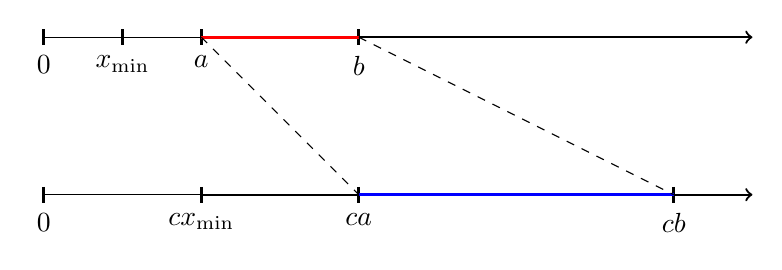
\begin{tikzpicture}
			% Draw number lines
			\draw[-] (0,2) -- (2,2);
			\draw[-] (0,0) -- (2,0);
			\draw[->,thick] (2,2) -- (9,2);
			\draw[->,thick] (2,0) -- (9,0);
			% Mark x and cx
			\draw[very thick] (1,2.1) -- (1,1.9) node[below] {$x_{\min}$};
			\draw[very thick] (2,0.1) -- (2,-0.1) node[below] {$cx_{\min}$};
			\draw[very thick] (0,2.1) -- (0,1.9) node[below] {$0$};
			\draw[very thick] (0,0.1) -- (0,-0.1) node[below] {$0$};
			\draw[very thick] (2,2.1) -- (2,1.9) node[below] {$a$};
			\draw[very thick] (4,0.1) -- (4,-0.1) node[below] {$ca$};
			\draw[very thick] (4,2.1) -- (4,1.9) node[below] {$b$};
			\draw[very thick] (8,0.1) -- (8,-0.1) node[below] {$cb$};
			% Interval on top line
			\draw[very thick,red] (2,2) -- (4,2);
			% Corresponding interval on bottom line
			\draw[very thick,blue] (4,0) -- (8,0);
			% Dashed lines mapping intervals
			\draw[dashed] (2,2) -- (4,0);
			\draw[dashed] (4,2) -- (8,0);
		\end{tikzpicture}
	\end{center}
	
	$^*$ Time permitting we can show this formally.
\end{frame}

\begin{frame}
	\frametitle{Power laws}
	
	\color{gray}
	\[
	P(X>cx)=k\,P(X>x)\quad\bigstar
	\]
	\color{black}
	
	Consider
	\[
	P(X>x)=C x^{-\alpha},
	\quad\text{i.e.}\quad
	P(X\leq x)=1-Cx^{-\alpha}.
	\]
	
	Substituting into $\bigstar$ gives
	\begin{eqnarray*}
		C (cx)^{-\alpha}
		&=& k\,C x^{-\alpha},\\[4pt]
		\Rightarrow c^{-\alpha}
		&=& k,\\[4pt]
		\Rightarrow -\alpha\log c
		&=& \log k,\\[4pt]
		\Rightarrow \alpha
		&=& -\dfrac{\log k}{\log c}.
	\end{eqnarray*}
	
	So $P(X>x)=C x^{-\alpha}$ is a solution. This gives
	\[
	f_X(x)=\frac{\mathrm{d}}{\mathrm{d}x}\big(1-Cx^{-\alpha}\big)
	=\alpha C x^{-\alpha-1}
	=A x^{-(\alpha+1)}.
	\]
	
	Observe: no value of $c>0$ can take us to $x=0$.
\end{frame}

\begin{frame}
	\frametitle{Power laws}
	
	{\bf\underline{Definition}} \par
	The {\bf Pareto distribution} has parameters $\alpha>0$ and $x_{\min}>0$ such that
	\[
	f_X(x):=
	\begin{cases}
		\dfrac{\alpha x_{\min}^{\alpha}}{x^{\alpha+1}}, & x\geq x_{\min},\\[6pt]
		0, & \text{otherwise.}
	\end{cases}
	\]
	
	A Pareto distribution is a continuous, exact power law. \par
	In general, the term ``power law'' often applies to the tail as $x\to\infty$.
	
	{\bf\underline{Mean}}
	\[
	E[X]=\frac{\alpha x_{\min}}{\alpha-1},\quad \alpha>1.
	\]
	
	{\bf\underline{Variance}}
	\[
	Var(X)=\frac{\alpha x_{\min}^2}{(\alpha-1)^2(\alpha-2)},\quad \alpha>2.
	\]
	
	Exercise: derive these expressions. \par
	{\small\color{NavyBlue} Note: $\alpha$ also appears in the normalisation constant in the PDF.}
\end{frame}

\begin{frame}
	\frametitle{Power laws}
	
	\begin{columns}
		\column[b]{0.5\textwidth}
		\begin{center}
			\fbox{\includegraphics[width=\textwidth]{powerlawdiscrete.png}}\\[3pt]
			Discrete power law ($x\geq 1$)
		\end{center}
		
		\column[b]{0.5\textwidth}
		\begin{center}
			\fbox{\includegraphics[width=\textwidth]{powerlawcont.png}}\\[3pt]
			Pareto distribution (example)
		\end{center}
	\end{columns}
\end{frame}

\begin{frame}
	\frametitle{Power laws}
	
	{\bf\underline{Definition}} \par
	\[
	p_X(k)\propto k^{-\gamma},\quad \gamma>1,\ k=1,2,\dots
	\]
	or
	\[
	f_Y(y)\propto y^{-\alpha},\quad \alpha>1,\ y\geq x_{\min}.
	\]
	
	{\small\color{NavyBlue}
		- the random variable is now the base of an exponent, not the power as in $Exp(\lambda)$.
	}\par
	
	Key observations:
	\begin{itemize}
		\item multiplying $x$ by a constant $a>1$ decreases $f_X(x)$ by a factor of $a^{\alpha+1}$;
		\item if $f_Y(y)=Ay^{-(\alpha+1)}$ then
		\[
		\log f_Y(y)=\log A-(\alpha+1)\log y;
		\]
		- log both axes and you get a straight line!
	\end{itemize}
\end{frame}

\begin{frame}
	\frametitle{Power laws}
	
	\color{gray}
	{\bf\underline{Definition}}
	\[
	p_X(k)\propto k^{-\gamma},\quad \gamma>1
	\quad\text{or}\quad
	f_Y(y)\propto y^{-\alpha},\quad \alpha>1.
	\]
	\color{black}
	
	{\bf\underline{Questions}}
	\begin{itemize}
		\item Why do we need to specify $\gamma,\alpha>1$?
		\item What are the domain constraints in the discrete / continuous case?
		\item Exponential distributions and power laws can look similar by eye. \par
		- how are they different in the tails?
	\end{itemize}
\end{frame}

\begin{frame}
	\frametitle{Power laws}
	
	{\bf\underline{Examples}} \par
	Magnitude / number of:
	\begin{itemize}
		\item income;
		\item solar flares;
		\item volcanic activity;
		\item academic citations.
	\end{itemize}
	
	{\small\color{NavyBlue}
		- power laws typically describe the frequency of an ``amount of stuff''.
	}
\end{frame}

\begin{frame}
	\frametitle{Example 6D}
	
	Two models are proposed for the size $X$ (in GB) of large data files
	stored on a server.
	
	\begin{itemize}
		\item Model A (exponential tail): $X_A \sim Exp(\lambda)$ with $\lambda=1$.
		\item Model B (heavy tail): $X_B \sim \text{Pareto}(\alpha, x_{\min})$
		with $\alpha = 2$ and $x_{\min}=1$:
		\[
		f_{X_B}(x) =
		\begin{cases}
			\dfrac{2\cdot 1^2}{x^{3}}, & x \ge 1,\\[4pt]
			0, & x < 1.
		\end{cases}
		\]
	\end{itemize}
	
	\begin{enumerate}[(a)]
		\item Compute $P(X_A > 5)$ and $P(X_B > 5)$.
		\item Compute (or recall) the means $E[X_A]$ and $E[X_B]$.
		\item Which model assigns a higher probability to very large files
		(e.g.\ size $> 10$)? Explain briefly using the form of the tail
		probabilities.
		\item On a log-scale:
		\begin{itemize}
			\item What does $\log f_{X_A}(x)$ look like as a function of $x$?
			\item What does $\log f_{X_B}(x)$ look like as a function of $\log x$?
		\end{itemize}
		How could you use plots to distinguish exponential vs power-law tails
		in data?
	\end{enumerate}
\end{frame}

\begin{frame}
	\frametitle{Example 6D (answer)}
	
	\textbf{(a)} Exponential:
	\[
	P(X_A>5) = e^{-\lambda\cdot 5} = e^{-5}.
	\]
	Pareto:
	\[
	P(X_B>5) = \int_5^\infty \frac{2}{x^3}\,dx
	= \left[-\frac{1}{x^2}\right]_{5}^{\infty}
	= \frac{1}{25}.
	\]
	\textbf{(b)}
	\[
	E[X_A] = \frac{1}{\lambda} = 1.
	\]
	For Pareto with $\alpha=2, x_{\min}=1$:
	\[
	E[X_B] = \frac{\alpha x_{\min}}{\alpha-1}
	= \frac{2\cdot 1}{2-1} = 2.
	\]
	
\end{frame}

\begin{frame}
	\frametitle{Example 6D (answer)}
	\textbf{(c)} For large $x$,
	\[
	P(X_A > x) = e^{-x} \quad(\text{decays exponentially}),
	\]
	whereas
	\[
	P(X_B > x) \propto x^{-2} \quad(\text{polynomial decay}).
	\]
	So $X_B$ assigns much higher probability to very large values:
	a \emph{heavier tail}.
	\textbf{(d)} Exponential:
	\[
	\log f_{X_A}(x) = \log \lambda - \lambda x
	\]
	is a straight line if we plot $\log f$ vs $x$ (semilog plot). \\
	Pareto:
	\[
	f_{X_B}(x) = 2x^{-3}
	\Rightarrow \log f_{X_B}(x) = \log 2 - 3\log x,
	\]
	which is a straight line when we plot $\log f$ vs $\log x$
	(log–log plot). \\
	So:
	\begin{itemize}
		\item exponential tails look linear on a semilog plot;
		\item power-law tails look linear on a log–log plot.
	\end{itemize}
\end{frame}


% ============================================================
% Week 7
% ============================================================

\section{Week 7: sampling theory}
%Limit laws

\begin{frame}
	\frametitle{Sampling}
	Say you know $P(1<X<2)=0.9999$. \par
	Let $x$ be a realised value of $X$. \par
	Formally, $x$ is {\bf sampled} (or simulated) from the distribution of $X$. \par
	What can you say about $x$? \par
	\vspace{10pt}
	Aside: random number generators typically produce samples from $U(0,1)$. \par
	{\small\color{NavyBlue}
		How can we use this to sample from any known CDF $F_X$? \\
		(Hint: $x = F_X^{-1}(u)$ where $u\sim U(0,1)$.)
	}
\end{frame}

\begin{frame}
	\frametitle{What is probability? (recap)}
	{\bf\underline{Frequentist interpretation}} \par
	Probability is the long-run relative frequency of an event occurring when an experiment is repeated under identical conditions:
	\[
	P(A)=\lim_{n\rightarrow\infty}\frac{k_n(A)}{n}
	\]
	where $k_n(A)$ is the observed number of occurrences of $A$ in $n$ trials. \par
	{\small\color{NavyBlue}
		This is objective and based on observed data: each event has a true, fixed parameter defining its probability. \\
		The remainder of MATH163 will assume the frequentist interpretation of probability.
	} \par
	{\bf\underline{Bayesian interpretation}} \par
	Probability represents a degree of belief or certainty about an event, updated as new evidence is observed. Recall:
	\[
	P(\theta\vert D)=\frac{P(D\vert\theta)P(\theta)}{P(D)},
	\]
	where $P(\theta\vert D)$ is the updated probability of a parameter $\theta$ given data $D$. \par
	{\small\color{NavyBlue}
		You will still need to understand and use Bayes' rule in MATH163!
	}
\end{frame}

\begin{frame}
	\frametitle{Samples}
	{\bf\underline{Definitions}}
	\begin{itemize}
		\item {\bf i.i.d.} means ``independent and identically distributed''.
		\item If $X_1,X_2,\dots,X_n$ are i.i.d.\ then $\{X_1,X_2,\dots,X_n\}$ is a {\bf random sample} from this distribution.\\
		{\small\color{NavyBlue}
			e.g.\ $X_i$ are successive rolls of a fair die.
		}
		\item After observation ($X_1=x_1,\dots,X_n=x_n$), the sequence $x_1,\dots,x_n$ is the {\bf sample data}.
		\item In practice, the term {\bf sample} is used for both the random variables and the observed data.
		\item $\bar X_n:=\frac{1}{n}\sum_{i=1}^n X_i$ is the {\bf sample mean} of a sample of size $n$.\\
		{\bf The subscript $n$ always denotes the sample size.}
	\end{itemize}
	Note: sampling without replacement means successive observations are not independent.
\end{frame}

\begin{frame}
	\frametitle{Sampling distributions}
	\begin{itemize}
		\item Collect a sample from a population (sample size $n$).
		\item Calculate the sample mean.
		\item Repeat this process (with replacement), collecting a set of sample means.
		\item These sample means will (usually) not be equal — they follow a distribution.
		\item This distribution is the {\bf sampling distribution of the mean}.
		\item Caveat: you need a big enough sample and a big enough population for this distribution to be interesting — why?
	\end{itemize}
	
	\begin{center}
		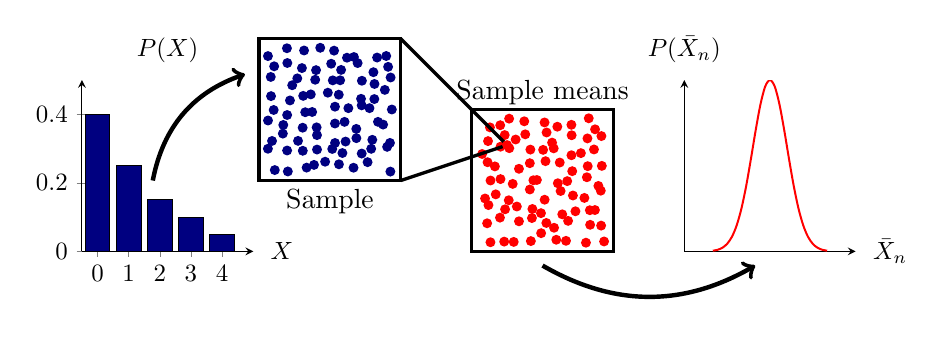
\begin{tikzpicture}[scale=0.9]
			% (a) Original X distribution (e.g. geometric)
			\begin{scope}[shift={(0,0)}]
				\begin{axis}[
					at={(0,0)},
					anchor=south west,
					width=4cm, height=4cm,
					ybar,
					axis x line=middle,
					axis y line=left,
					xlabel style={at={(rel axis cs:1.05,0)}, anchor=west},
					ylabel style={at={(rel axis cs:.5,1.05)}, anchor=south, rotate=-90},
					xmin=-.5, xmax=5,
					ymin=0, ymax=0.5,
					xlabel={$X$}, ylabel={$P(X)$},
					xtick={0,1,2,3,4},
					]
					\addplot[fill=NavyBlue] coordinates {(0,0.4) (1,0.25) (2,0.15) (3,0.1) (4,0.05)};
				\end{axis}
			\end{scope}
			
			% (b) Sample scatter
			\draw[very thick] (2.5,1) rectangle (4.5,3)
			node[midway, below, yshift=-25pt] {Sample};
			\foreach \x in {2.7,2.9,...,4.3} {
				\foreach \y in {1.2,1.4,...,2.8} {
					\fill[NavyBlue] (\x+rand*0.08,\y+rand*0.08) circle (2pt);
				}
			}
			
			% (c) Sample means cloud
			\draw[very thick] (5.5,0) rectangle (7.5,2)
			node[midway, below, yshift=40pt] {Sample means};
			\foreach \x in {5.7,5.9,...,7.3} {
				\foreach \y in {.2,.4,...,1.8} {
					\fill[red] (\x+rand*0.08,\y+rand*0.08) circle (2pt);
				}
			}
			\draw[very thick, black] (4.5,1) -- (6,1.5);
			\draw[very thick, black] (4.5,3) -- (6,1.5);
			\fill[red] (6,1.5) circle (2pt);
			
			\draw[ultra thick, black, ->, bend left] (1,1) to (2.3,2.5);
			\draw[ultra thick, black, ->, bend right] (6.5,-.2) to (9.5,-.2);
			
			% (d) Approximate normal for sample mean
			\begin{scope}[shift={(8.5,0)}]
				\begin{axis}[
					anchor=south west,
					width=4cm, height=4cm,
					axis lines=middle,
					xlabel style={at={(axis description cs:1.05,0)}, anchor=west},
					ylabel style={at={(axis description cs:0,1.05)}, anchor=south},
					xlabel={$\bar X_n$}, ylabel={$P(\bar X_n)$},
					xmin=1.5, xmax=4.5,
					ymin=0, ymax=1,
					xtick=\empty, ytick=\empty,
					domain=2:4
					]
					\addplot[smooth,red,thick] {exp(-((x-3)^2)/(2*0.3^2))};
				\end{axis}
			\end{scope}
		\end{tikzpicture}
	\end{center}
\end{frame}

\begin{frame}
	\frametitle{Sampling distributions: mean}
	{\bf Key idea: we can view the mean of a sample of size $n$ as a random variable.} \par
	$\bar X_n$ denotes a random variable that follows the sampling distribution of the mean of $X$.
	\begin{itemize}
		\item $n$ is the sample size.
		\item $\mu$ is the population mean.
		\item $\sigma^2$ is the population variance.
	\end{itemize}
	{\bf\underline{Mean}}
	\begin{eqnarray*}
		E[\bar X_n]
		&=&E\left[\frac{1}{n}\sum_{i=1}^n X_i\right]\\
		&=&\frac{1}{n}\sum_{i=1}^n E[X_i] \quad\text{(linearity of expectation)}\\
		&=&\frac{1}{n}\times nE[X_1] \quad\text{(i.i.d.)}\\
		&=&E[X_1]=\mu.
	\end{eqnarray*}
	So the mean of the sampling distribution of the mean is equal to the population mean.
\end{frame}

\begin{frame}
	\frametitle{Standard error}
	What is the variance of the sampling distribution of the mean?
	\begin{eqnarray*}
		Var(\bar X_n)
		&=&Var\left(\frac{1}{n}\sum_{i=1}^n X_i\right)\\
		&=&\frac{1}{n^2}\sum_{i=1}^nVar(X_i)
		\quad\text{(independence)}\\
		&=&\frac{1}{n^2}n\sigma^2=\frac{\sigma^2}{n}.
	\end{eqnarray*}
	The {\bf standard error} of the mean is the standard deviation of the sampling distribution of the mean:
	\[
	\sigma_{\bar X}=\frac{\sigma}{\sqrt{n}}.
	\]
\end{frame}

\begin{frame}
	\frametitle{The laws of large numbers}
	There are 2 laws of large numbers, but they both intuitively say: \par
	{\bf As sample size gets larger, the mean of the sample converges to the mean of the population.} \par
	Formally, if $X_1,X_2,\dots,X_n$ are i.i.d.\ with mean $\mu$ and variance $\sigma^2$, then
	\[
	\bar X_n \xrightarrow{n\rightarrow\infty} \mu.
	\]
\end{frame}

\begin{frame}
	\frametitle{The laws of large numbers}
	Let $X_1,X_2,\dots,X_n$ be i.i.d.\ with $E(X_i)=\mu$. \par
	{\bf\underline{The weak law of large numbers} (WLLN):} \par
	\[
	\lim_{n\rightarrow\infty} P\left(\vert\bar X_n-\mu\vert<\epsilon\right)=1
	\quad\text{or equivalently}\quad
	\lim_{n\rightarrow\infty}P\left(\vert\bar X_n-\mu\vert\geq\epsilon\right)=0.
	\]
	{\bf\underline{Lemma (Chebyshev's inequality)}} \par
	If $X$ is any random variable with $E[X^2]<\infty$, then for any $\epsilon >0$ we have:
	\[
	P(|X|\geq\epsilon)\leq\frac{E[X^2]}{\epsilon^2}.
	\]
	{\bf\underline{Proof of lemma}} \par
	Define the {\bf indicator function}
	\[
	\mathbf 1_{|X|\geq\epsilon} =
	\begin{cases}
		1, & |X|\geq\epsilon,\\
		0, & |X|<\epsilon.
	\end{cases}
	\]
	Then
	\[
	E[X^2]\ \ge E\big[X^2\mathbf 1_{|X|\geq\epsilon}\big]
	\ \ge E\big[\epsilon^2\mathbf 1_{|X|\geq\epsilon}\big]
	=\epsilon^2P(|X|\geq\epsilon)\quad\blacksquare
	\]
\end{frame}

\begin{frame}
	\frametitle{The laws of large numbers}
	{\bf\underline{Proof of WLLN}} \par
	Apply Chebyshev's inequality to $X=\bar X_n-\mu$:
	\begin{eqnarray*}
		E[(\bar X_n-\mu)^2]
		&=&Var(\bar X_n)
		=\frac{\sigma^2}{n},\\
		P\left(\vert\bar X_n-\mu\vert\geq\epsilon\right)
		&\leq&\frac{E[(\bar X_n-\mu)^2]}{\epsilon^2}
		=\frac{\sigma^2}{n\epsilon^2}
		\xrightarrow{n\rightarrow\infty}0\quad\blacksquare
	\end{eqnarray*}
	{\small\color{NavyBlue}
		Note the limit is $n\rightarrow\infty$, not $\epsilon\rightarrow 0$.
	}
\end{frame}

\begin{frame}
	\frametitle{The laws of large numbers}
	Recall $\bar X_n$ is the mean of $n$ i.i.d.\ random variables with $E[X_i]=\mu$. \par
	{\bf\underline{Weak law of large numbers (WLLN):}}
	\[
	\bar X_n\xrightarrow{p}\mu\ \text{as }n\rightarrow\infty,
	\quad\text{i.e.}\quad
	\lim_{n\rightarrow\infty}P\left(|\bar X_n-\mu|<\epsilon\right)=1.
	\]
	{\small\color{NavyBlue}
		``Convergence in probability'': a sequence of probabilities converges to 0.
	} \par
	{\bf\underline{Strong law of large numbers (SLLN):}} \par
	Under slightly stronger conditions,
	\[
	\bar X_n\xrightarrow{a.s.}\mu\ \text{as }n\rightarrow\infty,
	\quad\text{i.e.}\quad
	P\left(\lim_{n\rightarrow\infty}\bar X_n=\mu\right)=1.
	\]
	{\small\color{NavyBlue}
		``Almost sure convergence'': with probability 1, the sequence converges to $\mu$. \\
		Even as we approach this limit, there is still variation in sample means for finite $n$.
	}
\end{frame}

\begin{frame}
	\frametitle{Approximate PMF}
	Let $X_1,X_2,\dots,X_n$ be i.i.d.\ with $p_X(k)=P(X_1=k)>0$. Then: \par
	{\bf\underline{Corollary of WLLN}} \par
	\[
	\frac{1}{n}\sum_{i=1}^n\mathbf 1_{X_i=k}
	\xrightarrow{n\rightarrow\infty} E[\mathbf 1_{X_1=k}]
	=p_X(k).
	\]
	{\small\color{NavyBlue}
		As samples get larger, relative frequency converges to probability mass.
	} \par
	More precisely, for all $\epsilon>0$ and $n=1,2,\dots$,
	\[
	P\left(\left|\frac{1}{n}\sum_{i=1}^n\mathbf 1_{X_i=k}-p_X(k)\right|\geq\epsilon\right)
	\leq\frac{1}{4n\epsilon^2}\xrightarrow{n\rightarrow\infty}0.
	\]
	{\bf\underline{Proof}} \par
	\[
	P\left(\left|\frac{1}{n}\sum_{i=1}^n\mathbf 1_{X_i=k}-p_X(k)\right|\geq\epsilon\right)
	\leq\frac{Var(\mathbf 1_{X_1=k})}{n\epsilon^2}
	=\frac{p_X(k)(1-p_X(k))}{n\epsilon^2}
	\leq\frac{1}{4n\epsilon^2},
	\]
	using that $\mathbf 1_{X_i=k}\sim \mathrm{Bernoulli}(p_X(k))$ and $\sup_{0\leq a\leq 1}a(1-a)=\frac14$.
\end{frame}

\begin{frame}
	\frametitle{Approximate CDF}
	The same idea applies to CDFs (written out for completeness). \par
	Let $X_1,X_2,\dots,X_n$ be i.i.d.\ with $F_X(t)=P(X_1\leq t)$. Then: \par
	{\bf\underline{Corollary of WLLN}} \par
	\[
	\frac{1}{n}\sum_{i=1}^n\mathbf 1_{X_i\leq t}
	\xrightarrow{n\rightarrow\infty}E[\mathbf 1_{X_1\leq t}]
	=F_X(t).
	\]
	More precisely, for all $\epsilon>0$ and $n=1,2,\dots$,
	\[
	P\left(\left|\frac{1}{n}\sum_{i=1}^n\mathbf 1_{X_i\leq t}-F_X(t)\right|\geq\epsilon\right)
	\leq\frac{1}{4n\epsilon^2}\xrightarrow{n\rightarrow\infty}0.
	\]
	{\bf\underline{Proof}} \par
	\[
	P\left(\left|\frac{1}{n}\sum_{i=1}^n\mathbf 1_{X_i\leq t}-F_X(t)\right|\geq\epsilon\right)
	\leq\frac{Var(\mathbf 1_{X_1\leq t})}{n\epsilon^2}
	=\frac{F_X(t)(1-F_X(t))}{n\epsilon^2}
	\leq\frac{1}{4n\epsilon^2}.
	\]
	Recall the frequentist interpretation of statistics!
\end{frame}

\begin{frame}
	\frametitle{Example 7A}
	Let $X_1, X_2, \dots, X_n$ be independent random variables with $X_i \sim \text{Geom}(p)$ for all $i$, i.e.
	\[
	P(X_i = k) = (1 - p)^k p, \quad k = 0,1,2,\dots
	\]
	Let $\bar{X}_n = \frac{1}{n} \sum_{i=1}^{n} X_i$ be the sample mean. Using the WLLN/Chebyshev inequality, determine how large $n$ must be so that
	\[
	P(|\bar{X}_n - \mathbb{E}[X]| \geq 0.1) \leq 0.01.
	\]
	
	\begin{center}
		\fbox{\includegraphics[width=.2\textwidth]{countdown.jpg}}
	\end{center}
\end{frame}

\begin{frame}
	\frametitle{The central limit theorem (CLT)}
	{\bf CLT:} if sample size $n$ is fixed across all samples and $\sigma^2<\infty$, then the sampling distribution of the mean is approximately normal for large $n$.
	\begin{itemize}
		\item Formally,
		\begin{eqnarray*}
			\bar X_n &\xrightarrow{d}& N\!\left(\mu, \frac{\sigma^2}{n}\right)\quad\text{as }n\rightarrow\infty,\\
			\text{or}\quad
			\frac{\bar X_n-\mu}{\sigma/\sqrt{n}}
			&\xrightarrow{d}& N(0,1)\quad\text{as }n\rightarrow\infty,
		\end{eqnarray*}
		where $\mu$ is the mean and $\sigma$ the s.d.\ of $X$.
		\item Is this surprising? Is it obvious?
		\item This is the classical CLT; there are generalised variants. \\
		{\small\color{NavyBlue}
			We can account for sampling from non-identical distributions, or even certain heavy-tailed cases (with care).
		}
	\end{itemize}
\end{frame}

\begin{frame}
	\frametitle{The central limit theorem (CLT)}
	\centering
	\fbox{\includegraphics[width=.5\textwidth]{clt.jpg}}
\end{frame}

\begin{frame}
	\frametitle{Example 7B}
	For a fair coin ($p = 0.5$), let $X_1, X_2, \dots, X_n$ be i.i.d.\ geometric random variables, where $X_i$ represents the number of failures before the first success. Set $n = 100$. Use the CLT to approximate:
	\[
	P\left( \bar{X}_n \geq \mathbb{E}[X] + 0.1 \right).
	\]
	
	\begin{center}
		\fbox{\includegraphics[width=.2\textwidth]{countdown.jpg}}
	\end{center}
\end{frame}

\begin{frame}
	\frametitle{The central limit theorem (CLT)}
	Why are so many variables (approximately) normally distributed? \par 
	Let $X_1, X_2, \dots, X_n$ be independent random variables with means $\mu_i$ and variances $\sigma_i^2$. Consider the normalised sum:
	\[
	S_n = \frac{1}{\sqrt{\sum_{i=1}^{n} \sigma_i^2}}
	\left( \sum_{i=1}^{n} (X_i - \mu_i) \right).
	\]
	Then the {\bf generalised central limit theorem (GCLT)} states:
	\[
	S_n\xrightarrow{d}N(0,1)
	\]
	assuming the {\bf Lindeberg condition} is satisfied. \par
	The Lindeberg condition ensures that no individual variable has too large an impact on the sum. Formally, for each $\epsilon > 0$, it requires:
	\[
	\frac{1}{\sum_{i=1}^{n} \sigma_i^2}
	\sum_{i=1}^{n}
	E\Big[ (X_i - \mu_i)^2 \mathbf{1}_{|X_i - \mu_i| > \epsilon} \Big]
	\to 0 \quad \text{as } n \to \infty.
	\]
\end{frame}

\begin{frame}
	\frametitle{The central limit theorem (CLT)}
	Which of the following variables do you expect are {\bf not} normally distributed? Why?
	\begin{itemize}
		\item Human height
		\item Income in the UK
		\item IQ
		\item Exam scores in a large class
		\item Time to failure of electronic devices
		\item Blood pressure
		\item Daily temperature in a city
		\item Shoe size in adult women
	\end{itemize}
\end{frame}

\begin{frame}
	\frametitle{Example 7C}
	Recall the Bernoulli distribution with $P(X=1)=p$, $P(X=0)=1-p$. \par
	Let $X_1,\dots,X_n$ be i.i.d.\ Bernoulli$(p)$. The sample mean is
	\[
	\bar X_n=\frac{1}{n}\sum_{i=1}^n X_i.
	\]
	Consider the {\it sum} of $n$ Bernoulli trials:
	\[
	S_n=\sum_{i=1}^n X_i.
	\]
	We have
	\[
	P(S_n=k)={n\choose k} p^k(1-p)^{n-k},
	\]
	which is binomial. By the CLT,
	\[
	S_n\xrightarrow{d} N\big(np,\;np(1-p)\big)\quad\text{as }n\rightarrow\infty.
	\]
	{\small\color{NavyBlue}
		So for large $n$, the normal distribution can approximate the binomial distribution (especially when $p$ is not too close to 0 or 1).
	}
	
	\begin{center}
		\fbox{\includegraphics[width=.2\textwidth]{countdown.jpg}}
	\end{center}
\end{frame}

\begin{frame}
	\frametitle{Example 7C (answer)}
	
	\textbf{(a) Mean and variance}
	For $X \sim \mathrm{Bin}(n,p)$:
	\[
	E[X] = np, \qquad Var(X) = np(1-p).
	\]
	With $n=100$, $p=0.3$:
	\[
	E[X] = 100 \cdot 0.3 = 30, \qquad
	Var(X) = 100 \cdot 0.3 \cdot 0.7 = 21.
	\]
	So $\sigma = \sqrt{21} \approx 4.58$.
	
	\vspace{6pt}
	\textbf{(b) Normal approximation with continuity correction}
	\[
	X \approx N(\mu,\sigma^2) = N(30,21).
	\]
	Using a continuity correction:
	\[
	P(25 \le X \le 35)
	\approx P(24.5 < X < 35.5).
	\]
	Standardise:
	\[
	Z = \frac{X - \mu}{\sigma}, \quad Z \sim N(0,1).
	\]
	Then
	\[
	P(24.5 < X < 35.5)
	= P\!\left(\frac{24.5-30}{4.58} < Z < \frac{35.5-30}{4.58}\right).
	\]
	Numerically:
	\[
	\frac{24.5-30}{4.58} \approx -1.20,
	\qquad
	\frac{35.5-30}{4.58} \approx 1.20.
	\]
	So
	\[
	P(25 \le X \le 35)
	\approx P(-1.20 < Z < 1.20)
	= \Phi(1.20) - \Phi(-1.20)
	\approx 0.884 - 0.116
	\approx 0.768.
	\]
	
	\vspace{4pt}
	\textbf{(c) Comment}
	\begin{itemize}
		\item Exact binomial calculation in R:
		{\small \texttt{pbinom(35,100,0.3) - pbinom(24,100,0.3)}}.
		\item The exact value is close to $0.77$, so the normal approximation
		(with continuity correction) is very reasonable here.
	\end{itemize}
	
\end{frame}

\begin{frame}
	\frametitle{Example 7D: normal approximation to a binomial}
	
	Suppose $X \sim \mathrm{Bin}(n,p)$ with $n=100$ and $p=0.3$.
	Here $X$ is the number of successes in $100$ independent trials.
	
	We are interested in
	\[
	P(25 \le X \le 35).
	\]

	\begin{enumerate}[(a)]
		\item Write down the mean and variance of $X$.
		\item Use a normal approximation to estimate $P(25 \le X \le 35)$, including
		a continuity correction.
		\[
		X \approx N(np,\,np(1-p)).
		\]
		\item (Optional) Use R or a calculator to compute the exact binomial
		probability and compare it with your normal approximation.
		Is the approximation reasonable?
	\end{enumerate}
	
	\begin{center}
		\fbox{\includegraphics[width=.2\textwidth]{countdown.jpg}}
	\end{center}
	
\end{frame}

%----------------------------------------
% Estimators
%----------------------------------------

\begin{frame}
	\frametitle{Estimators}
	{\bf\underline{Definitions}} \par
	\begin{itemize}
		\item A {\bf statistic} is any function of a random sample $X_1,X_2,\dots,X_n$.
		\item A {\bf parameter} $\theta$ is a property of the population the sample is drawn from.
		\item An {\bf estimator} $\hat\theta$ is a function of the sample used to estimate $\theta$.
	\end{itemize}
	Example: we typically estimate the population mean $\mu$ with the sample mean $\bar X_n$. \par
	{\small\color{NavyBlue}
		This seems obvious, but from the CLT we know $\bar X_n$ has non-zero variance, so there is uncertainty in the estimate.
	} \par
	What about estimating variance? \par
	A ``naïve'' estimator using the (unknown) population mean:
	\[
	S_0^2:=\frac{1}{n}\sum_{i=1}^n(X_i-\mu)^2.
	\]
	In practice, we do not know $\mu$, so we replace it with $\bar X_n$:
	\[
	S_0^2:=\frac{1}{n}\sum_{i=1}^n(X_i-\bar X_n)^2.
	\]
\end{frame}

\begin{frame}
	\frametitle{Estimators}
	Recall: $E[aX]=aE[X]$ and, if $X$ and $Y$ are independent, $E[XY]=E[X]E[Y]$. \par
	Also, $\sigma^2=E[X^2]-\mu^2\Rightarrow E[X^2]=\sigma^2+\mu^2$. \par
	{\tiny
		\begin{eqnarray*}
			E[S_0^2]
			&=&E\left[\frac{1}{n}\sum_{i=1}^n\left(X_i-\frac{1}{n}\sum_{j=1}^nX_j\right)^2\right] \\
			&=&\sum_{i=1}^n\frac{1}{n}E\left[X_i^2-\frac{2}{n}X_i\sum_{j=1}^nX_j+\frac{1}{n^2}\sum_{j=1}^nX_j\sum_{k=1}^nX_k\right] \\
			&=&\frac{1}{n}\sum_{i=1}^n\left(E[X_i^2]-\frac{2}{n}\left(\sum_{j\neq i}E[X_iX_j]+E[X_i^2]\right)+\frac{1}{n^2}\sum_j\sum_{k\neq j}E[X_jX_k]+\frac{1}{n^2}\sum_jE[X_j^2]\right) \\
			&=&\frac{1}{n}\sum_{i=1}^n\left(\frac{n-1}{n}E[X_i^2]-\frac{2}{n}\sum_{j\neq i}E[X_iX_j]+\frac{1}{n^2}\sum_j\sum_{k\neq j}E[X_jX_k\right) \\
			&=&\frac{1}{n}\sum_{i=1}^n\left(\frac{n-1}{n}(\sigma^2+\mu^2)-\frac{2}{n}(n-1)\mu^2+\frac{1}{n^2}n(n-1)\mu^2\right) \\
			&=&\frac{1}{n}\sum_{i=1}^n\frac{n-1}{n}\sigma^2 \\
			&=&\frac{n-1}{n}\sigma^2.
		\end{eqnarray*}
	}
	So $S_0^2$ will always {\bf under-estimate} $\sigma^2$ on average — it is a {\bf biased} estimator. Why is that?
\end{frame}

\begin{frame}
	\frametitle{Estimators}
	Recall: $S_0^2:=\frac{1}{n}\sum_{i=1}^n(X_i-\bar X_n)^2$ and $E[S_0^2]=\frac{n-1}{n}\sigma^2$. \par
	This is an example of a {\bf biased estimator}. \par
	{\bf\underline{Definitions}} \par
	Let $\hat\theta$ be an estimator of a parameter $\theta$. Then:
	\begin{itemize}
		\item $\hat\theta$ is {\bf unbiased} if $E[\hat\theta]=\theta$.
		\item $\hat\theta$ is {\bf consistent} if
		\[
		\lim_{n\rightarrow\infty}P(|\hat\theta-\theta|\geq\epsilon)=0
		\quad\forall\epsilon>0.
		\]
	\end{itemize}
	{\bf Consistency is about what happens if we could sample forever. Bias is about the fact we can’t.} \par
	The sample mean $\bar X_n$ is an unbiased, consistent estimator of $\mu$. \par
	The quantity $S_0^2$ is a biased but consistent estimator of $\sigma^2$. \par
	Can you construct an unbiased estimator of $\sigma^2$?
\end{frame}

\begin{frame}
	\frametitle{Estimators}
	{\bf\underline{Definition}} \par
	The usual {\bf sample variance} is
	\[
	S^2:=\frac{1}{n-1}\sum_{i=1}^n(X_i-\bar X_n)^2.
	\]
	Then $E[S^2]=\sigma^2$, so $S^2$ is an {\bf unbiased} estimator of the population variance.
	% (Cochran's theorem gives a chi-squared distribution with n-1 d.o.f. when X is normal.)
\end{frame}

\begin{frame}
	\frametitle{Example 7E: Capture-mark-recapture}
	Recall the capture-mark-recapture set-up:
	\begin{itemize}
		\item Closed population of unknown size $N$
		\item First sample: capture and mark $K$ individuals, then release
		\item Second sample: capture $n$ individuals
		\item Let $k$ be the number of marked individuals in the second sample
		\item $k\sim NB(K,N-K,n)$, $E[k]=\frac{Kn}{N}$
	\end{itemize}
	{\small\color{NavyBlue} Note the abse of notation: lower case letters for random variables} \par
	Intuitive estimator of $N$:
	$$\hat N := \frac{Kn}{k}$$
	{\bf\underline{Question}} \par
	Is $\hat N$ unbiased?
\end{frame}

\begin{frame}
	\frametitle{Example 7E (answer)}
	Treat $\hat N$ as a random variable (hypergeometric):
	\begin{itemize}
		\item $E[\hat N] = \dfrac{Kn}{k}$
		\item $\hat k = Kn \,\dfrac{1}{N}$, so $E[\hat k] = Kn\,E\left[\dfrac{1}{\hat N}\right]$
		\item For positive random variables, recall:
		$$E\left[\frac{1}{X}\right] > \frac{1}{E[X]}$$
		\item Hence (ignoring the rare case $X=0$):
		$$E[\hat N] = Kn\,E\left[\frac{1}{k}\right] > Kn\,\frac{1}{E[k]}
		= n_1 n_2\,\frac{k}{n_1 n_2} = k$$
	\end{itemize}
	So $\hat N$ is a {\bf biased} estimator of $N$: on average it {\bf overestimates} the true population size.
\end{frame}

\begin{frame}
	\frametitle{Notation}
	From now on, let $X_1,X_2,\dots,X_n$ be i.i.d.\ random variables: a sample (with replacement) of size $n$. \par
	{\small\color{NavyBlue}
		Each $X_i$ corresponds to a single measurement of something; the collection forms a sample.
		For example, each $X_i$ could be the outcome of a coin toss, a die roll, a height, a temperature, etc.
	} \par
	Then we define:
	\begin{itemize}
		\item $\mu$: population mean.
		\item $\bar X_n$: sample mean.
		\item $\sigma$: population standard deviation.
		\item $\sigma_X=S=\sqrt{\frac{1}{n-1}\sum_{i=1}^n(X_i-\bar X_n)^2}$: sample standard deviation.
		\item $\sigma_{\bar X}=\frac{\sigma}{\sqrt n}$: standard error of the mean.
		\item $\hat\sigma_{\bar X}=\frac{S}{\sqrt n}$: estimate of the standard error using the sample s.d.\\
		{\small\color{NavyBlue}
			Annoyingly this often just gets called ``the standard error'' in practice.
		}
	\end{itemize}
\end{frame}

\begin{frame}
	\frametitle{Example 7F}
	
	We toss a (possibly biased) coin $n$ times. Let $X$ be the number of Heads. \par
	The usual estimator of $p := P(\text{Heads})$ is
	\[
	\hat p = \frac{X}{n},
	\]
	which is unbiased. \par\medskip
	
	Suppose instead we use a \emph{smoothed} estimator:
	\[
	\tilde p = \frac{X+1}{n+2}.
	\]
	(You can think of this as pretending we saw 1 extra Head and 1 extra Tail.) \par\medskip
	
	\textbf{Questions}
	\begin{enumerate}[(a)]
		\item Show that $E[\tilde p] = \dfrac{np+1}{n+2}$.
		\item Is $\tilde p$ unbiased? If not, what is its bias?
		\item For which values of $p$ is the bias positive? For which is it negative?
		\item Why might someone still choose to use $\tilde p$ instead of $\hat p$ when $n$ is small?
		(Give a short, intuitive explanation.)
	\end{enumerate}
\end{frame}

\begin{frame}
	\frametitle{Example 7F (answer)}
	
	Recall $X \sim \text{Bin}(n,p)$ and $E[X] = np$. \par
	
	{\bf (a)}
	\[
	E[\tilde p]
	= E\!\left[\frac{X+1}{n+2}\right]
	= \frac{E[X] + 1}{n+2}
	= \frac{np + 1}{n+2}.
	\]
	
	{\bf (b)} $\tilde p$ is unbiased iff $E[\tilde p] = p$. Here
	\[
	\text{Bias}(\tilde p)
	= E[\tilde p] - p
	= \frac{np+1}{n+2} - p
	= \frac{1 - 2p}{n+2}.
	\]
	So it is \alert{not} unbiased unless $p=\tfrac12$. \par
	{\bf (c)} Sign of the bias:
	\[
	\text{Bias}(\tilde p) = \frac{1-2p}{n+2}
	\begin{cases}
		> 0, & p < \tfrac12,\\[4pt]
		= 0, & p = \tfrac12,\\[4pt]
		< 0, & p > \tfrac12.
	\end{cases}
	\]
	So $\tilde p$ is \emph{pulled towards $0.5$}: too big when $p<0.5$, too small when $p>0.5$.
\end{frame}

\begin{frame}
	\frametitle{Example 7F (answer)}
	{\bf (d)} Intuition:
	\begin{itemize}
		\item For small $n$, $\hat p = X/n$ can be very extreme (e.g.\ $0$ or $1$).
		\item $\tilde p$ adds ``pseudo-observations'', shrinking estimates towards $0.5$.
		\item This introduces bias but can reduce variability and give more stable estimates
		when data are scarce.
	\end{itemize}
	{\bf Key point: the estimator is only biased when the coin is biased, but the added bias in the estimator shrinks the bias of the coin.} \par
	This is the seed of Laplace/add-on smoothing:
	\begin{itemize}
		\item slightly more \alert{bias};
		\item often much lower \alert{variance} $\Rightarrow$ better overall accuracy.
		\item This idea (add-one / Laplace smoothing) is widely used:
		\begin{itemize}
			\item estimating word probabilities in language models;
			\item avoiding zero probabilities in simple classifiers.
		\end{itemize}
		\item As $n \to \infty$, $\tilde p \to p$ (it is still a \textbf{consistent} estimator).
	\end{itemize}
\end{frame}


% ============================================================
% Week 8
% ============================================================

\section{Week 8: statistical testing I}

\begin{frame}
	\frametitle{Statistical testing}
	When we collect data, we sample from a population. There are several questions we can ask about a sample or samples:
	\begin{itemize}
		\item Has my sample come from the population I think it has come from?
		\item Have these $2$ samples come from the same population or not?
		\item Can I tell from my sample if this population follows the distribution I think it follows?
	\end{itemize}
\end{frame}

\begin{frame}
	\frametitle{$z$-test}
	Testing the mean of the sample $\bar X_n$ against the hypothesised population mean $\mu_0$:
	\begin{table}[h]
		\centering
		\begin{tabular}{|c|c|c|c|}
			\hline
			\textbf{Sample Size} & \textbf{Population Normal?} & \textbf{Variance Known?} & \textbf{Test to Use} \\ 
			\hline
			\( n < 30 \) & $\checkmark$ & $\checkmark$ & \( z \)-test \\ 
			\( n < 30 \) & $\checkmark$ & $\times$      & \( t \)-test \\ 
			\( n < 30 \) & $\times$      & $\checkmark$ & Neither$^*$ \\ 
			\( n < 30 \) & $\times$      & $\times$     & Neither$^*$ \\ 
			\( n \ge 30 \) & $\checkmark$ & $\checkmark$ & \( z \)-test \\ 
			\( n \ge 30 \) & $\checkmark$ & $\times$      & \( t \)-test \\ 
			\( n \ge 30 \) & $\times$      & $\checkmark$ & \( z \)-test \\ 
			\( n \ge 30 \) & $\times$      & $\times$     & \( t \)-test \\ 
			\hline
		\end{tabular}
	\end{table}
	$^*$Use a nonparametric test (not covered in MATH163).
\end{frame}

\begin{frame}
	\frametitle{$\bigstar$ $z$-test}
	A $z$-test is performed as follows:
	\begin{enumerate}
		\item State your null hypothesis, e.g.\ $H_0:\ \mu=\mu_0$ \par
		{\small\color{NavyBlue} The population mean is $\mu_0$.}
		\item State your alternative hypothesis, e.g.\ $H_1:\ \mu\neq\mu_0$ \par
		{\small\color{NavyBlue} This is the negation of $H_0$: \emph{anything} not consistent with $H_0$.}
		\item State your significance level (as a percentage): $100\alpha\%$. \par
		{\small\color{NavyBlue} If only $100\alpha\%$ of sample means lie further away from $\mu_0$ than $\bar x$, we reject $H_0$ in favour of $H_1$.}
		\item Calculate the sample mean $\bar x$ and the $z$-score
		\[
		z=\frac{\bar x-\mu_0}{\sigma/\sqrt n}.
		\]
		{\small\color{NavyBlue}
			Here $\bar x$ is the observed sample mean and $\bar X_n$ the random variable describing sample means. \\
			If $\bar X_n\sim N\!\left(\mu_0,\frac{\sigma^2}{n}\right)$, then
			\(
			\frac{\bar X_n-\mu_0}{\sigma/\sqrt n}\sim N(0,1).
			\)
		}
		\item Either:
		\begin{itemize}
			\item find the critical value(s) $z^*$ associated with your significance level, \\
			\emph{or}
			\item compute the $p$-value associated with the observed $z$.
		\end{itemize}
		\item Decide whether to reject $H_0$.
	\end{enumerate}
\end{frame}

\begin{frame}
	\frametitle{$z$-test: one tail or two?}
	\begin{columns}
		\column{0.5\textwidth}
		\centering
		\fbox{\includegraphics[width=\textwidth]{normal1tail.png}}\\
		Standard normal distribution: $z_{0.95}=1.645,\ z_{0.05}=-1.645$
		\column{0.5\textwidth}
		\centering
		\fbox{\includegraphics[width=\textwidth]{normal2tail.png}}\\
		Standard normal distribution: $z_{0.975}=1.96,\ z_{0.025}=-1.96$
	\end{columns}
	\vspace{5pt}
	{\bf One-tail test:}
	\begin{itemize}
		\item Example: $H_0:\mu\le\mu_0$, $H_1:\mu>\mu_0$. \\
		Reject $H_0$ if $z>z_{1-\alpha}$ (right tail).
	\end{itemize}
	{\bf Two-tail test:}
	\begin{itemize}
		\item Example: $H_0:\mu=\mu_0$, $H_1:\mu\neq\mu_0$. \\
		Reject $H_0$ if $|z|>z_{1-\alpha/2}$ (both tails).
	\end{itemize}
	{\bf The wording of your alternative hypothesis determines which test to use.}
\end{frame}

\begin{frame}
	\frametitle{$z$-scores}
	Question: What is the value $z^*$ such that $P(Z<z^*)=\alpha$? \par
	Answer: $z^*$ is the $\alpha$-quantile: $z^*=F_Z^{-1}(\alpha)$, where $F_Z$ is the CDF of $N(0,1)$. \par
	{\small\color{NavyBlue}
		In practice you use a table, a calculator, or software (e.g.\ R: {\tt qnorm}).
	} \par
	\begin{itemize}
		\item One-tail test (right tail): $p = P(Z \ge z_{\text{obs}})$.
		\item One-tail test (left tail): $p = P(Z \le z_{\text{obs}})$.
		\item Two-tail test: $p = 2P(Z \ge |z_{\text{obs}}|)$.
	\end{itemize}
	Terminology:
	\begin{itemize}
		\item The {\bf rejection region} is the set of $z$ values for which we reject $H_0$.
		\item The {\bf $p$-value} is the probability (under $H_0$) of observing a value at least as extreme as the one obtained.
	\end{itemize}
	{\bf Quoting a $p$-value is an alternative way of presenting a hypothesis test.}
\end{frame}

\begin{frame}
	\frametitle{Hypothesis testing}
	Warnings:
	\begin{itemize}
		\item We never ``accept'' $H_0$ or $H_1$ — we only ever {\bf reject} or {\bf fail to reject}.
		\item {\bf Type I error:} incorrectly rejecting $H_0$ when it is true.
		\begin{itemize}
			\item False positive.
		\end{itemize}
		\item {\bf Type II error:} incorrectly failing to reject $H_0$ when it is false.
		\begin{itemize}
			\item False negative.
		\end{itemize}
		\item Smaller significance levels reduce the risk of Type I errors but increase the risk of Type II errors.
	\end{itemize}
\end{frame}

\begin{frame}{$z$-test: example 8A}
	Scenario: \par
	A hospital claims that the average recovery time for patients undergoing a specific surgery is $8$ days. A researcher suspects that the average recovery time may differ from this value. The researcher collects data from a sample of $50$ patients and finds an average recovery time of $7.5$ days. Assume that the population standard deviation is known to be $\sigma = 2$ days. \par
	
	Perform a $z$-test at the $5\%$ significance level to determine if the actual mean recovery time differs significantly from $8$ days.
\end{frame}

\begin{frame}{Example 8A (answer)}
	We have:
	\begin{itemize}
		\item Null hypothesis: the mean recovery time is $8$ days ($H_0:\mu=8$).
		\item Alternative hypothesis: the mean recovery time is not $8$ days ($H_1:\mu\neq 8$).
		\item This is a two-tail test (the mean may be higher or lower).
		\item $\bar x=7.5,\ \mu_0=8,\ \sigma=2,\ n=50$. Then:
		\[
		z=\frac{\bar x-\mu_0}{\sigma/\sqrt n}
		=\frac{7.5-8}{2/\sqrt{50}}
		\approx -1.77.
		\]
	\end{itemize}
	Option 1 (critical values):
	\begin{itemize}
		\item For $\alpha=0.05$ (two-tail), $z^* = z_{1-\alpha/2} = z_{0.975}\approx 1.96$.\\
		We fail to reject $H_0$ if $z\in[-1.96,1.96]$. Here $z\approx -1.77$, so we fail to reject $H_0$.
	\end{itemize}
	Option 2 ($p$-value):
	\begin{itemize}
		\item $p = 2P(Z<-1.77)=2P(Z>1.77)\approx 0.0768>0.05$.
	\end{itemize}
	Conclusion: we fail to reject $H_0$ at the $5\%$ level.
\end{frame}

\begin{frame}{Example 8B}
	Scenario: \par
	A climate research institute reports that the average number of hurricanes in a particular region is historically $12$ per year, with a known population standard deviation $\sigma=3$. A researcher suspects that recent climate changes have increased the frequency of hurricanes. To test this, they collect data for a recent sample of $36$ years, finding an average of $13.5$ hurricanes per year. \par
	Perform a $z$-test at the $5\%$ significance level to determine if the recent average frequency of hurricanes is significantly higher than the historical average.
\end{frame}

\begin{frame}{Example 8B (answer)}
	We have:
	\begin{itemize}
		\item Null hypothesis: the mean number of hurricanes per year is $12$ ($H_0:\mu=12$).
		\item Alternative hypothesis: the mean number of hurricanes per year is greater than $12$ ($H_1:\mu>12$).
		\item This is a one-tail (right-tail) test because we only care if $\mu$ is larger than expected.
		\item $\bar x=13.5,\ \mu_0=12,\ \sigma=3,\ n=36$. Then:
		\[
		z=\frac{\bar x-\mu_0}{\sigma/\sqrt n}
		=\frac{13.5-12}{3/\sqrt{36}}
		=3.
		\]
	\end{itemize}
	Option 1 (critical value):
	\begin{itemize}
		\item For a right-tail test at $\alpha=0.05$, $z^* = z_{0.95}\approx 1.64$ (R: {\tt qnorm(0.95)}).\\
		We fail to reject $H_0$ if $z<z^*$. Here $3>1.64$, so we reject $H_0$.
	\end{itemize}
	Option 2 ($p$-value):
	\begin{itemize}
		\item $p = P(Z>3)=P(Z<-3)\approx 0.00135<0.05$.
	\end{itemize}
	Conclusion: there is evidence that the mean number of hurricanes per year has increased.
\end{frame}

\begin{frame}
	\frametitle{$z$-test}
	Warnings:
	\begin{itemize}
		\item $z$-tests require a known, finite variance and either:
		\begin{itemize}
			\item a normal population, or
			\item a sufficiently large sample size (CLT).
		\end{itemize}
		\item EITHER compare probabilities ($p$-value vs.\ significance level) OR compare $z$-scores (observed $z$ vs.\ critical $z$); do not mix methods mid-argument.
	\end{itemize}
	BUT what if the sample size is small, or the population variance is unknown?
	\begin{itemize}
		\item Small sample size: the CLT has not ``kicked in''.
		\item Population variance unknown: we must use the sample variance to approximate it.
	\end{itemize}
	There are ways to deal with this (e.g.\ $t$-tests), but we need to introduce some additional concepts first.
\end{frame}

\begin{frame}
	\frametitle{Confidence intervals}
	In a $z$-test, the normal distribution is centred on $\mu_0$, and we check if $\bar x$ is within a given distance of $\mu_0$:
	\begin{itemize}
		\item The normal distribution is centred on $\mu_0$, the {\it hypothesised} mean of the sampling distribution.
		\item We calculate the probability that a sample mean $\bar X_n$ is at least $|\bar X_n-\mu_0|$ away from $\mu_0$ ($p$-values).
		\item This process is used to evaluate our hypothesis regarding $\mu_0$.
	\end{itemize}
	Now consider: we use $\bar X_n$ to estimate $\mu$, the {\it true} population mean.
	\begin{itemize}
		\item Construct a (symmetric) interval around $\bar x$ such that a sample mean lies in this interval with probability $1-\alpha$.
		\item Centre this interval on $\bar x$.
		\item The procedure is constructed so that such an interval contains $\mu$ with probability $1-\alpha$ (over repeated samples).
		\item Constructing the interval requires only knowledge of the variance.
		\item $100(1-\alpha)\%$ is known as the {\it confidence level}.
	\end{itemize}
\end{frame}

\begin{frame}
	\frametitle{What is probability? (recap)}
	{\bf\underline{Frequentist interpretation}} \par
	Probability is the long-run relative frequency of an event occurring when an experiment is repeated under identical conditions:
	\[
	P(A)=\lim_{n\rightarrow\infty}\frac{k_n(A)}{n}
	\]
	where $k_n(A)$ denotes the observed number of occurrences of $A$ in $n$ trials. \par
	{\small\color{NavyBlue}
		This is objective and based on observed data: each event has a true, fixed parameter defining its probability. \\
		The remainder of MATH163 will assume the frequentist interpretation of probability.
	} \par
	{\bf\underline{Bayesian interpretation}} \par
	Probability represents a degree of belief or certainty about an event, updated as new evidence is observed. Recall:
	\[
	P(\theta\vert D)=\frac{P(D\vert\theta)P(\theta)}{P(D)},
	\]
	where $P(\theta\vert D)$ is the updated probability of a parameter $\theta$ given data $D$. \par
	{\small\color{NavyBlue}
		You will still need to understand and use Bayes' rule in MATH163!
	}
\end{frame}

\begin{frame}
	\frametitle{Confidence intervals}
	\begin{center}
		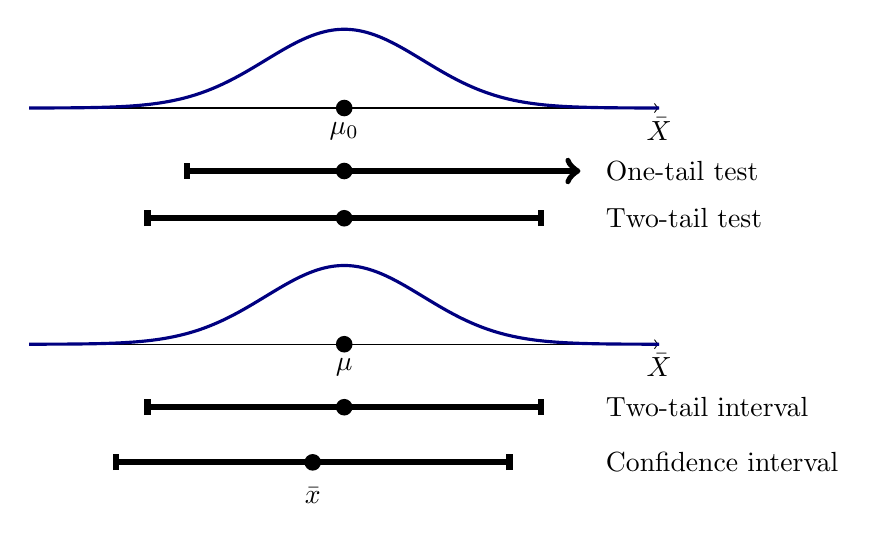
\begin{tikzpicture}
			% First normal distribution
			\draw[->] (-4,0) -- (4,0) node[anchor=north] {$\bar{X}$};
			\draw[line width=.4mm, color=NavyBlue, domain=-4:4, smooth, samples=100] 
			plot (\x, {exp(-0.5*\x*\x)});
			\draw[thick] (0,0.05) -- (0,-0.05) node[anchor=north] {$\mu_0$};
			\fill (0,0) circle (3pt);
			
			% One-sided 95% region
			\draw[->, line width=.8mm] (-2, -0.8) -- (3, -0.8);
			\draw[line width=.8mm] (-2, -0.9) -- (-2, -0.7);
			\fill (0, -0.8) circle (3pt);
			\node[anchor=west] at (3.2, -0.8) {One-tail test};
			
			% Two-sided 95% region
			\draw[line width=.8mm] (-2.5, -1.4) -- (2.5, -1.4);
			\draw[line width=.8mm] (-2.5, -1.5) -- (-2.5, -1.3);
			\draw[line width=.8mm] (2.5, -1.5) -- (2.5, -1.3);
			\fill (0, -1.4) circle (3pt);
			\node[anchor=west] at (3.2, -1.4) {Two-tail test};
			
			% Second normal distribution (below)
			\begin{scope}[shift={(0,-3)}]
				\draw[->] (-4,0) -- (4,0) node[anchor=north] {$\bar{X}$};
				\draw[line width=.4mm, color=NavyBlue, domain=-4:4, smooth, samples=100] 
				plot (\x, {exp(-0.5*\x*\x)});
				\draw[thick] (0,0.05) -- (0,-0.05) node[anchor=north] {$\mu$};
				\fill (0,0) circle (3pt);
				
				% Two-sided CI around mu
				\draw[line width=.8mm] (-2.5, -0.8) -- (2.5, -0.8);
				\draw[line width=.8mm] (-2.5, -0.9) -- (-2.5, -0.7);
				\draw[line width=.8mm] (2.5, -0.9) -- (2.5, -0.7);
				\fill (0, -0.8) circle (3pt);
				\node[anchor=west] at (3.2, -0.8) {Two-tail interval};
				
				% One realised CI shifted left
				\draw[line width=.8mm] (-2.9, -1.5) -- (2.1, -1.5);
				\draw[line width=.8mm] (-2.9, -1.6) -- (-2.9, -1.4);
				\draw[line width=.8mm] (2.1, -1.6) -- (2.1, -1.4);
				\fill (-0.4, -1.5) circle (3pt);
				\node[anchor=north] at (-0.4, -1.7) {$\bar{x}$};
				\node[anchor=west] at (3.2, -1.5) {Confidence interval};
			\end{scope}
		\end{tikzpicture}
	\end{center}
	\begin{itemize}
		\item $\mu_0$ is a {\it hypothesised} mean: ``does my sample mean lie in this interval?''
		\item $\mu$ is the true mean, but is {\it unknown}.
		\item Assume variance $\sigma^2<\infty$ is known and sample size is large.
	\end{itemize}
\end{frame}

\begin{frame}
	\frametitle{Confidence intervals}
	By construction (for the sampling distribution of $\bar X_n$),
	\[
	P\left(\mu - z_{\alpha/2}\frac{\sigma}{\sqrt n}
	<\bar X_n<
	\mu + z_{\alpha/2}\frac{\sigma}{\sqrt n}\right)=1-\alpha.
	\]
	For an observed sample mean $\bar x$, we define the $100(1-\alpha)\%$ confidence interval
	\[
	CI_{\alpha}(\bar x)=\left(\bar x-z_{\alpha/2}\frac{\sigma}{\sqrt n},
	\bar x+z_{\alpha/2}\frac{\sigma}{\sqrt n}\right).
	\]
	{\bf Warning: do not make probabilistic statements about $\mu$}, e.g.
	\begin{quote}
		``There is a $95\%$ chance that $\mu$ lies in this particular interval.''
	\end{quote}
	Interpretation (frequentist): if we repeat the sampling process many times and build such intervals, then a proportion $1-\alpha$ of them will contain $\mu$.
\end{frame}

\begin{frame}
	\frametitle{Example 8C}
	A company is evaluating the effectiveness of two different advertising campaigns, Campaign A and Campaign B, in increasing product sales. They collect sales data from two large, independent regions where each campaign was run. The results are:
	\begin{itemize}
		\item Campaign A: sample size $n_1 = 200$, sample mean $\bar{x}_1 = 520$, population standard deviation $\sigma_1 = 50$.
		\item Campaign B: sample size $n_2 = 250$, sample mean $\bar{x}_2 = 500$, population standard deviation $\sigma_2 = 60$.
	\end{itemize}
	\begin{enumerate}[(a)]
		\item Construct a 95\% confidence interval for the mean sales of Campaign A.
		\item Construct a 95\% confidence interval for the mean sales of Campaign B.
		\item Based on your confidence intervals from (a) and (b), determine whether there is evidence of a significant difference in mean sales between the two campaigns. Explain your reasoning.
	\end{enumerate}
\end{frame}

\begin{frame}
	\frametitle{Example 8C (answer)}
	(a) The formula for a CI when the population standard deviation is known is
	\[
	CI_{\alpha} = \bar{x} \pm z_{\alpha/2} \times \frac{\sigma}{\sqrt{n}}.
	\]
	For a 95\% confidence level, $z_{\alpha/2} = z_{0.975} \approx 1.96$.
	\[
	CI_A = 520 \pm 1.96 \times \frac{50}{\sqrt{200}}
	= 520 \pm 1.96 \times 3.54
	= 520 \pm 6.94
	= (513.06, 526.94).
	\]
	(b) Similarly,
	\[
	CI_B = 500 \pm 1.96 \times \frac{60}{\sqrt{250}}
	= 500 \pm 1.96 \times 3.80
	= 500 \pm 7.45
	= (492.55, 507.45).
	\]
	(c) The CI for Campaign A is $(513.06, 526.94)$ and for Campaign B is $(492.55, 507.45)$. These intervals do not overlap, so at the 95\% level there is statistical evidence of a difference in mean sales between the two campaigns.
\end{frame}

\begin{frame}
	\frametitle{Confidence intervals}
	Warning: so far, we have only considered cases where the $z$-test is appropriate. \par
	In practice, the population variance is usually unknown, so we must estimate it from the sample — these are called {\it nuisance parameters}. \par
	When the variance is unknown, the $t$-distribution is often required to account for the additional uncertainty in estimation. \par
	In the MATH163 exam, you will be told which test to use,
	\begin{itemize}
		\item but you will have to justify the choice of test.
	\end{itemize}
\end{frame}

\begin{frame}
	\frametitle{Link between $z$-tests and confidence intervals}
	Consider testing
	\[
	H_0:\mu=\mu_0 \quad\text{vs.}\quad H_1:\mu\neq\mu_0
	\]
	at significance level $\alpha$, assuming $\sigma^2$ known and $n$ large (so a $z$-test is appropriate).
	\begin{itemize}
		\item The $100(1-\alpha)\%$ confidence interval for $\mu$ is
		\[
		CI_{\alpha}(\bar x)=\left(\bar x-z_{\alpha/2}\frac{\sigma}{\sqrt n},
		\bar x+z_{\alpha/2}\frac{\sigma}{\sqrt n}\right).
		\]
		\item The $z$-test rejects $H_0$ if
		\[
		|z| = \left|\frac{\bar x-\mu_0}{\sigma/\sqrt n}\right| > z_{1-\alpha/2}.
		\]
	\end{itemize}
	{\bf Key fact:}
	\begin{itemize}
		\item Rejecting $H_0$ at level $\alpha$ is {\it equivalent} to $\mu_0$ lying {\bf outside} the $100(1-\alpha)\%$ confidence interval.
		\item If $\mu_0$ lies {\bf inside} the confidence interval, we fail to reject $H_0$ at level $\alpha$.
	\end{itemize}
	{\small\color{NavyBlue}
		Hypothesis tests and confidence intervals are two ways of presenting the same information. \par 
		If you quote a 95\% CI and then report ``the null value lies outside the CI", you have implicitly done a 5\% level test.
	}
\end{frame}

\begin{frame}
	\frametitle{Boxplots vs confidence intervals}
	
	\small
	Three different studies all reporting on the \textbf{same quantity} (a mean). \par
	The boxplots below summarise the sample data. The sample means and 95\% CIs are show in blue. 
	
	\vspace{4pt}
	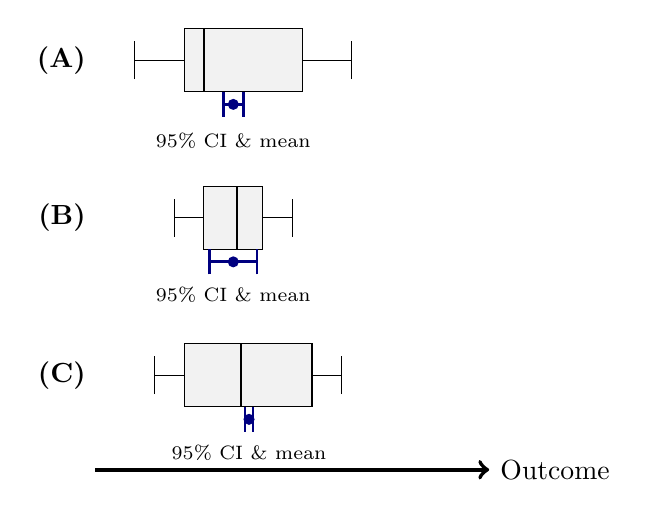
\begin{tikzpicture}[x=0.25cm,y=0.8cm]
		
		% --- Common x-axis ---
		\draw[->,line width=1.5pt] (0,-3) -- (20,-3) node[right] {Outcome};
		
		% ======================================================
		% (A) Skewed data, relatively narrow CI
		% ======================================================
		\node[left] at (0,3.5) {\textbf{(A)}};
		
		% whiskers: clearly right-skewed
		\draw (2,3.5) -- (4.5,3.5);      % left whisker
		\draw (10.5,3.5) -- (13,3.5);    % right whisker
		\draw (2,3.2) -- (2,3.8);
		\draw (13,3.2) -- (13,3.8);
		
		% box (strong right skew: long upper side)
		\draw[fill=gray!10] (4.5,3) rectangle (10.5,4);
		
		% median: noticeably left of centre
		\draw[thick] (5.5,3) -- (5.5,4);
		
		% CI for mean (symmetric, reasonably tight)
		\draw[line width=1pt,color=NavyBlue] (6.5,2.8) -- (7.5,2.8);
		\draw[line width=1pt,color=NavyBlue] (6.5,2.6) -- (6.5,3);
		\draw[line width=1pt,color=NavyBlue] (7.5,2.6) -- (7.5,3);
		
		% sample mean in middle of CI
		\fill[NavyBlue] (7,2.8) circle (2pt);
		
		% label
		\node[below] at (7,2.5) {\scriptsize 95\% CI \& mean};
		
		% ======================================================
		% (B) Moderate spread, wide CI (e.g. smaller n)
		% ======================================================
		\node[left] at (0,1) {\textbf{(B)}};
		
		% whiskers: moderate range
		% range length = 6  (4 to 10)
		\draw (4,1.0) -- (5.5,1.0);      % left whisker
		\draw (8.5,1.0) -- (10,1.0);     % right whisker
		\draw (4,0.7) -- (4,1.3);
		\draw (10,0.7) -- (10,1.3);
		
		% box: roughly symmetric, moderate spread
		\draw[fill=gray!10] (5.5,0.5) rectangle (8.5,1.5);
		
		% median: slightly off-centre
		\draw[thick] (7.2,0.5) -- (7.2,1.5);
		
		% CI for mean: noticeably wide compared to data
		\draw[line width=1pt,color=NavyBlue] (5.8,0.3) -- (8.2,0.3);
		\draw[line width=1pt,color=NavyBlue] (5.8,0.1) -- (5.8,0.5);
		\draw[line width=1pt,color=NavyBlue] (8.2,0.1) -- (8.2,0.5);
		
		% sample mean in middle of CI
		\fill[NavyBlue] (7,0.3) circle (2pt);
		
		\node[below] at (7,0.05) {\scriptsize 95\% CI \& mean};
		
		% ======================================================
		% (C) Wide spread, tight CI (large n)
		% ======================================================
		\node[left] at (0,-1.5) {\textbf{(C)}};
		
		% whiskers: wide range (about 1.5 x B)
		% B range = 10 - 4 = 6
		% C range ≈ 9.5: 3 to 12.5
		\draw (3,-1.5) -- (4.5,-1.5);      % left whisker
		\draw (11,-1.5) -- (12.5,-1.5);    % right whisker
		\draw (3,-1.8) -- (3,-1.2);
		\draw (12.5,-1.8) -- (12.5,-1.2);
		
		% box: wide (larger spread of data)
		\draw[fill=gray!10] (4.5,-2.0) rectangle (11,-1.0);
		
		% median: slightly off-centre
		\draw[thick] (7.4,-2) -- (7.4,-1);
		
		% CI for mean: very tight relative to spread
		\draw[line width=1pt,color=NavyBlue] (7.6,-2.2) -- (8,-2.2);
		\draw[line width=1pt,color=NavyBlue] (7.6,-2.4) -- (7.6,-2.0);
		\draw[line width=1pt,color=NavyBlue] (8,-2.4) -- (8,-2.0);
		
		% sample mean in middle of CI
		\fill[NavyBlue] (7.8,-2.2) circle (2pt);
		
		\node[below] at (7.8,-2.45) {\scriptsize 95\% CI \& mean};
		
	\end{tikzpicture}
	
	%(A) Strongly skewed data, but CI symmetric around the mean. \\
	%(B) CI is large compared to the data spread (imprecise mean). \\
	%(C) CI is small compared to the data spread (precise mean; likely large $n$). \\
	
\end{frame}

\begin{frame}
	\frametitle{Boxplots vs confidence intervals: what do they show?}
	
	\small
	Using plots (A), (B), and (C) from the previous slide:
	
	\begin{enumerate}[(1)]
		\item Look only at the \textbf{boxplots} (ignore the blue dots and CIs): 
		%\begin{itemize}
		%\item 
		For each of A, B, C, what features can you see?
		(centre, spread, skewness, possible outliers)
		%\item Are these features describing:
		%      \textbf{(i)} the sample you have, or
		%      \textbf{(ii)} uncertainty about the true mean $\mu$?
		%\end{itemize}
		
		\item Now look only at the \textbf{confidence intervals and blue dots}:
		\begin{itemize}
			%\item In all three cases, the blue dot is in the centre of the interval.
			%      What quantity does the blue dot represent?
			\item What does the \emph{width} of each interval represent?
			%(Think: how sure are we about the value of $\mu$?)
			\item Do the CIs tell you anything about skewness or the overall shape
			of the data?
		\end{itemize}
		
		\item Compare (B) and (C): what does this suggest about the sample sizes in (B) vs (C)?
		
		\item When can 2 samples have the same box plot but different CIs around the mean
		
		\item When can 2 samples have the same CI around the mean but distinct box plots?
		
		\item \textbf{Key conclusion – complete these sentences:}
		\begin{itemize}
			\item A boxplot is a summary of the \underline{\hspace{2cm}}.
			\item A confidence interval is a summary of our \underline{\hspace{3cm}}
			about the \underline{\hspace{2cm}}.
		\end{itemize}
	\end{enumerate}
	
	%\vspace{4pt}
	%{\small\color{NavyBlue}
		%  Hint: think ``sample distribution'' vs ``uncertainty about the population mean''.
		%}
	
\end{frame}


% ============================================================
% Week 9
% ============================================================

\section{Week 9: statistical testing II}

\begin{frame}
	\frametitle{Comparing distributions}
	$z$-tests: we compare a sample mean against a population mean \par
	More generally, we compare an estimator with a parameter \par
	What if instead we compare \emph{distributions}? \par
	Consider discrete data (categorical or numeric) \par
	Note: this approach can be used with continuous data, but we need to ``bin" it first \par
	% - you will not be asked to do this in MATH163 \par 
	{\bf Question: was my sample drawn from the distribution I think it was drawn from?} \par
	{\bf Goodness of fit test:} does my hypothesised distribution ``fit" the sample?
\end{frame}

\begin{frame}
	\frametitle{Example 9A}
	We roll a dice 60 times. Outcomes are tracked in the table below:
	\begin{center}
		\begin{tabular}{r|cccccc}
			Outcome $i$ & 1 & 2 & 3 & 4 & 5 & 6 \\ \hline
			Frequency & 8 & 10 & 12 & 9 & 0 & 21 \\
		\end{tabular}
	\end{center}
	Is this a fair dice? \par
	If it were then the {\bf expected frequencies} would be:
	\begin{center}
		\begin{tabular}{r|cccccc}
			Outcome $i$ & 1 & 2 & 3 & 4 & 5 & 6 \\ \hline
			Frequency & 10 & 10 & 10 & 10 & 10 & 10 \\
		\end{tabular}
	\end{center}
	$H_0$: the dice is fair \par
	$H_1$: the dice is not fair \par
	Can we compute a single test statistic measuring deviation from expectation?
\end{frame}

\begin{frame}
	\frametitle{Example 9A (setup)}
	In MATH163 we will only consider finite discrete distributions \par
	Let $Y$ be a finite discrete random variable. \par
	Label the outcomes $1,2,\dots,k$ and define $p_i=P(Y=i),\ i=1,2,\dots,k$ so that $\sum_{i=1}^kp_i=1$ \par
	Let $Y_1,Y_2,\dots,Y_n$ be i.i.d.\ random variables following the distribution of $Y$ \par
	Let $c_i$ be the frequency of each outcome measured in our data \par
	From the WLLN, we expect:
	$$\frac {c_i}n\approx p_i\quad\forall i$$
	i.e. $c_i-np_i\approx 0$ \par
	{\bf\underline{Definition}} \par
	The ``chi-squared statistic" is defined as:
	$$\mathcal{X}^2:=\sum_{i=1}^k\frac{(c_i-np_i)^2}{np_i}
	=n\sum_{i=1}^k\frac{\left(\frac{c_i}n-p_i\right)^2}{p_i}$$
\end{frame}

\begin{frame}
	\frametitle{General case}
	{\bf\underline{Theorem}} \par
	If our data $c_i$ are sampled from i.i.d.\ random variables $Y_1,Y_2,\dots,Y_n$ with probabilities $p_i$ then:
	\[
	\mathcal{X}^2\xrightarrow{d}\chi^2_{k-1}\quad\text{as}\quad n\rightarrow\infty
	\]
	where
	\[
	\chi^2_{k-1}\stackrel{d}{=}\sum_{i=1}^{k-1}Z_i^2,\quad Z_i\sim N(0,1)\ \forall i
	\]
\end{frame}

\begin{frame}
	\frametitle{General case: intuition}
	Aside: for each $i$, we could define the indicator variable $\mathbf 1_{Y_j=i}$ and apply the CLT to the binomial distribution $Bin(n,p_i)$:
	$$\frac{(c_i-np_i)^2}{np_i(1-p_i)}\approx Z_i^2$$
	{\bf - but this ignores the fact that the frequencies for different outcomes depend on each other!} \par
	The $\mathcal{X}^2$ statistic retains information about the {\bf whole distribution of data}: \par
	$$\mathcal{X}^2:=\sum_{i=1}^k\frac{(c_i-np_i)^2}{np_i}$$
	The denominator here is {\bf not} a variance term: \par
	\begin{itemize}
		\item $\mathcal{X}^2$ comes from a Poisson approximation to a multinomial distribution (not covered in MATH163)
		\item Variance measures distance from the mean of a random variable \par
		\item $\mathcal{X}^2$ measures distance between observed and expected counts under $H_0$
	\end{itemize}
\end{frame}

\begin{frame}
	\frametitle{$\chi^2$ test}
	We perform a $\chi^2$ test by first choosing a significance level $\alpha\in(0,1)$ \par
	Next we compute $\mathcal{X}^2$, and let $X\sim\chi^2_{k-1}$ \par
	Option 1: \par
	Compute $x=\chi^2_{k-1,\alpha}$ such that $P(X\geq x)=\alpha$ \par
	and reject $H_0$ if $\mathcal{X}^2>x$ \par
	Option 2: \par
	Compute
	\[
	p=P(X\geq\mathcal{X}^2)
	\]
	and reject $H_0$ if $p<\alpha$ \par
	Note: smaller $p$ corresponds to a larger sum of scaled squared deviations from expected outcomes under $H_0$ \par
	\begin{itemize}
		\item The {\bf rejection region} is $[\chi^2_{k-1,\alpha},\infty)$
		\item The {\bf $p$-value} is $P(X\geq\mathcal{X}^2)$
	\end{itemize}
\end{frame}

\begin{frame}
	\frametitle{$\chi^2$ distribution}
	\begin{columns}
		\column{0.5\textwidth}
		\centering
		\fbox{\includegraphics[width=\textwidth]{chi2.png}}\\[3pt]
		$\chi^2$ distribution PDF
		\column{0.5\textwidth}
		\centering
		\fbox{\includegraphics[width=\textwidth]{chi2rejection.png}}\\[3pt]
		Rejection region at 5\% significance level ($\chi^2_5$)
	\end{columns}
\end{frame}

\begin{frame}
	\frametitle{Example 9A (answer)}
	Recall the potentially biased dice:
	\begin{center}
		\begin{tabular}{r|cccccc}
			Outcome $i$ & 1 & 2 & 3 & 4 & 5 & 6 \\ \hline
			Frequency $O_i$ & 8 & 10 & 12 & 9 & 0 & 21 \\ 
			Expectation $E_i$ & 10 & 10 & 10 & 10 & 10 & 10 \\ 
		\end{tabular}
	\end{center}
	\[
	\mathcal{X}^2 = \sum_{i=1}^k \frac{(O_i - E_i)^2}{E_i}
	\]
	Substituting values:
	\begin{align*}
		\mathcal{X}^2 &= \frac{(8 - 10)^2}{10} + \frac{(10 - 10)^2}{10} + \frac{(12 - 10)^2}{10} + \frac{(9 - 10)^2}{10} + \frac{(0-10)^2}{10} + \frac{(21 - 10)^2}{10} \\
		&= \frac{4}{10} + 0 + \frac{4}{10} + \frac{1}{10} + \frac{100}{10} + \frac{121}{10} \\
		&= 0.4 + 0 + 0.4 + 0.1 + 10 + 12.1 \\
		&= 23
	\end{align*}
	Here $k=6$ outcomes, so $df=k-1=5$. \par
	If $X\sim\chi^2_{5}$ then $P(X>14)\approx 0.01561<0.05$ and so we reject $H_0$ at the 5\% significance level.
\end{frame}

\begin{frame}
	\frametitle{Warning}
	We need large enough sample sizes for this approach to be valid: \par
	$$np_i\geq 5\quad\forall i\quad\text{(equivalently: all expected frequencies }E_i\geq 5)$$
	Otherwise we have $2$ options:
	\begin{itemize}
		\item Add more data
		\item Combine outcomes (i.e.\ merge categories to increase expected frequencies)
	\end{itemize}
\end{frame}

\begin{frame}
	\frametitle{Degrees of freedom}
	{\bf\underline{Question}} \par
	With $k$ outcomes, why is $\mathcal{X}^2$ distributed like a sum of $k-1$ squares of standard normal variables? \par
	Intuition:
	\begin{itemize}
		\item The $k$ observed frequencies are constrained by $\sum_i c_i=n$ (one linear constraint)
		\item So only $k-1$ of them can vary freely
		\item This gives $k-1$ effective degrees of freedom
	\end{itemize}
	Second application: testing for independence \par
	{\bf Test of independence: are these $2$ categorical variables independent within a population?}
\end{frame}

\begin{frame}
	\frametitle{Example 9B}
	We want to test if there is an association between gender (male/female) and preference for a new product (like/dislike):
	\begin{center}
		\begin{tabular}{ c | c  c | c }
			& Like & Dislike & Total \\ \hline
			Female & 50 & 20 & 70 \\ 
			Male & 40 & 30 & 70 \\ \hline
			Total & 90 & 50 & 140
		\end{tabular} 
	\end{center}%\par 
	Note the following:
	\begin{itemize}
		\item The data are partitioned by $2$ different variables (rows and columns)
		\item $H_0:$ Gender and preference are independent, e.g. $P(L\vert F)=P(L\vert M)=P(L)$
		\item We {\it could} have more rows (groups) or columns (categories)
	\end{itemize}
	{\bf\underline{Questions}} \par
	\begin{itemize}
		\item What is $H_1$?
		\item How many degrees of freedom do we have?
		\item Do we have enough evidence to reject $H_0$ at the 5\% significance level?
	\end{itemize}
\end{frame}

\begin{frame}
	\frametitle{Example 9B (answer)}
	{\bf\underline{Answers}} \par
	$H_1$: Gender and preference are not independent \par
	\begin{columns}
		\column{0.5\textwidth}
		\centering
		\begin{tabular}{ c | c  c | c }
			& Like & Dislike & Total \\ \hline
			Female & 50$^{(1)}$ & 20$^{(2)}$ & 70 \\ 
			Male & 40$^{(3)}$ & 30$^{(4)}$ & 70 \\ \hline
			Total & 90 & 50 & 140
		\end{tabular}\\[3pt]
		Original table
		\column{0.5\textwidth}
		\centering
		\begin{tabular}{ c | c  c | c }
			& Like & Dislike & Total \\ \hline
			Female & 45$^{(1)}$ & 25$^{(2)}$ & 70 \\ 
			Male & 45$^{(3)}$ & 25$^{(4)}$ & 70 \\ \hline
			Total & 90 & 50 & 140
		\end{tabular}\\[3pt]
		Expected values under $H_0$
	\end{columns}
	Our data gives us the row and column sums, so in a $2\times 2$ table we have
	\[
	df=(2-1)(2-1)=1.
	\]
	Note that $n$ does not feature explicitly in the $\mathcal{X}^2$ formula, but it does appear in the expected counts $E_{ij}$.
\end{frame}

\begin{frame}
	\frametitle{Example 9B (answer)}
	Compute the $\mathcal{X}^2$ statistic:
	\begin{eqnarray*}
		\mathcal{X}^2&=&\frac{(50-45)^2}{45}+\frac{(20-25)^2}{25}+\frac{(40-45)^2}{45}+\frac{(30-25)^2}{25}\\
		&=&\frac{25}{45}+\frac{25}{25}+\frac{25}{45}+\frac{25}{25}\\
		&=&3.111\ (\text{approximately})
	\end{eqnarray*}
	With $df=1$, this gives $p\approx 0.146$, so we do not reject $H_0$ at the 5\% significance level. \par
	There is not enough evidence (at 5\%) to conclude that gender and preference are associated.
\end{frame}

\begin{frame}
	\frametitle{$2\times 2$ tables: the quick way}
	Given the following \(2 \times 2\) contingency table:
	\[
	\begin{array}{c|cc|c}
		& \text{Category 1} & \text{Category 2} & \text{Row Total} \\ \hline
		\text{Group 1} & a & b & a + b \\
		\text{Group 2} & c & d & c + d \\ \hline
		\text{Column Total} & a + c & b + d & N
	\end{array}
	\]
	Under the null hypothesis of independence, the expected values for each cell are:
	\[
	E_{ij} = \frac{(\text{row total}) \times (\text{column total})}{N}.
	\]
	This leads to the shortcut formula:
	\[
	\chi^2 = \frac{N(ad - bc)^2}{(a + b)(c + d)(a + c)(b + d)}.
	\]
	This still has $df=1$.
\end{frame}

\begin{frame}
	\frametitle{Degrees of freedom (general)}
	When we have an $m\times n$ table of frequencies, how many degrees of freedom do we have?
	\begin{center}
		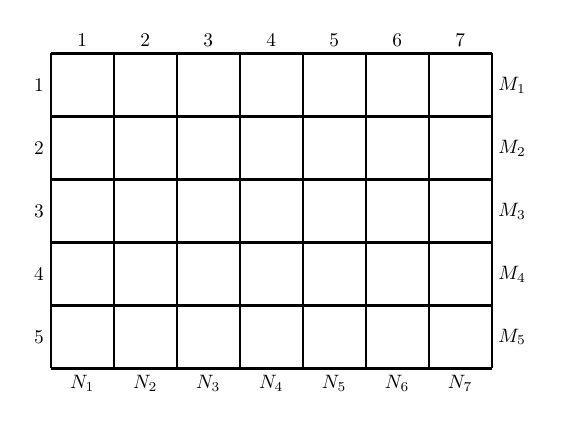
\begin{tikzpicture}[scale=0.8]
			\def\nrow{5}
			\def\ncol{7}
			% grid
			\foreach \x in {0,...,\ncol} {
				\draw[thick] (\x,0) -- (\x,\nrow);
			}
			\foreach \y in {0,...,\nrow} {
				\draw[thick] (0,\y) -- (\ncol,\y);
			}
			% row sums
			\foreach \y in {1,...,\nrow} {
				\node[right,scale=0.7] at (\ncol,\nrow-\y+0.5) {$M_{\y}$};
			}
			% column sums
			\foreach \x in {1,...,\ncol} {
				\node[below,scale=0.7] at (\x-0.5,0) {$N_{\x}$};
			}
			% row numbers
			\foreach \y in {1,...,\nrow} {
				\node[left,scale=0.7] at (0,\nrow-\y+0.5) {\y};
			}
			% column numbers
			\foreach \x in {1,...,\ncol} {
				\node[above,scale=0.7] at (\x-0.5,\nrow) {\x};
			}
		\end{tikzpicture}
	\end{center}
\end{frame}

\begin{frame}
	\frametitle{Degrees of freedom (general)}
	When we have an $m\times n$ table of frequencies, how many degrees of freedom do we have?
	\begin{center}
		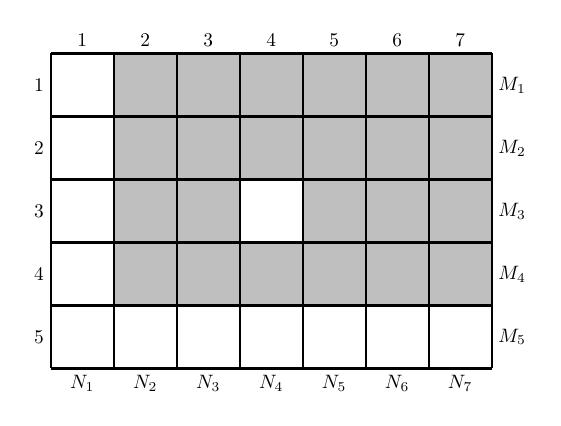
\begin{tikzpicture}[scale=0.8]
			\def\nrow{5}
			\def\ncol{7}
			% shade (nrow-1)x(ncol-1) block
			\foreach \x in {1,...,6} {
				\foreach \y in {1,...,4} {
					\fill[gray!50] (\x,\y) rectangle ++(1,1);
				}
			}
			% highlight one cell
			\fill[white] (3,2) rectangle ++(1,1);
			% grid
			\foreach \x in {0,...,\ncol} {
				\draw[thick] (\x,0) -- (\x,\nrow);
			}
			\foreach \y in {0,...,\nrow} {
				\draw[thick] (0,\y) -- (\ncol,\y);
			}
			% row sums
			\foreach \y in {1,...,\nrow} {
				\node[right,scale=0.7] at (\ncol,\nrow-\y+0.5) {$M_{\y}$};
			}
			% column sums
			\foreach \x in {1,...,\ncol} {
				\node[below,scale=0.7] at (\x-0.5,0) {$N_{\x}$};
			}
			% row numbers
			\foreach \y in {1,...,\nrow} {
				\node[left,scale=0.7] at (0,\nrow-\y+0.5) {\y};
			}
			% column numbers
			\foreach \x in {1,...,\ncol} {
				\node[above,scale=0.7] at (\x-0.5,\nrow) {\x};
			}
		\end{tikzpicture}
	\end{center}
	Our data give the row and column totals, so we have $(m-1)\times(n-1)$ degrees of freedom. \par
	This only applies when $m,n>1$ (otherwise there is no true ``table" structure).
\end{frame}

\begin{frame}
	\frametitle{Example 9C}
	A study is conducted to examine the growth of bulbs planted in different locations. A total of $370$ gardeners each plant $4$ bulbs and record how many successfully sprout after 3 weeks. The observed results are:
	\begin{center}
		\begin{tabular}{r|ccccc}
			Number of bulbs sprouted & 0 & 1 & 2 & 3 & 4 \\ \hline
			Frequency & 12 & 54 & 107 & 130 & 67 \\
		\end{tabular}
	\end{center}
	It is assumed that these results follow a binomial distribution $Bin(4,p)$ for some probability 
	$p$, which is estimated using the overall proportion of bulbs that sprouted. \par
	Perform a $\chi^2$ goodness of fit test to assess whether the binomial model provides a suitable fit for the data at the 5\% significance level. \par
	Note: this is a goodness of fit test.
\end{frame}

\begin{frame}
	\frametitle{Example 9C (answer)}
	%{\bf\underline{Answer}} \par
	$H_0$: $X\sim Bin(4,p)$, \quad $H_1$: $X\nsim Bin(4,p)$ \par
	Note: we have not made a hypothesis about $p$ - we need to estimate it from the data. \par
	Since each gardener plants $4$ bulbs, the total number of planted bulbs is $370 \times 4 = 1480$ \par
	The total number of successful sprouts is \\
	$(0 \times 12) + (1 \times 54) + (2 \times 107) + (3 \times 130) + (4 \times 67) = 926$ \par
	The estimated probability of sprouting is therefore
	\[
	\hat p=\frac{926}{1480} \approx 0.626.
	\]
	The expected frequencies are given by $E_k = 370 \times P(X = k)$:
	\begin{center}
		\begin{tabular}{r|ccccc}
			Number of bulbs sprouted & 0 & 1 & 2 & 3 & 4 \\ \hline
			Frequency $O_i$ & 12 & 54 & 107 & 130 & 67 \\ 
			Expected frequency $E_i$ & 7.24 & 48.47 & 121.69 & 135.79 & 56.82 \\ 
		\end{tabular}
	\end{center}
	This gives:
	\begin{eqnarray*}
		\mathcal{X}^2 &=& \frac{(12 - 7.24)^2}{7.24} + \frac{(54 - 48.47)^2}{48.47} + \frac{(107 - 121.69)^2}{121.69} \\
		&&\quad + \frac{(130 - 135.79)^2}{135.79} + \frac{(67 - 56.82)^2}{56.82}\\
		&\approx& 7.605.
	\end{eqnarray*}
\end{frame}

\begin{frame}
	\frametitle{Degrees of freedom (with estimated parameters)}
	Recall that using the sample mean to compute sample variance reduces the effective sample size by $1$ \par
	- this is the loss of a degree of freedom. \par
	In general, if we have $n$ categories, then:
	\[
	df = n - 1 - \text{(number of estimated parameters)}.
	\]
	If we have an $m\times n$ table, then:
	\[
	df = (m-1)(n-1) - \text{(number of estimated parameters)}.
	\]
\end{frame}

\begin{frame}
	\frametitle{Example 9C: (answer)}
	Here $n=5$ categories and we estimated one parameter $p$, so:
	\[
	df = n - 1 - 1 = 5-1-1=3.
	\]
	The critical value for \( \alpha = 0.05 \) and \( df = 3 \) is approximately $7.815$. \par
	Since \( \mathcal{X}^2 = 7.605 < 7.815 \), we fail to reject \( H_0 \) at the 5\% significance level. \par
	This suggests that the binomial assumption is reasonable. \par
	The critical value for \( \alpha = 0.1 \) and \( df = 3 \) is approximately $6.251$, \par
	so we would reject $H_0$ at the 10\% significance level.
\end{frame}

\begin{frame}
	\frametitle{$\chi^2$ test: summary}
	\begin{enumerate}
		\item State $H_0$ and $H_1$.
		\item Complete the following table:
		\begin{center}
			\begin{tabular}{ r || c | c | c | c | c | c |}
				Value $i$ & 0 & 1 & 2 & 3 & 4 & \dots\\ \hline
				$O_i$ &  &  &  &  &  &  \\ \hline
				$E_i$ &  &  &  &  &  &  \\ \hline
				$O_i-E_i$ &  &  &  &  &  &  \\ \hline
				$(O_i-E_i)^2$ &  &  &  &  &  &  \\ \hline
				$(O_i-E_i)^2/E_i$ &  &  &  &  &  &  \\ \hline
			\end{tabular}
		\end{center}
		\item Compute $\mathcal{X}^2=\sum_{i=1}^k(O_i-E_i)^2/E_i$.
		\item Compute the degrees of freedom: \\
		$1$ variable: $df = n - 1 -$ (number of estimated parameters) \\
		$2$ variables: $df = (m-1)(n-1) -$ (number of estimated parameters).
		\item Compute the value $x$ such that $P(X\geq x)=\alpha$, where $X\sim\chi^2_{df}$, \\
		or compute the $p$-value $P(X\geq \mathcal{X}^2)$.
		\item Decide whether to reject $H_0$ at significance level $100\alpha\%$.
	\end{enumerate}
\end{frame}

\begin{frame}
	\frametitle{Example 9D: test of homogeneity}
	{\bf Test of homogeneity:} is the distribution of a categorical variable the same across different groups? \par 
	A hospital network is evaluating the effectiveness of a new treatment across three hospitals. Each hospital administers the same treatment, and doctors record whether the treatment was successful or unsuccessful. The observed data are:
	\[
	\begin{array}{c|cc|c}
		\text{Hospital} & \text{Success} & \text{Failure} & \text{Total Patients} \\ \hline
		\text{A} & 42 & 18 & 60 \\
		\text{B} & 70 & 30 & 100 \\
		\text{C} & 56 & 34 & 90 \\ \hline
		\text{Total} & 168 & 82 & 250
	\end{array}
	\]
	We assume that the treatment has an underlying probability of success \( p \) that is the same for all hospitals. \par
	Perform a chi-squared test of homogeneity at the 5\% significance level to determine whether the observed success rates differ significantly from the expected rates under the null hypothesis.
	
	\begin{center}
		\fbox{\includegraphics[width=.2\textwidth]{countdown.jpg}}
	\end{center}
\end{frame}

\begin{frame}
	\frametitle{$\chi^2$ tests: three flavours}
	
	\begin{itemize}
		\item \textbf{Goodness-of-fit (GoF):} Are categories in one sample consistent with a known/theoretical distribution?
		\begin{itemize}
			\item \emph{Layout:} one variable, $k$ categories (a single row of counts).
			\item \emph{$H_0$:} sample comes from a specified distribution
			(e.g.\ Poisson, discrete uniform).
			\item \emph{df:} $k - 1 - m$, where $m$ is the number of parameters
			estimated from the data.
			\item \emph{Example (Poisson):}
			\begin{itemize}
				\item $H_0$: counts follow $\text{Pois}(\lambda=8.2)$ (fully specified) $\Rightarrow m=0$, df $=k-1$.
				\item $H_0$: counts follow $\text{Pois}(\lambda)$ with $\lambda$ estimated from the sample $\Rightarrow m=1$, df $=k-2$.
			\end{itemize}
		\end{itemize}
		
		\vspace{4pt}
		\item \textbf{Test of independence (ToI):} Are two categorical variables associated in one population?
		\begin{itemize}
			\item \emph{Layout:} one sample, cross-classified by 2 variables
			in an $r \times c$ contingency table.
			\item \emph{$H_0$:} row and column variables are independent.
			\item \emph{df:} $(r-1)(c-1)$.
		\end{itemize}
		
		\vspace{4pt}
		\item \textbf{Test of homogeneity (ToH):} Are the category distributions the same across several populations?
		\begin{itemize}
			\item \emph{Layout:} several groups, 1 categorical variable,
			arranged in an $r \times c$ table.
			\item \emph{$H_0$:} all groups share the same category distribution.
			\item \emph{df:} $(r-1)(c-1)$.
		\end{itemize}
	\end{itemize}
	
\end{frame}


% ============================================================
% Week 10
% ============================================================

\section{Week 10: statistical testing III}

\begin{frame}
	\frametitle{The $t$-distribution} 
	Recall the CLT: If $X$ has mean $\mu$ and variance $\sigma^2<\infty$ then:
	$$Z:=\frac{\bar X_n-\mu}{\sigma/\sqrt n}\xrightarrow{d} N(0,1)\ \text{as}\ n\rightarrow \infty$$
	{\small\color{NavyBlue} Here the subscript ``$n$" denotes ``samples of size $n$"} \par
	We can use this to test a hypothesized population mean $\mu_0$ \par
	- but what if we do not know $\sigma^2$? \par
	We can approximate $\sigma$ with $S_n$ as follows:
	$$T:=\frac{\bar X_n-\mu}{S_n/\sqrt n}$$
	- but how is this distributed?
\end{frame}

\begin{frame}
	\frametitle{The $t$-distribution} 
	Assume $X_1,\dots,X_n\sim N(\mu,\sigma^2)$ i.i.d. Then:
	\begin{eqnarray*}
		T:&=&\frac{\bar X_n-\mu}{S_n/\sqrt n}
		=\frac{\bar X_n-\mu}{\sigma/\sqrt n}\times\frac{\sigma}{S_n}\\[4pt]
		V:&=&(n-1)\frac{S_n^2}{\sigma^2}\sim\chi^2_{n-1}\\[4pt]
		\Rightarrow T&=&Z\sqrt{\frac{n-1}{V}}\sim t_{n-1}
	\end{eqnarray*}
	{\small\color{NavyBlue} ``$T$ follows a $t$-distribution with $n-1$ degrees of freedom" \par
		- the formula for the PDF of $T$ is horrible and not needed in MATH163 \par
		- we also require that $Z$ and $V$ are independent}
\end{frame}

\begin{frame}
	\frametitle{The $t$-distribution}
	\begin{columns}
		\column{0.5\textwidth}
		\centering
		\fbox{\includegraphics[width=\textwidth]{tdist.png}}\\[3pt]
		$t$-distribution PDF
		\column{0.5\textwidth}
		\centering
		\fbox{\includegraphics[width=\textwidth]{tcdf.png}}\\[3pt]
		$t$-distribution CDF
	\end{columns}
\end{frame}

\begin{frame}
	\frametitle{Single sample $t$-tests} 
	Why $n-1$ degrees of freedom?
	\begin{itemize}
		\item The $(n-1)$ correction in $S^2$ yields an unbiased estimator of $\sigma^2$
		\item This is still an estimate, introducing additional uncertainty into the test statistic
		\item Variability in $S^2$ appears in the denominator of $T$, which gives a heavier-tailed distribution than when $\sigma^2$ is known
	\end{itemize}
\end{frame}

\begin{frame}
	\frametitle{Single sample $t$-tests} 
	Protocol: as with a $z$-test except:
	\begin{itemize}
		\item Use $S^2$ in place of $\sigma^2$ \par
		Warning:
		\begin{eqnarray*}
			S^2&:=&\frac 1{n-1}\sum_{i=1}^n(X_i-\bar X)^2 \\[4pt]
			&=&\frac 1{n-1}\left(\sum_{i=1}^nX_i^2-2\bar X\sum_{i=1}^nX_i+n\bar X^2\right)\\[4pt]
			&=&\frac 1{n-1}\left(\sum_{i=1}^nX_i^2-n\bar X^2\right)\\[4pt]
			&=&\frac 1{n-1}\sum_{i=1}^nX_i^2-\frac n{n-1}\bar X^2
		\end{eqnarray*}
		- this is not quite the ``mean of the square minus the square of the mean"
		\item Probabilities are calculated from the Student's $t$-distribution \par
		{\bf with $n-1$ degrees of freedom}
	\end{itemize}
\end{frame}

\begin{frame}
	\frametitle{Single sample $t$-tests} 
	Protocol: as with a $z$-test except:
	\begin{enumerate}
		\item State $H_0$
		\item State your alternate hypothesis $H_1$
		\item State your significance level ($100\alpha\%$)
		\item Calculate the sample mean $\bar x$, the sample variance $s^2$ and the $t$-statistic:
		$$t:=\frac{\bar x-\mu_0}{s/\sqrt{n}}$$
		\item Find the critical value $t^*_{n-1,\alpha}$ (or $t^*_{n-1,\alpha/2}$ for a two-tail test) corresponding to your significance level \par
		($n-1$ denotes the degrees of freedom in the $t$-distribution)
		\item Decide whether to reject $H_0$
	\end{enumerate}
	{\small\color{NavyBlue} $t$-tables provide critical $t$-values for given significance levels and degrees of freedom}
\end{frame}

\begin{frame}
	\frametitle{Example 10A} 
	How important is it to use the $t$-distribution over the normal distribution? \par
	A researcher is studying the effects of a new tutoring program on student test scores. A small sample of \( n = 8 \) students is selected, and their test score improvements (points gained after tutoring) are recorded in a frequency table:
	
	\[
	\begin{array}{r|cccc}
		\hline
		\text{Improvement points} & 3 & 4 & 5 & 6 \\
		\hline
		\text{Frequency} & 1 & 3 & 2 & 2 \\
		\hline
	\end{array}
	\]
	A national study found that, on average, students improve by \( 4 \) points without tutoring. The researcher wants to determine whether the new tutoring program significantly improves scores.
\end{frame}

\begin{frame}
	\frametitle{Example 10A (answer)}
	We have:
	\begin{eqnarray*}
		H_0:&&\ \mu\leq 4;\qquad H_1:\ \mu>4 \\[4pt]
		\bar{x} &=& \frac 18(3 \times 1 + 4 \times 3 + 5 \times 2 + 6 \times 2)
		= 4.625 \\[4pt]
		s^2 &=& \frac 17(3^2 \times 1 + 4^2 \times 3 + 5^2 \times 2 + 6^2 \times 2)
		-\frac 8{7}\bar x^2
		= 1.125 \\[4pt]
		t &=& \frac{\bar x - \mu_0}{s / \sqrt{n}}
		= \frac{4.625 - 4}{\sqrt{1.125/8}}
		\approx 1.667
	\end{eqnarray*}
	One-tail, 5\% significance level: \par
	\begin{itemize}
		\item $t^*_{7,0.95}=1.895>1.667$ \quad (fail to reject $H_0$)
		\item If we (incorrectly) used a $z$-test with $s$ in place of $\sigma$: \\
		$z^*_{0.95}=1.645<1.667$ \quad (we would reject $H_0$)
	\end{itemize}
	{\small\color{NavyBlue} This shows why the heavier tails of the $t$-distribution matter for small $n$}
\end{frame}

\begin{frame}
	\frametitle{Approximate normality}
	{\bf Warning: working with small sample sizes ($n<30$) requires the population to be approximately normally distributed} \par
	\begin{itemize}
		\item The $t$-distribution accounts for additional variation due to estimating $\sigma^2$ \par
		\item For large $n$, the CLT helps the sampling distribution of $\bar X_n$ to be approximately normal, even if the population is not
		\item For small $n$, we rely much more strongly on the assumption of (approximate) normality in the population
		\item When $n<30$ and the population is clearly non-normal, non-parametric tests should be used
	\end{itemize}
	How can we test for (approximate) normality?
\end{frame}

\begin{frame}
	\frametitle{Checking normality (informally)}
	In practice, before using a $t$- or $z$-test with small $n$, we often:
	\begin{itemize}
		\item Inspect a histogram of the sample
		\item Look at a normal Q–Q plot (sample quantiles vs theoretical normal quantiles)
		\item Check for strong skewness or obvious outliers
	\end{itemize}
	{\small\color{NavyBlue} In MATH163 you will not be required to carry out formal normality tests \par
		- but you should be able to justify assuming (or not assuming) approximate normality based on context}
\end{frame}

\begin{frame}
	\frametitle{Confidence intervals} 
	With unknown population variance, we also use the $t$-distribution to calculate confidence intervals \par
	At confidence level $100(1-\alpha)\%$, we define:
	\begin{eqnarray*}
		CI_{1-\alpha}&=&\left(\bar x-t^*_{n-1,\frac{\alpha}{2}}\frac s{\sqrt n},\ \bar x+t^*_{n-1,\frac{\alpha}{2}}\frac s{\sqrt n}\right) \\[4pt]
		\text{where}\quad s^2&=&\frac 1{n-1}\sum_{i=1}^nx_i^2-\frac n{n-1}\bar x^2
	\end{eqnarray*}
\end{frame}

\begin{frame}
	\frametitle{Example 10B}
	A business analyst is studying the relationship between sales revenue and profit margins. The analyst collects data from 5 small businesses and records their weekly sales revenue (in thousands of dollars). The data is:
	\begin{table}[h]
		\centering
		\begin{tabular}{r|ccccc}
			\hline
			Business & 1 & 2 & 3 & 4 & 5 \\
			\hline
			Sales (\$1000s) & 10 & 12 & 15 & 8 & 14 \\
			\hline
		\end{tabular}
	\end{table}
	Profit is calculated from sales revenue: there is a fixed cost of \$2000 when sales are zero, and each additional \$1000 in sales contributes \$600 to profit after variable costs. \par
	\begin{enumerate}
		\item Compute the sample mean \( \bar{X} \) and standard deviation \( s_X \) of the sales values
		\item Let $Y$ denote profit (in \$1000s). Use a transformation formula to find \( \bar{Y} \) and \( s_Y \)
		\item Construct a 95\% confidence interval for the mean of \( Y \), assuming the data follow a normal distribution
		\item Justify the use of the Student’s $t$-distribution in this context
	\end{enumerate}
\end{frame}

\begin{frame}
	\frametitle{Example 10B (answer)}
	Note: \( Y = 0.6X - 2 \) so $\bar y=0.6\bar x-2$ and \( s_Y = 0.6\, s_X \).
	\begin{eqnarray*}
		\bar{x} &=& \frac{10 + 12 + 15 + 8 + 14}{5} = \frac{59}{5} = 11.8 \\[4pt]
		s_X^2 &=& \frac 14\Big((10 - 11.8)^2 + (12 - 11.8)^2 + (15 - 11.8)^2 + (8 - 11.8)^2 + (14 - 11.8)^2\Big) \\[4pt]
		&=& \frac{32.8}{4} = 8.2,\qquad
		s_X = \sqrt{8.2} = 2.863 \\[4pt]
		\bar{y} &=& 0.6(11.8) - 2 = 5.08 \\[4pt]
		s_Y^2 &=& (0.6)^2 s_X^2 = 0.36(8.2) = 2.952,\qquad
		s_Y = \sqrt{2.952} = 1.718
	\end{eqnarray*}
\end{frame}

\begin{frame}
	\frametitle{Example 10B (answer)}
	Using the Student's $t$-distribution with \( df = n-1 = 4 \) degrees of freedom, the critical value from the $t$-table for 95\% confidence is \( t^* = 2.776 \). \par
	The confidence interval is:
	\begin{eqnarray*}
		CI_{0.95}
		&=&\left(\bar{y}-t^*\times\frac{s_Y}{\sqrt{n}},\ \bar{y}+t^*\times\frac{s_Y}{\sqrt{n}}\right)\\[4pt]
		&\approx&(2.94, 7.22)
	\end{eqnarray*}
	Justification: the population variance of profit is unknown, and the sample size is small (\( n < 30 \)), making the use of the Student’s $t$-distribution appropriate rather than the normal distribution. \\[4pt]
	{\small\color{NavyBlue} Note: in this question, the table had one column per data point – not a frequency table.}
\end{frame}

\begin{frame}
	\frametitle{Example 10C}
	A researcher is studying the effectiveness of a new training program on the success rate of students passing an exam. A random sample of 8 students is selected, and the number of passes per student (out of 2 possible attempts) is recorded in the frequency table below:
	
	\[
	\begin{array}{r|ccc}
		\hline
		\text{Number of Passes} & 0 & 1 & 2 \\
		\hline
		\text{Frequency} & 2 & 3 & 3 \\
		\hline
	\end{array}
	\]
	The researcher hypothesizes that the average number of successful passes is 1.
	\begin{enumerate}
		\item Test the hypothesis at the 5\% significance level
		\item Now, multiply the sample size by 100, maintaining the relative frequencies, and perform the test again. Switch to a $z$-test for the larger sample size. How does the result change?
	\end{enumerate}
\end{frame}

\begin{frame}
	\frametitle{Example 10C (answer)}
	$H_0$: $\mu=1$;\quad $H_1$: $\mu\neq 1$.
	\begin{eqnarray*}
		\bar{x} &=& \frac{2(0) + 3(1) + 3(2)}{2 + 3 + 3} = \frac{9}{8} = 1.125 \\[4pt]
		s^2 &=& \frac{2(0 - 1.125)^2 + 3(1 - 1.125)^2 + 3(2 - 1.125)^2}{8 - 1}
		\approx 0.696 \\[4pt]
		s &\approx& 0.835 \\[4pt]
		t &=& \frac{\bar{X} - \mu_0}{s / \sqrt{n}}
		= \frac{1.125 - 1}{0.835 / \sqrt{8}}
		\approx 0.424 \\[4pt]
		df &=& 8 - 1 = 7 \\[4pt]
		t^*_{7,0.975} &\approx& 2.365>0.424
	\end{eqnarray*}
	- so we fail to reject $H_0$ at the 5\% significance level.
\end{frame}

\begin{frame}
	\frametitle{Example 10C (answer)}
	Multiplying the frequencies by $100$ gives:
	\[
	\begin{array}{r|ccc}
		\hline
		\text{Number of Passes} & 0 & 1 & 2 \\
		\hline
		\text{Frequency} & 200 & 300 & 300 \\
		\hline
	\end{array}
	\]
	$\bar x$ and $s$ remain unchanged, but $n$ is now much larger:
	$$t=\frac{\bar{X} - \mu_0}{s / \sqrt{n}} = \frac{1.125 - 1}{0.835 / \sqrt{800}} \approx 4.24.$$
	For a two-tail 5\% test:
	\begin{itemize}
		\item $z^*_{0.975}=1.96<4.24$
		\item $t^*_{799,0.975}\approx 1.96<4.24$
	\end{itemize}
	So now we reject $H_0$. \par
	{\small\color{NavyBlue} With a large sample, even small deviations from $\mu_0$ can become statistically significant.}
\end{frame}

\begin{frame}
	\frametitle{Further applications}
	The $t$-distribution is not only useful for one-sample tests and CIs, but also has several other applications in statistical inference: \par
	\begin{itemize}
		\item \textbf{One-sample $t$-test}: testing the mean of a single sample against a known value when the population variance is unknown
		\item \textbf{Two-sample $t$-test}: comparing the means of two independent samples to test if they come from populations with the same mean
		\item \textbf{Paired $t$-test}: comparing the means of two related groups (e.g., before and after treatment for the same subjects)
		\item \textbf{Regression analysis}: in simple linear regression, the $t$-distribution is used to test the significance of regression coefficients
	\end{itemize}
	These will not be studied in detail in MATH163.
\end{frame}

\begin{frame}
	\frametitle{$\bigstar$ Statistical testing: summary} 
	You have a sample and a question regarding the sample. \par
	Are you testing a single summary statistic (the mean)?
	\begin{itemize}
		\item {\bf YES:} \par
		Do you have a large sample size ($n\geq 30$) OR an approximately normal population?
		\begin{itemize}
			\item {\bf YES:} 
			Do you know the population variance?
			\begin{itemize}
				\item {\bf YES:} $z$-test
				\item {\bf NO:} $t$-test ($n-1$ degrees of freedom) – approximate $\sigma^2$ with $S^2$
			\end{itemize}
			\item {\bf NO:} Non-parametric test (not in MATH163)
		\end{itemize}
		\item {\bf NO:} $\chi^2$-test \par
		Do you have a $2\times 2$ contingency table?
		\begin{itemize}
			\item {\bf YES:} You may use the ``quick method"
			\item {\bf NO:} Write out the expression for a $\mathcal{X}^2$ statistic
		\end{itemize}
	\end{itemize}
	Across assessments, you will be expected to perform all of these types of tests. \par
	{\small\color{NavyBlue} In the exam you may be told which test to use, but you must be able to justify that choice.}
\end{frame}

\begin{comment}
	1/2 tail test / which type of chi-squared – comes from wording of $H_0$
\end{comment}


\end{document}
